% This LaTeX document needs to be compiled with XeLaTeX.
\documentclass[10pt]{article}
\usepackage[utf8]{inputenc}
\usepackage{graphicx}
\usepackage[export]{adjustbox}
\graphicspath{ {./images/} }
\usepackage{amsmath}
\usepackage{amsfonts}
\usepackage{amssymb}
\usepackage[version=4]{mhchem}
\usepackage{stmaryrd}
\usepackage{hyperref}
\hypersetup{colorlinks=true, linkcolor=blue, filecolor=magenta, urlcolor=cyan,}
\urlstyle{same}
\usepackage[fallback]{xeCJK}
\usepackage{polyglossia}
\usepackage{fontspec}
\setCJKmainfont{Noto Serif CJK SC}

\setmainlanguage{english}
\setmainfont{CMU Serif}

%New command to display footnote whose markers will always be hidden
\let\svthefootnote\thefootnote
\newcommand\blfootnotetext[1]{%
  \let\thefootnote\relax\footnote{#1}%
  \addtocounter{footnote}{-1}%
  \let\thefootnote\svthefootnote%
}

%Overriding the \footnotetext command to hide the marker if its value is `0`
\let\svfootnotetext\footnotetext
\renewcommand\footnotetext[2][?]{%
  \if\relax#1\relax%
    \ifnum\value{footnote}=0\blfootnotetext{#2}\else\svfootnotetext{#2}\fi%
  \else%
    \if?#1\ifnum\value{footnote}=0\blfootnotetext{#2}\else\svfootnotetext{#2}\fi%
    \else\svfootnotetext[#1]{#2}\fi%
  \fi
}

\begin{document}
数学奥林匹克小丛书

\section*{管二版}
\section*{(1)}
\section*{一次函数与二次函数}
李惟峰 编著

目龔华东师范大学出版社\\
EON 等市 全国白健国来出版鱼位

数学奥林匹克小丛书采二版\\

\includegraphics[max width=\textwidth, center]{2024_10_30_1bf34f7aeb61f11d11d3g-002}\\

\includegraphics[max width=\textwidth, center]{2024_10_30_1bf34f7aeb61f11d11d3g-002(1)}\\

\includegraphics[max width=\textwidth, center]{2024_10_30_1bf34f7aeb61f11d11d3g-002(2)}

一次函数与二次函数\\
李惟峰 编著

\section*{图书在版编目(CIP)数据}
数学奥林匹克小丛书. 初中卷. 一次函数与二次函数/李惟峰编著. —2版. 一上海: 华东师范大学出版社, 2011.12

ISBN 978-7-5617-9167-7\\
I. (1) 数..\\
II. (1) 李 …\\
III. (1)代数课一初中一教学参考

资料 IV.(1)G634.603\\
中国版本图书馆 CIP 数据核字(2011)第262645号

数学奥林匹克小丛书(第二版) $\cdot$ 初中卷

\section*{一次函数与二次函数(第二版)}
\begin{center}
\begin{tabular}{|c|c|}
\hline
编 著 & 李惟峰 \\
\hline
总策 划 & 倪 明 \\
\hline
项目编辑 & 孔令志 \\
\hline
审读编辑 & 刘 艺 \\
\hline
装帧设计 & 高 山 \\
\hline
责任发行 & 郑海兰 \\
\hline
出版发行 & 华东师范大学出版社 \\
\hline
社 址 & 上海市中山北路 3663 号 邮编 200062 \\
\hline
网 址 & www. ecnupress. com.cn \\
\hline
电 话 & 021-60821666 行政传真 021-62572105 \\
\hline
客服电话 & 021-62865537 门市(邮购)电话 021-62869887 \\
\hline
地 址 & 上海市中山北路 3663 号华东师范大学校内先锋路口 \\
\hline
网 店 & http://hdsdcbs. tmall.com \\
\hline
\end{tabular}
\end{center}

印 刷 者 常熟高专印刷有限公司\\
开 本 $787 \times 1092$ 16开\\
插 页 1\\
印 张 8.25\\
字 数 144 千字\\
版 次 2012 年 7 月第二版\\
印 次 2012 年 7 月第一次\\
印 数 1—13000\\
书 号 ISBN 978-7-5617-9167-7/G $\cdot$ 5471\\
定 价 16.00 元\\
出 版 人 朱杰人

\section*{数学奥林匹克小丛书(第二版)编委会}
冯志刚 第53届IMO中国队副领队、上海中学特级教师\\
葛 军 博士、中国数学奥林匹克高级教练、南京师范大学副教授江苏省中学数学教学研究会副理事长\\
冷岗松 国家集训队教练、上海大学教授、博士生导师\\
李胜宏 第44届IMO中国队领队、浙江大学教授、博士生导师\\
李伟固 中国数学奥林匹克委员会委员、国家集训队教练\\
北京大学教授、博士生导师\\
刘诗雄 华南师范大学中山附属中学校长、中学数学特级教师\\
倪 明 华东师范大学出版社教辅分社社长、编审\\
单 墫 第30、31届IMO中国队领队、南京师范大学教授、博士生导师\\
吴建平 中国数学会普及工作委员会主任、中国数学奥林匹克委员会副主席\\
熊 斌 第46、49、51、52、53届IMO中国队领队\\
中国数学奥林匹克委员会委员、华东师范大学教授、博士生导师\\
余红兵 中国数学奥林匹克委员会委员、国家集训队教练苏州大学教授、博士生导师\\
朱华伟 中国教育数学学会常务副理事长、国家集训队教练\\
广州大学软件所所长、研究员

\section*{心}
\begin{center}
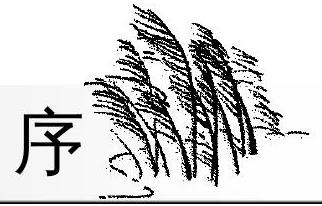
\includegraphics[max width=\textwidth]{2024_10_30_1bf34f7aeb61f11d11d3g-005}
\end{center}

数学竞赛像其他竞赛活动一样,是青少年学生的一种智力竞赛。在类似的以基础科学为竞赛内容的智力竞赛活动中,数学竞赛的历史最悠久、国际性强,影响也最大。我国于1956年开始举行数学竞赛,当时最有威望的著名数学家华罗庚、苏步青、江泽涵等都积极参加领导和组织竞赛活动,并组织出版了一系列青少年数学读物,激励了一大批青年学生立志从事科学事业。我国于1986年起参加国际数学奥林匹克,多次获得团体总分第一,并于1990年在北京成功地举办了第 31 届国际数学奥林匹克,这标志着我国数学竞赛水平在国际上居领先地位,为各国科学家与教育家所瞩目。

我国数学竞赛活动表明,凡是开展好的地区和单位,都能大大激发学生的学习数学的兴趣,有利于培养创造性思维,提高学生的学习效率。这项竞赛活动,将健康的竞争机制引进数学教学过程中,有利于选拔人才。由数学竞赛选拔的优胜者,既有踏实广泛的数学基础,又有刻苦钻研、科学的学习方法,其中的不少青年学生将来会成为出色的科学工作者。在美国,数学竞赛的优胜者中后来成名如米尔诺(J. W. Milnor)、芒福德(D. B. Mumford)、奎伦 (D. Quillen)等都是菲尔兹数学奖的获得者;在波兰,著名数论专家辛哲尔 (A. Schinzel)学生时代是一位数学竞赛优胜者;在匈牙利,著名数学家费叶尔 (L. Fejér)、里斯(M. Riesz)、舍贵(G. Szegö)、哈尔(A. Haar)、拉多 (T. Radó)等都曾是数学竞赛获奖者。匈牙利是开展数学竞赛活动最早的国家,产生了同它的人口不成比例的许多大数学家!

在开展数学竞赛的活动同时,各学校能加强联系,彼此交流数学教学经验,从这种意义上来说,数学竞赛可能成为数学课程改革的"催化剂",成为培养优秀人才的有力措施。

不过,应当注意在数学竞赛活动中,注意普及与提高相结合,而且要以普及为主,使竞赛具有广泛的群众基础,否则难以持久。

当然,现在有些人过于关注数学竞赛的成绩,组织和参与都具有很强的功利目的,过分扩大数学竞赛的作用,这些都是不正确的,违背了开展数学竞赛活动的本意。这些缺点有其深层次的社会原因,需要逐步加以克服,不必因

\section*{001}
为有某些缺点,就否定这项活动。\\
我十分高兴看到这套《数学奥林匹克小丛书》的正式出版。这套书,规模大、专题细。据我所知,这样的丛书还不多见。这套书不仅对数学竞赛中出现的常用方法作了阐述,而且对竞赛题作了精到的分析解答,不少出自作者自己的研究所得, 是一套很好的数学竞赛专题教程, 也是中小学生和教师的参考书。

这套小丛书的作者都是数学竞赛教学和研究人员,不少是国家集训队的教练和国家队的领队。他们为我国开展数学竞赛的活动和我国学生在 IMO 上取得成绩、为国争光作出了贡献,为这套书尽早面世付出了艰辛的劳动。华东师大出版社在出版《奥数教程》和《走向 IMO》等竞赛图书基础上,策划组织了这套丛书,花了不少心血。我非常感谢作者们和编辑们在这方面所做的工作,并衷心祝愿我国的数学竞赛活动开展得越来越好。

\section*{五元}
\footnotetext{王元,著名数学家,中国科学院院士,曾任中国数学会理事长、中国数学奥林匹克委员会主席.
}
1 一次函数的图象与性质 ..... 001\\
2 二次函数的图象与性质 ..... 016\\
3 函数与一元二次方程 ..... 033\\
4 函数与二次不等式 ..... 047\\
5 函数的最值 ..... 059\\
6 有关整数根问题 ..... 072\\
7 函数的应用 ..... 084\\
习题解答 ..... 098\\
001

\section*{华东师大精品奥数图书}
\section*{学奥数,这里总有一本适合你}
"奥数"入门篇——《课本到奥数》(1-9 年级)本书或许不适合你,如果你\\
A. 每次考试都能超过 95 分-so easy!\\
B. 考试很少能超过 80 分一so difficult!\\
C. 不认为自己能学好数学一一Attitude first!读者对象:数学成绩班级前 $5 \%-30 \%$ 的优等生\\
"奥数"智优篇——《优等生数学》(1-9 年级)\\
如果说"奥数"是提供给 $4 \%$ 的优等生,\\
那么《优等生数学》提供给 $20 \%$ 的优等生。\\
如果你已经是优等生,不妨一读;\\
如果你想成为优等生,不能不读!\\
读者对象:数学成绩班级前 $20 \%$ 的优等生\\
"奥数"辅导篇——《奥数教程》、《学习手册》、《能力测试》

\begin{itemize}
  \item 第十届全国教育图书展优秀畅销图书
  \item 国家集训队教练执笔联合编写
  \item 在香港出版繁体字版和网络版
  \item 2010年最新修订,三本配套使用,效果更佳
\end{itemize}

读者对象:数学成绩班级前 $10 \%$ 的优等生、竞赛教练员\\
"奥数"题库篇——《多功能题典》初中、高中数学竞赛

\begin{itemize}
  \item 题量大、内容全、解法精
  \item 分类细:按照章节、难度、题型、方法等维度分类
  \item 配有网络检索功能 \href{http://tidian}{http://tidian}. ecnupress. com. cn读者对象:成绩优秀的中学生、竞赛教练员、数学爱好者\\
"奥数"课外阅读篇——《单墫老师教你学数学》 7 种\\
当读书不只是为了考试\\
你才会真正爱上数学\\
单墫老师妮娓道来\\
与你分享他所理解的数学之美\\
读者对象:初高中学生,数学教师,数学爱好者\\
"奥数"域外篇——《全俄中学生数学奥林匹克(1993-2006)》\\
俄罗斯是世界上开展数学活动最早、最广泛、也是影响最大的国家之一。俄罗斯是世界上竞赛试题的最大生产国,不仅产量高,而且质量好,其中最出色的当数组合题。
\end{itemize}

本书收录 1993-2006年俄罗斯 9-11年级数学奥林匹克第四轮(联邦区域竞赛)和第五轮(全俄决赛)竞赛的所有试题和解答。

读者对象:参加数学竞赛的中学生、竞赛教练员、数学爱好者\\
"奥数"高中预赛篇——《高中数学联赛备考手册(预赛试题集锦)》

\begin{itemize}
  \item 从2009年起,每年出版一册
  \item 收录了当年各省市预赛试题和优秀解答(约 20 份)
  \item 试题在遵循现行教学大纲, 体现新课标精神的同时, 在方法的要求上有所提高
  \item 命题人员大多同时兼任各省市高考命题工作,试题对高考有一定的指导作用\\
读者对象:参加预赛和联赛的高中生、竞赛教练员、高中教师\\
"奥数"联赛冲刺篇——《初(高)中数学联赛考前辅导》
  \item 选题经典且贴近高中联赛
  \item 知识上查漏补缺, 能力上全面提升
  \item 全新模拟题让你提前感受考场氛围
\end{itemize}

读者对象:参加联赛的高中生、竞赛教练员、高中教师\\
"奥数"IMO 终极篇——《走向 IMO:数学奥林匹克试题集锦》

\begin{itemize}
  \item 从 2003 年起,每年出版一册
  \item 以国家集训队测试题和国家队训练题为主
  \item 收集了国内主要竞赛:全国联赛、联赛加试、冬令营、女子数学奥林匹克、西部数学奥林匹克、东南地区数学奥林匹克
  \item 附有美国、俄罗斯、罗马尼亚和国际数学奥林匹克
\end{itemize}

读者对象:参加联赛、冬令营等赛事的高中生、竞赛教练员、数学爱好者\\
更多图书信息及免费资料请登录:\\
\href{http://www}{http://www}. hdsdjf. com/downloadfileinfor. aspx? classid=69

函数 $y=k x+b(k \neq 0)$ 称为一次函数, 若 $b=0$, 则称为正比例函数.\\
一次函数的图象是过 $(0, b) 、\left(-\frac{b}{k}, 0\right)$ 两点的直线。正比例函数 $y=k x$ $(k \neq 0)$ 的图象则是过原点的一条直线. 根据 $k$ 和 $b$ 的符号, 可确定直线经过的象限,如下图所示。\\
(1) $k>0$ 且 $b>0$ 时\\
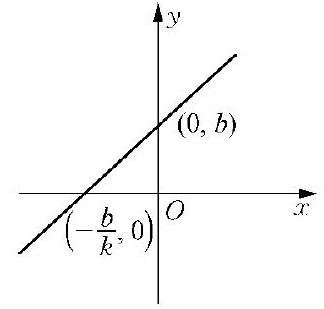
\includegraphics[max width=\textwidth, center]{2024_10_30_1bf34f7aeb61f11d11d3g-010(4)}\\
(4) $k<0$ 且 $b<0$ 时\\
(2) $k>0$ 且 $b<0$ 时\\
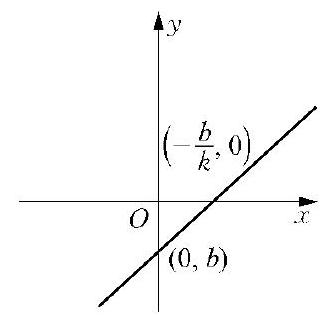
\includegraphics[max width=\textwidth, center]{2024_10_30_1bf34f7aeb61f11d11d3g-010(1)}\\
(3) $k<0$ 且 $b>0$ 时\\
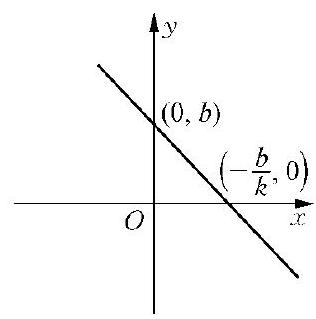
\includegraphics[max width=\textwidth, center]{2024_10_30_1bf34f7aeb61f11d11d3g-010(5)}\\
(5) $k>0$ 且 $b=0$ 时\\
(6) $k<0$ 且 $b=0$ 时\\
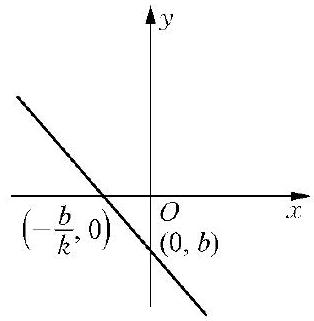
\includegraphics[max width=\textwidth, center]{2024_10_30_1bf34f7aeb61f11d11d3g-010(3)}\\
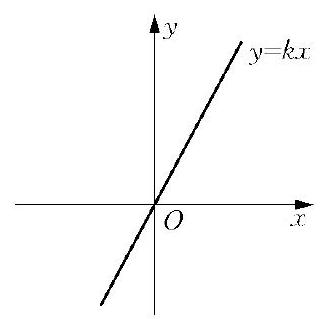
\includegraphics[max width=\textwidth, center]{2024_10_30_1bf34f7aeb61f11d11d3g-010(2)}\\
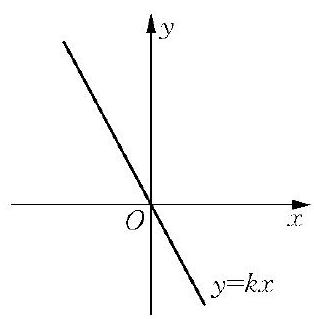
\includegraphics[max width=\textwidth, center]{2024_10_30_1bf34f7aeb61f11d11d3g-010}

由函数的单调性可知,在一次函数 $y=k x+b(k \neq 0)$ 中,当 $k>0$ 时, $y$ 随着 $x$ 的增大而增大,即单调递增;当 $k<0$ 时, $y$ 随着 $x$ 的增大而减小,即单调递减。

另外,正比例函数 $y=k x(k \neq 0)$ 的图象关于原点 $O$ 成中心对称。\\
在解决有关一次函数的问题时,常运用分类讨论和数形结合的思想方法。对分类讨论,在解题过程中,经常分 $k>0$ 或 $k<0$ 等情况进行分步解决. 而对于数形结合,一方面是由数定形,确定图象的大致位置;另一方面是

由形导数, 即从给定的函数图象上获得信息, 确定图象上点的坐标及解析式。

把一次函数解析式 $y=k x+b$ 中的 $y$ 移到右边, 就得到一个关于 $x 、 y$ 的二元一次方程 $k x-y+b=0$, 这时适合一次函数的一组 $x 、 y$ 的值就是相应的二元一次方程的一组解. 因此"一次函数"、"二元一次方程"、"直线"这三个名词有时在不至于引起混淆的情况下通用。

例1 把函数 $y=2 x$ 的图象向右平行移动 3 个单位,求:\\
(1)平移后得到的直线解析式;\\
(2)平移后的直线上到两坐标轴距离相等的点的坐标.\\
解 (1) 因为直线 $y=2 x$ 向右平移 3 个单位, 则平移后经过点 $(3,0)$.\\
设所求解析式为 $y=2 x+b$, 将 $(3,0)$ 代入, 得 $b=-6$.\\
所以所求直线解析式为 $y=2 x-6$.\\
(2) 因为到两坐标轴距离相等的点在直线 $y=x$ 或 $y=-x$ 上, 所以解方程组

\begin{align*}
\begin{gathered}
\left\{\begin{array} { l } 
{ y = 2 x - 6 , } \\
{ y = x , }
\end{array} \text { 和 } \left\{\begin{array}{l}
y=2 x-6, \\
y=-x,
\end{array}\right.\right. \\
x=\begin{array}{l}
x=6, \\
y=6,
\end{array} \text { 和 }\left\{\begin{array}{l}
x=2, \\
y=-2 .
\end{array}\right.
\end{gathered}
\end{align*}

所以在直线 $y=2 x-6$ 上到两坐标轴上的距离相等的点为 $(6,6)$ 和 $(2$, -2 ).

例2 已知 $k=\frac{a+b-c}{c}=\frac{a-b+c}{b}=\frac{-a+b+c}{a}$ ,且 $\sqrt{m+5}+n^{2}+$ $9=6 n$. 问关于自变量 $x$ 的一次函数 $y=k x+m+n$ 的图象一定经过哪几个象限?(黄冈初中数学竞赛)

解 由题意得

\begin{align*}
\left\{\begin{array}{l}
a+b-c=c k \\
a-b+c=b k \\
-a+b+c=a k
\end{array}\right.
\end{align*}

三式相加得

\begin{align*}
(a+b+c)=k(a+b+c)
\end{align*}

当 $a+b+c \neq 0$ 时, $k=1$ ;\\
当 $a+b+c=0$ 时, $k=-2$ 。\\
又由

\begin{align*}
\sqrt{m+5}+n^{2}+9=6 n
\end{align*}

整理得\\
所以\\
则一次函数为\\
或

\begin{align*}
\sqrt{m+5}+(n-3)^{2}=0,
\end{align*}

\begin{align*}
m=-5, n=3,
\end{align*}

\begin{align*}
\begin{gathered}
y=-2 x-2, \\
y=x-2 .
\end{gathered}
\end{align*}

因此,图象一定经过第三、四象限。\\
例3 设 $-1 \leqslant x \leqslant 2$ ,求 $|x-2|-\frac{1}{2}|x|+|x+2|$ 的最大值与最小值之差为多少. (江苏省数学竞赛)

分析 因为 $x$ 的范围为 $-1 \leqslant x \leqslant 2$ ,所以

\begin{align*}
\begin{aligned}
& |x-2|=2-x, \\
& |x+2|=x+2,
\end{aligned}
\end{align*}

而 $|x|$ 不确定,故对 $x$ 分类讨论。\\
解( 1 )当 $-1 \leqslant x<0$ 时,得

\begin{align*}
\begin{aligned}
\text { 原式 } & =2-x+\frac{1}{2} x+x+2 \\
& =\frac{1}{2} x+4,
\end{aligned}
\end{align*}

则最大值为 4 ,最小值为 $\frac{7}{2}$ 。\\
(2)当 $0 \leqslant x \leqslant 2$ 时,得

\begin{align*}
\begin{aligned}
\text { 原式 } & =2-x-\frac{1}{2} x+x+2 \\
& =-\frac{1}{2} x+4,
\end{aligned}
\end{align*}

则最大值为 4 ,最小值为 3 。\\
所以,原式的最大值与最小值之差为 1 。\\
例 4 设 $x$ 是实数,求 $|x+1|+|x+2|+|x+3|+|x+4|+|x+5|$ 的最小值. (北京中学生数学竞赛)

解 根据绝对值的几何意义,在数轴上画出实数 $-1 、-2 、-3 、-4 、-5$ 分别 \begin{tabular}{ccccccc}
$E$ & $D$ & $C$ & $B$ & $P$ & $A$ &  \\
\hline
-5 & -4 & -3 & -2 & $\underset{-1}{1}$ & 0 & $x$ \\
\hline
\end{tabular}对应的点 $A 、 B 、 C 、 D 、 E$, 如图 $1-1$, 设 $x$对应动点 $P$, 则根据绝对值的几何意义, 得

\begin{align*}
\begin{aligned}
& |P A|+|P B|+|P C|+|P D|+|P E| \\
\geqslant & |C B|+|C D|+|C A|+|C E| \\
= & 2+4 \\
= & 6
\end{aligned}
\end{align*}

因此, 当 $x=-3$ 时,取得最小值为 6 .\\
评注 本题也可利用分段函数的图象求解,但相对来说运算较繁琐。\\
一般地,本题还可推广为求 $|x-1|+|x-2|+\cdots+|x-n|(n \in \mathbf{N})$ 的最小值, 则当 $n$ 为偶数且 $\frac{n}{2} \leqslant x \leqslant \frac{n}{2}+1$ 时, 取得最小值为 $\frac{n^{2}}{4}$; 当 $n$ 为奇数且 $x=\frac{n+1}{2}$ 时, 取得最小值为 $\frac{n^{2}-1}{4}$.

例 5 如图 1-2,在平面直角坐标系 $x O y$ 中,多边形 $O A B C D E$ 的顶点坐标分别是 $O(0,0) 、 A$ $(0,6) 、 B(4,6) 、 C(4,4) 、 D(6,4) 、 E(6,0)$ 。若直线 $l$ 经过点 $M(2,3)$ ,且将多边形 $O A B C D E$ 分割成面积相等的两部分,则直线 $l$ 的函数表达式是\\
$\qquad$。\\
解 如图 1-3,延长 $B C$ 交 $x$ 轴于点 $F$ ;连结 $O B, A F$; 连结 $C E, D F$, 且相交于点 $N$. 由已知得\\
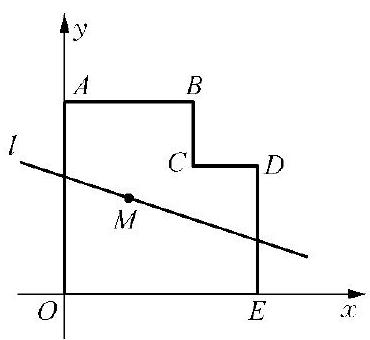
\includegraphics[max width=\textwidth, center]{2024_10_30_1bf34f7aeb61f11d11d3g-013}

图1-2

点 $M(2,3)$ 是 $O B, A F$ 的中点, 即点 $M$ 为矩形 $A B F O$ 的中心,所以直线 $l$ 把矩形 $A B F O$ 分成面积相等的两部分。又因为点 $N(5,2)$ 是矩形 $C D E F$ 的中心,所以,过点 $N(5,2)$ 的直线把矩形 $C D E F$ 分成面积相等的两部分。

于是,直线 $M N$ 即为所求的直线 $l$ 。\\
设直线 $l$ 的函数表达式为 $y=k x+b$ ,则

解得

\begin{align*}
\begin{gathered}
\left\{\begin{array}{l}
2 k+b=3, \\
5 k+b=2,
\end{array}\right. \\
\left\{\begin{array}{l}
k=-\frac{1}{3} \\
b=\frac{11}{3}
\end{array}\right.
\end{gathered}
\end{align*}

\begin{center}
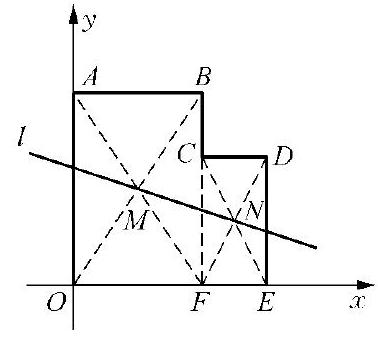
\includegraphics[max width=\textwidth]{2024_10_30_1bf34f7aeb61f11d11d3g-013(1)}
\end{center}

图1-3

故所求直线 $l$ 的函数表达式为 $y=-\frac{1}{3} x+\frac{11}{3}$.\\
例 6 已知一次函数的图象经过点 $(2,2)$ ,它与两坐标轴所围成的三角形

的面积等于 1 ,求这个一次函数的解析式。\\
解 设一次函数为 $y=k x+b$, 它的图象经过点 $(2,2)$, 则点坐标满足函数关系式,得

\begin{align*}
2 k+b=2
\end{align*}

又因为直线 $y=k x+b$ 与 $x$ 轴交于 $\left(-\frac{b}{k}, 0\right)$,与 $y$ 轴交于点 $(0, b)$, 所以三角形面积为

\begin{align*}
S=\frac{1}{2}|b|\left|-\frac{b}{k}\right|=\frac{1}{2} \frac{b^{2}}{|k|}=1,
\end{align*}

即

\begin{align*}
b^{2}=2|k|
\end{align*}

解方程组

得

\begin{align*}
\left\{\begin{array}{l}
2 k+b=2 \\
b^{2}= \pm 2 k
\end{array}\right.
\end{align*}

\begin{align*}
\left\{\begin{array} { l } 
{ k = 2 , } \\
{ b = - 2 , }
\end{array} \text { 或 } \left\{\begin{array}{l}
k=\frac{1}{2}, \\
b=1 .
\end{array}\right.\right.
\end{align*}

所以函数关系式为

\begin{align*}
y=2 x-2 \text { 或 } y=\frac{1}{2} x+1 .
\end{align*}

例 7 甲、 乙两车分别从 $A$ 地将一批物品运往 $B$ 地,再返回 $A$ 地,如图表示两车离 $A$ 地的距离 $s$ (千米) 随时间 $t$ (小时)变化的图象, 已知乙车到达 $B$ 地后以 30 千米/小时的速度返回。请根据图象中的数据回答:\\
(1) 甲车出发多长时间后被乙车追上?\\
(2) 甲车与乙车在距离 $A$ 地多远处迎面相遇?\\
(3) 甲车从 $A$ 地返回的速度多大时, 才能比乙车先回到 $A$ 地?

解 (1) 由图知, 可设甲车由 $A$ 地前往 $B$ 地的函数解析式为 $s=k t$. 将 (2.4, 48) 代入, 解得 $k=20$, 所以 $s=20 t$.

由图可知,在距 $A$ 地 30 千米处,乙车追上甲车,所以当 $s=30$ 千米时, $t=\frac{s}{20}=\frac{30}{20}=1.5$ (小时).

即甲车出发 1.5 小时后被乙车追上.\\
(2)由图知,可设乙车由 $A$ 地前往 $B$ 地函数的解析式为 $s=p t+m$ ,将 $(1.0,0)$ 和 $(1.5,30)$ 代入,得\\
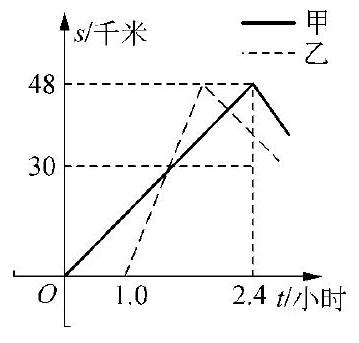
\includegraphics[max width=\textwidth, center]{2024_10_30_1bf34f7aeb61f11d11d3g-014}

图 1-4

\begin{align*}
\left\{\begin{array}{l}
0=p+m \\
30=1.5 p+m
\end{array}\right.
\end{align*}

解得

\begin{align*}
\left\{\begin{array}{l}
p=60, \\
m=-60
\end{array}\right.
\end{align*}

所以 $s=60 t-60$.\\
当乙车到达 $B$ 地时, $s=48$ 千米。代入 $s=60 t-60$ ,得 $t=1.8$ 小时。\\
又设乙车由 $B$ 地返回 $A$ 地的函数的解析式为 $s=-30 t+n$ ,将 $(1.8,48)$代入,得 $48=-30 \times 1.8+n$ ,解得 $n=102$ 。

所以 $s=-30 t+102$.\\
当甲车与乙车迎面相遇时, 有 $-30 t+102=20 t$, 解得 $t=2.04$ 小时, 代入 $s=20 t$ ,得 $s=40.8$ 千米。

即甲车与乙车在距离 $A$ 地 40.8 千米处迎面相遇。\\
(3)当乙车返回到 $A$ 地时,有 $-30 t+102=0$ ,解得 $t=3.4$ 小时。\\
甲车要比乙车先回到 $A$ 地, 速度应大于 $\frac{48}{3.4-2.4}=48$ (千米/时).\\
例 8 已知 $x 、 y 、 z$ 都不小于 0 ,且满足 $3 y+2 z=3-x$ 及 $3 y+z=4-$ $3 x$, 求函数 $u=3 x-2 y+4 z$ 的最大值和最小值.

解 由题意得

由

\begin{align*}
\begin{gathered}
x \geqslant 0, y \geqslant 0, z \geqslant 0 \\
\left\{\begin{array}{l}
3 y+2 z=3-x \\
3 y+z=4-3 x
\end{array}\right.
\end{gathered}
\end{align*}

可得

\begin{align*}
\left\{\begin{array}{l}
y=\frac{5}{3}(1-x) \\
z=2 x-1
\end{array}\right.
\end{align*}

因为要使 $y \geqslant 0 、 z \geqslant 0$, 则可求得

\begin{align*}
\frac{1}{2} \leqslant x \leqslant 1
\end{align*}

又因为

\begin{align*}
\begin{aligned}
u & =3 x-2 y+4 z \\
& =3 x-2\left[\frac{5}{3}(1-x)\right]+4(2 x-1) \\
& =\frac{1}{3}(43 x-22),
\end{aligned}
\end{align*}

所以,当 $x=\frac{1}{2}$ 时, $u$ 取最小值 $-\frac{1}{6}$ ;当 $x=1$ 时, $u$ 取最大值 7 .

例 9 如图 1-5,直线 $y=-x+b(b>0)$ 与双曲线 $y=\frac{k}{x}(k>0)$ 在第一象限的一支分别交于 $A$ 、 $B$ 两点,与坐标轴交于 $C 、 D$ 两点, $P$ 是双曲线上的点,且 $P O=P D$ 。\\
(1)试用 $k 、 b$ 来表示 $C 、 P$ 两点的坐标;\\
(2)若 $\triangle P O D$ 的面积等于 1 ,试求双曲线在第一象限的一支函数解析式;\\
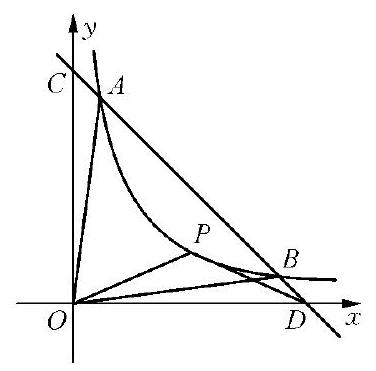
\includegraphics[max width=\textwidth, center]{2024_10_30_1bf34f7aeb61f11d11d3g-016}

图1-5\\
(3)在第(2)小题的结论下,若 $b=4$ ,求 $\triangle A O B$ 的面积。\\
解 (1) 由已知得 $C$ 点坐标为 $(0, b), D$ 点坐标为 $(b, 0)$.\\
又因为 $P O=P D, P$ 点在双曲线 $y=\frac{k}{x}$ 上, 所以 $P$ 点的坐标为 $\left(\frac{b}{2}, \frac{2 k}{b}\right)$.\\
(2)因为

\begin{align*}
S_{\triangle P O D}=1,
\end{align*}

即

\begin{align*}
S_{\triangle P O D}=\frac{1}{2} b \cdot \frac{2 k}{b}=1
\end{align*}

故

\begin{align*}
k=1,
\end{align*}

所以所求函数解析式为 $y=\frac{1}{x}(x>0)$.\\
(3)由题意得

\begin{align*}
\left\{\begin{array}{l}
y=-x+4 \\
y=\frac{1}{x}
\end{array}\right.
\end{align*}

解得

\begin{align*}
\left\{\begin{array} { l } 
{ x = 2 + \sqrt { 3 } , } \\
{ y = 2 - \sqrt { 3 } , \text { 或 } }
\end{array} \left\{\begin{array}{l}
x=2-\sqrt{3}, \\
y=2+\sqrt{3},
\end{array}\right.\right.
\end{align*}

即交点坐标为 $A(2-\sqrt{3}, 2+\sqrt{3}), B(2+\sqrt{3}, 2-\sqrt{3})$, 所以

\begin{align*}
\begin{aligned}
S_{\triangle A O B} & =S_{\triangle A O D}-S_{\triangle B O D} \\
& =\frac{1}{2} \times 4 \times(2+\sqrt{3})-\frac{1}{2} \times 4 \times(2-\sqrt{3}) \\
& =4 \sqrt{3}
\end{aligned}
\end{align*}

例10 设 $a$ 是整数,关于 $x$ 的方程

\begin{align*}
||x-1|-2|=a
\end{align*}

只有三个不同的整数解,求这三个解。\\
解 先作出 $|x-1|$ 的图象,然后向下平移 2 个单位,得到 $|x-1|-2$ 的图象。再把 $x$ 轴下方的图象关于 $x$ 轴翻上去,便得到 $y=||x-1|-2|$ 的图象,如图 1-6.

要使方程只有三个不同的整数解,\\
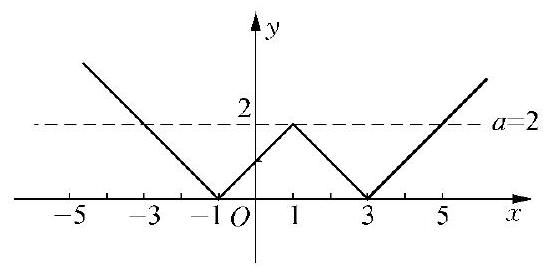
\includegraphics[max width=\textwidth, center]{2024_10_30_1bf34f7aeb61f11d11d3g-017}

图 1-6

只有当 $a=2$ 时成立,即原方程的三个整数解分别为

\begin{align*}
x=-3, x=1, x=5
\end{align*}

评注 本题也可以分区间把函数 $y=||x-1|-2|$ 改写成分段函数,再通过讨论来求解,但有一定的运算量。

例11 已知曲线由方程 $|x-1|+|y-1|=1$ 确定。\\
(1)判别曲线所围成的图形的形状;\\
(2)求所围成的图形的面积。\\
解 (1)根据题意,当 $x \geqslant 1$ 且 $y \geqslant 1$ 时,有

\begin{align*}
x-1+y-1=1,
\end{align*}

即

\begin{align*}
y=-x+3 ;
\end{align*}

当 $x \geqslant 1, y<1$ 时, 有

\begin{align*}
x-1+(1-y)=1
\end{align*}

即

\begin{align*}
y=x-1 \text {; }
\end{align*}

当 $x<1, y \geqslant 1$ 时, 有

\begin{align*}
(1-x)+(y-1)=1,
\end{align*}

即

\begin{align*}
y=x+1 \text {; }
\end{align*}

当 $x<1, y<1$ 时, 有

\begin{align*}
(1-x)+(1-y)=1
\end{align*}

即

\begin{align*}
y=-x+1
\end{align*}

所以,由方程 $|x-1|+|y-1|=1$ 确定的曲线所围成的图形如图 1-7 所示,构成四边形 ABCD.\\
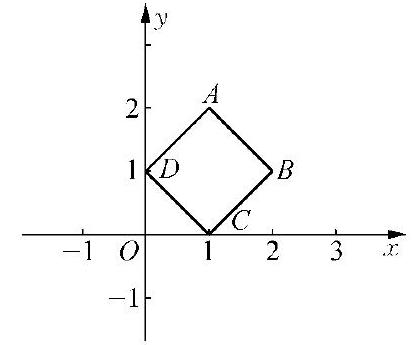
\includegraphics[max width=\textwidth, center]{2024_10_30_1bf34f7aeb61f11d11d3g-017(1)}

图 1-7\\
(2)要求四边形的面积,关键是判定四边形的形状。如图1-7,设直线 $y=-x+3$ 和 $y=x+1$ 交于 $A$ 点, 则 $A$ 点坐标满足

\begin{align*}
\left\{\begin{array}{l}
y=-x+3 \\
y=x+1
\end{array}\right.
\end{align*}

从而求出 $A$ 点坐标为 $(1,2)$.\\
同理可求得 $B(2,1), C(1,0), D(0,1)$.\\
因为

\begin{align*}
\begin{gathered}
A D=\sqrt{(1-0)^{2}+(2-1)^{2}}=\sqrt{2}, \\
A B=C D=C B=\sqrt{2}, \\
D B=2,
\end{gathered}
\end{align*}

且\\
所以

\begin{align*}
A D^{2}+A B^{2}=D B^{2}
\end{align*}

所以四边形 $A B C D$ 为正方形,面积为

\begin{align*}
S_{A B C D}=2
\end{align*}

评注 从本题可以看出,我们在处理有关一次绝对值问题的时候,基本的方法是:(1)分区间进行讨论,把绝对值去掉,然后再分步解决;(2)通过数形结合,画出函数的图象,往往对解题能起到事半功倍的效果。

例12 如图 1-8,直线 $y=2 x+m(m>0)$与 $x$ 轴交于点 $A$ ,直线 $y=-x+n(n>0)$ 与 $x$ 轴、 $y$ 轴分别交于点 $B 、 D$ ,并与直线 $y=2 x+m$ 相交于点 $C$, 若 $A B=4$, 四边形 $C A O D$ 的面积为 $\frac{10}{3}$,求 $m 、 n$ 的值.

分析 要求 $m 、 n$ 两个值,关键找两个关于 $m 、 n$ 的方程。一个是利用 $A B=4$ 这个条件,另一\\
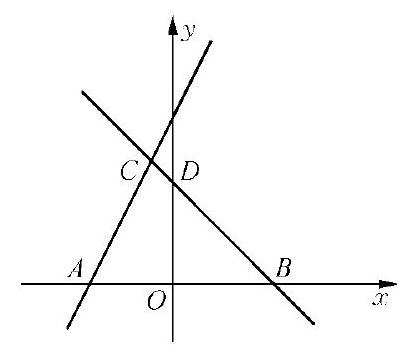
\includegraphics[max width=\textwidth, center]{2024_10_30_1bf34f7aeb61f11d11d3g-018}

图 1-8

个方程利用四边形 $O D C A$ 的面积为 $\frac{10}{3}$ 这个条件。

解 直线 $y=2 x+m$ 与 $x$ 轴的交点 $A\left(-\frac{m}{2}, 0\right)$, 直线 $y=-x+n$ 与 $x$轴的交点为 $B(n, 0)$, 与 $y$ 轴的交点 $D(0, n)$, 则

\begin{align*}
A B=n+\frac{m}{2}=4 \tag{1}
\end{align*}

解方程组

\begin{align*}
\left\{\begin{array}{l}
y=2 x+m \\
y=-x+n
\end{array}\right.
\end{align*}

得

\begin{align*}
\left\{\begin{array}{l}
x=\frac{n-m}{3} \\
y=\frac{m+2 n}{3}
\end{array}\right.
\end{align*}

即 $C$ 点坐标为 $\left(\frac{n-m}{3}, \frac{m+2 n}{3}\right)$.\\
因为

\begin{align*}
\begin{aligned}
& S_{\text {四边形ODCA }} \\
= & S_{\triangle A C B}-S_{\triangle D O B} \\
= & \frac{1}{2} \times 4 \times \frac{m+2 n}{3}-\frac{1}{2} \times n \times n \\
= & \frac{10}{3},
\end{aligned}
\end{align*}

化简后得

\begin{align*}
3 n^{2}-8 n-4 m+20=0 \tag{2}
\end{align*}

联立方程(1)(2),解得

\begin{align*}
\left\{\begin{array}{l}
m=4 \\
n=2
\end{array}\right.
\end{align*}

例13 函数 $y=-\frac{\sqrt{3}}{3} x+1$ 的图象与 $x$ 轴、 $y$ 轴分别交于 $A 、 B$ 两点, $C$点在第一象限内,且 $\triangle A B C$ 是等腰直角三角形, $\angle B A C=90^{\circ}$ ,有一点 $P\left(a, \frac{1}{2}\right)$ 使 $\triangle A B P$ 和 $\triangle A B C$ 的面积相等,求 $a$ 的值.

分析 如图 1 - 9,根据题意,要使 $\triangle A B P$ 和 $\triangle A B C$ 的面积相等, 点 $P$ 应在平行于直线 $A B$ ,且距离等于 $A C$ 的两条平行线上,所以本题关键是求出这两条直线方程。

解 易知 $A$ 点坐标为 $(\sqrt{3}, 0), B$ 点坐标为 $(0,1)$ ,故 $A C=2$ 。\\
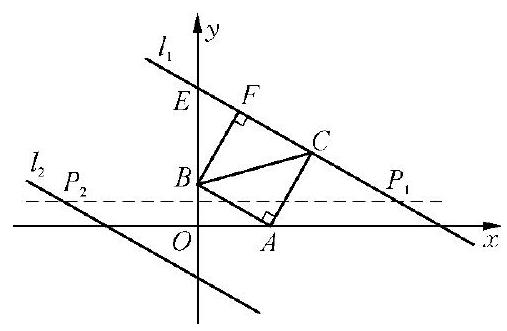
\includegraphics[max width=\textwidth, center]{2024_10_30_1bf34f7aeb61f11d11d3g-019}

图 1 -9

设直线 $l_{1} / / l_{2} / / A B$ ,且 $l_{1}$ 、 $l_{2}$ 到 $A B$ 的距离都等于 $A C$ 。过 $B$ 作 $B F \perp l_{1}$于 $F$ 点, 直线 $l_{1}$ 交 $y$ 轴于 $E$ 点. 易知

所以

\begin{align*}
\begin{gathered}
\angle E B F=30^{\circ}, B F=2, \\
B E=\frac{4 \sqrt{3}}{3},
\end{gathered}
\end{align*}

则直线 $l_{1} 、 l_{2}$ 的方程分别为

\begin{align*}
y=-\frac{\sqrt{3}}{3} x+1+\frac{4 \sqrt{3}}{3} \text { 和 } y=-\frac{\sqrt{3}}{3} x+1-\frac{4 \sqrt{3}}{3} \text {, }
\end{align*}

把 $x=a, y=\frac{1}{2}$, 代入上面两直线方程, 得

\begin{align*}
a=\frac{\sqrt{3}}{2}+4 \text { 或 } a=\frac{\sqrt{3}}{2}-4 \text {. }
\end{align*}

例14 如图 $1-10$ ,直线 $O B$ 是一次函数 $y=$ $2 x$ 的图象,点 $A$ 的坐标为 $(0,2)$ ,在直线 $O B$ 上找点 $C$, 使得 $\triangle A C O$ 为等腰三角形,求点 $C$ 的坐标。

解 分三种情况讨论:\\
(1)若此等腰三角形以 $O A$ 为一腰,且 $A$ 为顶点,则 $A O=A C=2$ 。

设 $C(x, 2 x)$ ,得

\begin{align*}
x^{2}+(2 x-2)^{2}=4,
\end{align*}

\begin{center}
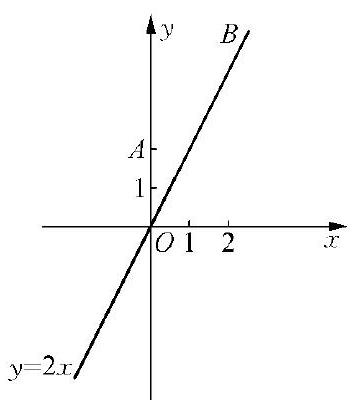
\includegraphics[max width=\textwidth]{2024_10_30_1bf34f7aeb61f11d11d3g-020}
\end{center}

图 1 - 10

解得

\begin{align*}
x=\frac{8}{5} .
\end{align*}

则 $C\left(\frac{8}{5}, \frac{16}{5}\right)$.\\
(2)若此等腰三角形以 $O A$ 为一腰, 且以 $O$ 为顶点, 则 $A O=O C=2$.\\
设 $C(x, 2 x)$ ,得

解得

\begin{align*}
\begin{gathered}
x^{2}+(2 x)^{2}=4, \\
x= \pm \frac{2 \sqrt{5}}{5}
\end{gathered}
\end{align*}

则 $C\left(\frac{2 \sqrt{5}}{5}, \frac{4 \sqrt{5}}{5}\right)$ 或 $C\left(-\frac{2 \sqrt{5}}{5},-\frac{4 \sqrt{5}}{5}\right)$.\\
(3)若等腰三角形以 $O A$ 为底边,则点 $C$ 的纵坐标为 1 , 则横坐标为 $\frac{1}{2}$, 即 $C\left(\frac{1}{2}, 1\right)$.

所以满足题意的 $C$ 有 4 个, 分别为 $C\left(\frac{8}{5}, \frac{16}{5}\right), C\left(\frac{2 \sqrt{5}}{5}, \frac{4 \sqrt{5}}{5}\right)$, $C\left(-\frac{2 \sqrt{5}}{5},-\frac{4 \sqrt{5}}{5}\right)$ 和 $C\left(\frac{1}{2}, 1\right)$.

例 15 已知以 $A(0,2) 、 B(2,0) 、 O(0,0)$ 三点为顶点的三角形被直线 $y=a x-a$ 分成两部分, 设靠近原点 $O$ —侧那部分的面积为 $S$, 试写出用 $a$ 表示的 $S$ 的解析式。

分析 如图 1-11,直线 $y=a x-a$ 是通过定点 $C(1,0)$ 的,在绕着定点 $C(1,0)$ 动的过程中,可能和线段 $O A$ 相交,也可能和线段 $A B$ 相交,则靠近原点 $O$ 一侧的图形可能是三角形,也可能是四边形,故分两种情况讨论。

解 易知直线 $A B$ 的方程为 $y=-x+2(0 \leqslant$ $x \leqslant 2)$ ,直线 $y=a x-a$ 过定点 $C(1,0)$ 。下面分两种情况讨论。\\
(1)直线 $y=a x-a$ 与线段 $O A$ 相交,设交点为 $E$, 则靠近原点 $O$ 一侧的图形是三角形。

在方程 $y=a x-a$ 中,令 $x=0$ ,得 $y=-a>$ 0 ,所以\\
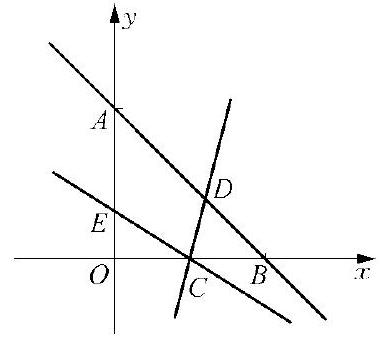
\includegraphics[max width=\textwidth, center]{2024_10_30_1bf34f7aeb61f11d11d3g-021}

图 1-11

\begin{align*}
\begin{aligned}
S & =\frac{1}{2} \times O E \times O C \\
& =\frac{1}{2} \times(-a) \times 1 \\
& =-\frac{a}{2} .
\end{aligned}
\end{align*}

因为 $0<O E \leqslant 2$, 所以 $-2 \leqslant a<0$, 得

\begin{align*}
S=-\frac{a}{2}(-2 \leqslant a<0)
\end{align*}

(2) 直线 $y=a x-a$ 与线段 $A B$ 相交, 设交点为 $D$, 则靠近原点 $O$ 一侧的图形是四边形.由

\begin{align*}
\left\{\begin{array}{l}
y=a x-a \\
y=-x+2
\end{array}\right.
\end{align*}

解得 $D$ 点的坐标为 $\left(\frac{2+a}{1+a}, \frac{a}{1+a}\right)$.\\
所以要求的四边形面积为

即

\begin{align*}
\begin{aligned}
S & =S_{\triangle O A B}-S_{\triangle D C B}, \\
S & =2-\frac{1}{2} \times 1 \times \frac{a}{1+a} \\
& =\frac{4+3 a}{2(1+a)} .
\end{aligned}
\end{align*}

由于点 $D$ 在 $A B$ 上, 所以它的坐标要适合

解得

\begin{align*}
\begin{aligned}
& \left\{\begin{array}{l}
0 \leqslant \frac{2+a}{1+a}<2, \\
0<\frac{a}{1+a} \leqslant 2,
\end{array}\right. \\
& a \leqslant-2 \text { 或 } a>0,
\end{aligned}
\end{align*}

所以

\begin{align*}
S=\frac{4+3 a}{2(1+a)}(a \leqslant-2 \text { 或 } a>0) .
\end{align*}

综合(1)、(2),得

\begin{align*}
S=\left\{\begin{array}{l}
-\frac{a}{2}(-2 \leqslant a<0), \\
\frac{4+3 a}{2(1+a)}(a \leqslant-2 \text { 或 } a>0) .
\end{array}\right.
\end{align*}

\begin{center}
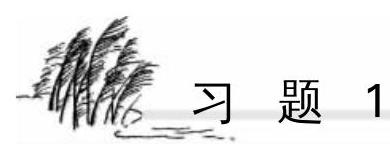
\includegraphics[max width=\textwidth]{2024_10_30_1bf34f7aeb61f11d11d3g-022}
\end{center}

1 有 10 条不同的直线 $y=k_{n} x+b_{n}(n=1,2,3, \cdots, 10)$ ,其中 $k_{3}=k_{6}=$ $k_{9}, b_{4}=b_{7}=b_{10}=0$ ,则这 10 条直线的交点个数最多有 ( ).\\
A. 45 个\\
B. 40 个\\
C. 39 个\\
D. 31 个

2 在一次函数 $y=-x+3$ 图象上取点 $P$ ,作 $P A \perp x$ 轴,垂足为 $A$ ;作 $P B \perp$ $y$ 轴,垂足为 $B$ ;且矩形 $O A P B$ 的面积为 2 ,求点 $P$ 的坐标。\\
3 设 $x 、 y$ 满足 $x+3 y+|3 x-y| \doteq 19,2 x+y=6$ ,求 $x 、 y$ 。\\
4 已知 $|a|=a+1,|x|=2 a x$ ,求 $|x-1|-|x+1|+2$ 的最大值和最小值。\\
5 在平面直角坐标系中,已知直线 $5 x+3 y-15=0$ 分别交 $x$ 轴、 $y$ 轴于 $D$ 、\\
$A$ ,直线 $3 x+5 y-15=0$ 分别交 $x$ 轴、 $y$ 轴于 $B 、 C$ ,且 $A D$ 与 $B C$ 相交于点 $E$,求 $\triangle A B E$ 的面积。\\
6 如图,在直角坐标系中,矩形 $O A B C$ 的顶点 $B$ 的坐标为 $(15,6)$ ,直线 $y=\frac{1}{3} x+b$恰好将矩形 $O A B C$ 分成面积相等的两部分,求 $b$ 的值。\\
7 设关于 $x$ 的一次函数 $y=a_{1} x+b_{1}$ 与 $y=$\\
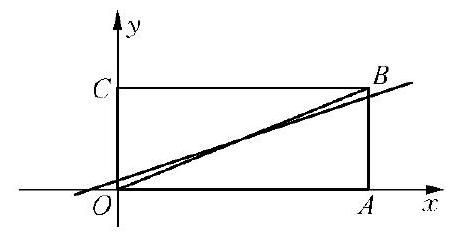
\includegraphics[max width=\textwidth, center]{2024_10_30_1bf34f7aeb61f11d11d3g-022(1)}\\
(第6题)\\
$a_{2} x+b_{2}$, 则称函数 $y=m\left(a_{1} x+b_{1}\right)+n\left(a_{2} x+b_{2}\right)$ (其中 $\left.m+n=1\right)$ 为此两个函数的生成函数。\\
(1)当 $x=1$ 时,求函数 $y=x+1$ 与 $y=2 x$ 的生成函数的值;\\
(2)若函数 $y=a_{1} x+b_{1}$ 与 $y=a_{2} x+b_{2}$ 的图象的交点为 $P$ ,判断点 $P$ 是否在此两个函数的生成函数的图象上,并说明理由。\\
8 如图,在直角坐标系中,已知直角梯形 $O A B C$ 的顶点 $O$ 为坐标原点, $A(3,0), B(2,7), C(0,7) . P$为线段 $O C$ 上一点, 若过 $B 、 P$ 两点的直线为 $y_{1}=$ $k_{1} x+b_{1}$ 过 $A 、 P$ 两点的直线为 $y_{2}=k_{2} x+b_{2}$, 且 $P B \perp P A$ ,求 $k_{1} k_{2}\left(k_{1}+k_{2}\right)$ 的值。\\
9 在直角坐标系 $x O y$ 中,已知 $x$ 轴上的动点 $M(x$, $0)$ 到定点 $Q(5,5) 、 P(2,1)$ 的距离分别为 $M P$ 、 $M Q$, 当点 $M$ 的横坐标为何值时, $M P+M Q$ 的值\\
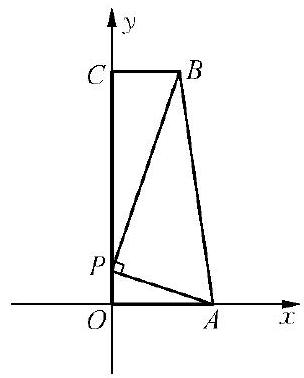
\includegraphics[max width=\textwidth, center]{2024_10_30_1bf34f7aeb61f11d11d3g-023}\\
(第8 题)

最小?\\
10 在直角坐标系中,已知四个点为 $A(-8,3) 、 B(-4,5) 、 C(0, n) 、 D(m$ , 0 ),当四边形 $A B C D$ 的周长最短时,求 $m: n$ 的值。\\
11 如图,已知边长为 1 的正方形 $O A B C$ 在直角坐标系中, $A 、 B$ 两点在第一象限内, $O A$ 与 $x$ 轴的夹角为 $30^{\circ}$, 求点 $B$ 的坐标。\\
$12 A$ 市、 $B$ 市分别有某种库存机器 12 台、 6 台,现决定支援给 $C$ 市 10 台、 $D$ 市 8 台。已知从 $A$ 市调运一台机器到 $C$ 市、 $D$ 市的运费分别为 400 元、 800元;从 $B$ 市调运一台机器到 $C$ 市、 $D$ 市的运费分别为 300 元、 500 元。\\
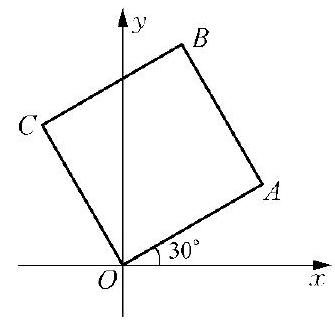
\includegraphics[max width=\textwidth, center]{2024_10_30_1bf34f7aeb61f11d11d3g-023(1)}\\
(第 11 题)\\
(1)设 $B$ 市运往 $C$ 市的机器为 $x$ 台, 求总运费 $w$ 关于 $x$ 的函数关系式;\\
(2)若要求总运费不超过 9000 元,问共有几种调运方案?\\
(3)求出总运费最低的调运方案及最低运费是多少元?\\
13 反比例函数 $y=\frac{5}{x}$ 图象在第一象限的一支上有一点 $C(1,5)$, 过点 $C$ 的直线 $y=-k x+b(k>0)$ 与 $x$ 轴交于点 $A(a, 0)$ 。\\
(1)求点 $A$ 的横坐标 $a$ 与 $k$ 之间的函数关系式;\\
(2)当该直线与反比例函数图象在第一象限的另一交点 $D$ 的横坐标为 9时,求 $\triangle C O A$ 的面积。\\
14 已知一次函数 $y=k_{1} x+b_{1}$ 的图象经过 $(1,6)$ 和( $-3,-2$ )两点,它与 $x$轴、 $y$ 轴的交点分别为 $B 、 A$, 一次函数 $y=k_{2} x+b_{2}$ 的图象经过点 $(2$,\\
$-2)$ ,在 $y$ 轴上的截矩为 -3 ,它与 $x$ 轴、 $y$ 轴的交点分别为 $D 、 C$ 。\\
(1)求这两个一次函数的解析式,并在同一直角坐标系中画出它们的图象;\\
(2) 求四边形 $A B C D$ 的面积;\\
(3) 若直线 $A B 、 C D$ 交于点 $E 、 \triangle B C E$ 和 $\triangle A D E$ 的面积比是多少?

15 已知一次函数 $y=m x+4$ 具有性质: $y$ 随 $x$ 的增大而减小,又直线 $y=$ $m x+4$ 与直线 $x=1 、 x=4$ 分别相交于点 $A 、 D$, 且点 $A$ 在第一象限内,直线 $x=1 、 x=4$ 分别与 $x$ 轴交于点 $B 、 C$.\\
(1)要使四边形 $A B C D$ 为凸四边形,试求 $m$ 的取值范围;\\
(2) 已知四边形 $A B C D$ 为凸四边形,直线 $y=m x+4$ 与 $x$ 轴相交于 $E$ ,且 $\frac{E D}{E A}=\frac{4}{7}$ 时,求一次函数的解析式;\\
(3)在(2)的条件下,直线 $y=m x+4$ 与 $y$ 轴交于点 $F$ ,求证:点 $D$ 是 $\triangle E O F$ 的外心.

\section*{2)}
\section*{二次函数的图象与性质}
\section*{一、二次函数的解析式}
形如 $y=f(x)=a x^{2}+b x+c(a \neq 0)$ 的函数叫做二次函数. 上述解析式称为二次函数的一般形式。

二次函数的标准式(即顶点式)为

\begin{align*}
y=f(x)=a(x-h)^{2}+k(a \neq 0),
\end{align*}

其中 $h$ 、 $k$ 满足 $h=-\frac{b}{2 a}, k=\frac{4 a c-b^{2}}{4 a}$.\\
当二次函数的图象与 $x$ 轴有两个交点 $A\left(x_{1}, 0\right) 、 B\left(x_{2}, 0\right)$ 时,由多项式因式分解可知,二次函数的解析式又可写为

\begin{align*}
y=f(x)=a\left(x-x_{1}\right)\left(x-x_{2}\right)(a \neq 0),
\end{align*}

其中的对称轴方程为 $x=\frac{x_{1}+x_{2}}{2}$, 顶点坐标为 $\left(\frac{x_{1}+x_{2}}{2}, \frac{-a\left(x_{1}-x_{2}\right)^{2}}{4}\right)$.\\
当已知二次函数图象上三点的坐标为 $A\left(x_{1}, f\left(x_{1}\right)\right) 、 B\left(x_{2}, f\left(x_{2}\right)\right)$ 、 $C\left(x_{3}, f\left(x_{3}\right)\right)$ 时,二次函数的解析式为

\begin{align*}
\begin{aligned}
f(x)= & \frac{f\left(x_{1}\right)}{\left(x_{1}-x_{2}\right)\left(x_{1}-x_{3}\right)}\left(x-x_{2}\right)\left(x-x_{3}\right) \\
& +\frac{f\left(x_{2}\right)}{\left(x_{2}-x_{1}\right)\left(x_{2}-x_{3}\right)}\left(x-x_{1}\right)\left(x-x_{3}\right) \\
& +\frac{f\left(x_{3}\right)}{\left(x_{3}-x_{1}\right)\left(x_{3}-x_{2}\right)}\left(x-x_{1}\right)\left(x-x_{2}\right) .
\end{aligned}
\end{align*}

在解题时,可根据条件选择不同的函数形式来解题。

\section*{二、 二次函数的图象与性质}
一元二次函数 $y=f(x)=a x^{2}+b x+c(a \neq 0)$ 的图象是一条抛物线.

当 $a>0$ 时,抛物线的开口向上,图象在区间 $\left(-\infty,-\frac{b}{2 a}\right]$ 上 $y$ 随着 $x$ 的增大而减小(单调递减);图象在区间 $\left[-\frac{b}{2 a},+\infty\right)$ 上 $y$ 随着 $x$ 的增大而增大 (单调递增)。因此,当 $x=-\frac{b}{2 a}$ 时, $f(x)$ 有最小值 $f\left(-\frac{b}{2 a}\right)=\frac{4 a c-b^{2}}{4 a}$.

当 $a<0$ 时,抛物线的开口向下,图象在区间 $\left(-\infty,-\frac{b}{2 a}\right]$ 上 $y$ 随着 $x$ 的增大而增大(单调递增);图象在区间 $\left[-\frac{b}{2 a},+\infty\right)$ 上 $y$ 随着 $x$ 的增大而减小 (单调递减)。因此,当 $x=-\frac{b}{2 a}$ 时, $f(x)$ 有最大值 $f\left(-\frac{b}{2 a}\right)=\frac{4 a c-b^{2}}{4 a}$ 。

解题时,若画抛物线的草图,则要体现抛物线的下列特征:对称轴、顶点位置、开口方向与坐标的交点等。

例1 (1)设抛物线 $y=2 x^{2}$ ,把它向右平移 $p$ 个单位,或向下移 $q$ 个单位,都能使抛物线与直线 $y=x-4$ 恰好有一个交点,求 $p 、 q$ 的值。\\
(2)把抛物线 $y=2 x^{2}$ 向左平移 $p$ 个单位,向上平移 $q$ 个单位,则得到的抛物线经过点( 1,3 )和( 4,9$)$ ,求 $p 、 q$ 的值。\\
(3)把抛物线 $y=a x^{2}+b x+c$ 向左平移 3 个单位,向下平移 2 个单位后,所得抛物线为 $y=a x^{2}$ ,其图象经过点 $\left(-1,-\frac{1}{2}\right)$ ,求原解析式。

解 (1) 抛物线 $y=2 x^{2}$ 向右平移 $p$ 个单位后, 得到 $y=2(x-p)^{2}$. 由

得方程\\
即

\begin{align*}
\left\{\begin{array}{l}
y=2(x-p)^{2} \\
y=x-4
\end{array}\right.
\end{align*}

\begin{align*}
2(x-p)^{2}=x-4,
\end{align*}

\begin{align*}
2 x^{2}-(4 p+1) x+2 p^{2}+4=0
\end{align*}

因为抛物线与直线恰好有一个交点,所以上述方程有两个相同的实数根,故判别式

得

\begin{align*}
\begin{gathered}
\Delta=(4 p+1)^{2}-4 \times 2 \times\left(2 p^{2}+4\right)=0, \\
p=\frac{31}{8},
\end{gathered}
\end{align*}

这时的交点为 $\left(\frac{33}{8}, \frac{1}{8}\right)$.\\
抛物线 $y=2 x^{2}$ 向下平移 $q$ 个单位,得到抛物线 $y=2 x^{2}-q$ ,于是得方程

\begin{align*}
\begin{gathered}
2 x^{2}-q=x-4, \\
2 x^{2}-x+(4-q)=0,
\end{gathered}
\end{align*}

即

该方程有两个相同的实数根,故判别式

\begin{align*}
\Delta=1-4 \times 2 \times(4-q)=0
\end{align*}

得

\begin{align*}
q=\frac{31}{8}
\end{align*}

这时的交点为 $\left(\frac{1}{4},-\frac{15}{4}\right)$.\\
(2)把 $y=2 x^{2}$ 向左平移 $p$ 个单位,向上平移 $q$ 个单位,得到的抛物线为 $y=2(x+p)^{2}+q$. 于是, 由题设得

解得

\begin{align*}
\begin{aligned}
& \left\{\begin{array}{l}
3=2(1+p)^{2}+q, \\
9=2(4+p)^{2}+q,
\end{array}\right. \\
& \left\{\begin{array}{l}
p=-2, \\
q=1,
\end{array}\right.
\end{aligned}
\end{align*}

即抛物线向右平移了两个单位,向上平移了一个单位。\\
(3)首先,抛物线 $y=a x^{2}$ 经过点 $\left(-1,-\frac{1}{2}\right)$ ,可求得 $a=-\frac{1}{2}$ ,设原来的二次函数为

\begin{align*}
y=-\frac{1}{2}(x-h)^{2}+k,
\end{align*}

可得

\begin{align*}
\left\{\begin{array}{l}
-h+3=0, \\
k-2=0
\end{array}\right.
\end{align*}

解得

\begin{align*}
\left\{\begin{array}{l}
h=3 \\
k=2
\end{array}\right.
\end{align*}

所以原二次函数为

\begin{align*}
y=-\frac{1}{2}(x-3)^{2}+2,
\end{align*}

即

\begin{align*}
y=-\frac{1}{2} x^{2}+3 x-\frac{5}{2} .
\end{align*}

说明 将抛物线 $y=a x^{2}+b x+c$ 向右平移 $p$ 个单位,得到的抛物线是 $y=a(x-p)^{2}+b(x-p)+c$ ;向左平移 $p$ 个单位得到 $y=a(x+p)^{2}+b(x+$ $p)+c$ ;向上平移 $q$ 个单位,得到 $y=a x^{2}+b x+c+q$ ;向下平移 $q$ 个单位得到\\
$y=a x^{2}+b x+c-q$.\\
例2 已知二次函数的图象过点 $(3,4)$ ,且在 $x$ 轴上的两个交点为( 1 , $0),(-2,0)$ ,求这个二次函数的解析式。

解法一 设一般式为 $f(x)=a x^{2}+b x+c$, 则由题意知 $f(3)=4, f(1)=$ $f(-2)=0$ ,得方程组

\begin{align*}
\begin{gathered}
9 a+3 b+c=4, \\
a+b+c=0, \\
4 a-2 b+c=0, \\
\left\{\begin{array}{l}
a=\frac{2}{5} \\
b=\frac{2}{5} \\
c=-\frac{4}{5}
\end{array}\right.
\end{gathered}
\end{align*}

所以

\begin{align*}
f(x)=\frac{2}{5} x^{2}+\frac{2}{5} x-\frac{4}{5}
\end{align*}

解法二 设两点式 $f(x)=a(x-1)(x+2)$, 由题设 $f(3)=4$, 则

\begin{align*}
a(3-1)(3+2)=4
\end{align*}

得

\begin{align*}
a=\frac{2}{5}
\end{align*}

所以

\begin{align*}
\begin{aligned}
f(x) & =\frac{2}{5}(x-1)(x+2) \\
& =\frac{2}{5} x^{2}+\frac{2}{5} x-\frac{4}{5}
\end{aligned}
\end{align*}

评注 还可以直接用三点式写出,或者先确定对称轴方程 $x=\frac{1-2}{2}=$ $-\frac{1}{2}$.

例3 设二次函数 $f(x)=a x^{2}+b x+c$ 满足条件: $f(0)=2, f(1)=-1$,且其图象在 $x$ 轴上所截得的线段长为 $2 \sqrt{2}$ 。求这个二次函数的解析式.

解 由 $f(0)=2, f(1)=-1$ ,得

\begin{align*}
\left\{\begin{array}{l}
c=2 \\
a+b+c=-1
\end{array}\right.
\end{align*}

即

\begin{align*}
\left\{\begin{array}{l}
c=2 \\
b=-(a+3)
\end{array}\right.
\end{align*}

因此

\begin{align*}
f(x)=a x^{2}-(a+3) x+2
\end{align*}

设图象与 $x$ 轴的交点坐标为 $\left(x_{1}, 0\right),\left(x_{2}, 0\right)$, 则

\begin{align*}
\begin{aligned}
2 \sqrt{2} & =\left|x_{1}-x_{2}\right| \\
& =\sqrt{\left(x_{1}+x_{2}\right)^{2}-4 x_{1} x_{2}} \\
& =\sqrt{\left(\frac{a+3}{a}\right)^{2}-4 \times \frac{2}{a}}
\end{aligned}
\end{align*}

整理得

\begin{align*}
7 a^{2}+2 a-9=0
\end{align*}

则

\begin{align*}
a=1 \text { 或 } a=-\frac{9}{7} \text {. }
\end{align*}

所以

\begin{align*}
f(x)=x^{2}-4 x+2
\end{align*}

或者

\begin{align*}
f(x)=-\frac{9}{7} x^{2}-\frac{12}{7} x+2
\end{align*}

例 4 已知抛物线 $y=a x^{2}+b x+c$ 的一段图象如图 2-1 所示.\\
(1)确定 $a 、 b 、 c$ 的符号;\\
(2)求 $a+b+c$ 的取值范围.\\
解 (1)由抛物线开口向上,所以 $a>0$ 。又抛物线经过点 $(0,-1)$, 所以 $c=-1<0$ 。因为抛物线的对称轴在 $y$ 轴的右侧,从而 $-\frac{b}{2 a}>0$ ,结合 $a>0$ 便可知 $b<0$ 。

所以 $a>0, b<0, c<0$.\\
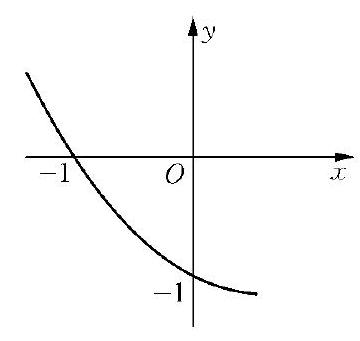
\includegraphics[max width=\textwidth, center]{2024_10_30_1bf34f7aeb61f11d11d3g-029}

图2-1\\
(2) 设 $f(x)=a x^{2}+b x+c$, 由图象及 (1) 可知

\begin{align*}
\left\{\begin{array}{l}
f(-1)=a-b+c=0, \\
a>0 \\
b<0 \\
c=-1
\end{array}\right.
\end{align*}

即

\begin{align*}
\left\{\begin{array}{l}
a-b=1 \\
b<a<1 \\
-1<b<0 \\
c=-1
\end{array}\right.
\end{align*}

因为

\begin{align*}
\begin{aligned}
& a+b+c \\
= & (b+1)+b-1 \\
= & 2 b,
\end{aligned}
\end{align*}

所以

\begin{align*}
-2<a+b+c<0
\end{align*}

例 5 已知两个二次函数 $y_{1}$ 和 $y_{2}$, 当 $x=a(a>0)$ 时, $y_{1}$ 取得最大值 5 ,且 $y_{2}=25$, 又 $y_{2}$ 的最小值为 $-2, y_{1}+y_{2}=x^{2}+16 x+13$. 求 $a$ 的值及二次函数 $y_{1} 、 y_{2}$ 的解析式. (全国初中数学竞赛天津赛区初赛)

解 设 $y_{1}=m(x-a)^{2}+5$ ,则

\begin{align*}
y_{2}=x^{2}+16 x+13-m(x-a)^{2}-5 .
\end{align*}

又因为当 $x=a$ 时, $y_{2}=25$, 即

\begin{align*}
a^{2}+16 a+8=25,
\end{align*}

解得

\begin{align*}
a_{1}=1 \text { 或 } a_{2}=-17 \text { (舍去), }
\end{align*}

故

\begin{align*}
\begin{aligned}
y_{2} & =x^{2}+16 x+13-m(x-1)^{2}-5 \\
& =(1-m) x^{2}+(16+2 m) x+(8-m)
\end{aligned}
\end{align*}

因为 $y_{2}$ 的最小值为 -2 , 所以有

\begin{align*}
\frac{4(1-m)(8-m)-4(8+m)^{2}}{4(1-m)}=-2
\end{align*}

解得

\begin{align*}
m=-2
\end{align*}

所以

\begin{align*}
\begin{aligned}
& y_{1}=-2 x^{2}+4 x+3 \\
& y_{2}=3 x^{2}+12 x+10
\end{aligned}
\end{align*}

例 6 证明:无论 $a$ 取何实数值,抛物线 $y=x^{2}+(a+1) x+\frac{1}{2} a+\frac{1}{4}$ 恒过定点,而且这些抛物线的顶点都在一条确定的抛物线上.

证明 由

\begin{align*}
\begin{aligned}
y & =x^{2}+(a+1) x+\frac{1}{2} a+\frac{1}{4} \\
& =x^{2}+x+\frac{1}{4}+a\left(x+\frac{1}{2}\right) \\
& =\left(x+\frac{1}{2}\right)^{2}+a\left(x+\frac{1}{2}\right)
\end{aligned}
\end{align*}

可知,当 $x=-\frac{1}{2}$ 时, $y=0$ ,即抛物线恒过定点 $\left(-\frac{1}{2}, 0\right)$.\\
下面求抛物线的顶点:\\
因为

\begin{align*}
\begin{aligned}
y & =x^{2}+(a+1) x+\frac{1}{2} a+\frac{1}{4} \\
& =\left(x+\frac{a+1}{2}\right)^{2}-\frac{1}{4} a^{2}
\end{aligned}
\end{align*}

所以抛物线的顶点坐标为 $\left(-\frac{a+1}{2},-\frac{1}{4} a^{2}\right)$, 即有

\begin{align*}
\left\{\begin{array}{l}
x=-\frac{a+1}{2} \\
y=-\frac{1}{4} a^{2}
\end{array}\right.
\end{align*}

消去变量 $a$ ,就得到

\begin{align*}
y=-\left(x+\frac{1}{2}\right)^{2}=-x^{2}-x-\frac{1}{4}
\end{align*}

这说明原抛物线的顶点都在一条确定的抛物线 $y=-x^{2}-x-\frac{1}{4}$ 上.\\
例7 当 $n=1,2, \cdots, 2012$ 时,求所有二次函数 $y=\left(n^{2}+n\right) x^{2}-(2 n+$ 1) $x+1$ 的图象与 $x$ 轴所截得的线段长度之和。

解 二次函数的解析式用两点式表示为

\begin{align*}
y=n \cdot(n+1)\left(x-\frac{1}{n+1}\right)\left(x-\frac{1}{n}\right),
\end{align*}

则它与 $x$ 轴两交点为

\begin{align*}
\left(\frac{1}{n+1}, 0\right),\left(\frac{1}{n}, 0\right)
\end{align*}

所截线段长度为

\begin{align*}
\begin{aligned}
d_{n} & =\left|\frac{1}{n+1}-\frac{1}{n}\right| \\
& =\frac{1}{n}-\frac{1}{n+1}(n=1,2, \cdots, 2012)
\end{aligned}
\end{align*}

所以

\begin{align*}
\begin{aligned}
& d_{1}+d_{2}+\cdots+d_{2012} \\
= & \left(\frac{1}{1}-\frac{1}{2}\right)+\left(\frac{1}{2}-\frac{1}{3}\right)+\cdots+\left(\frac{1}{2012}-\frac{1}{2013}\right)
\end{aligned}
\end{align*}

\begin{align*}
\begin{aligned}
& =1-\frac{1}{2013} \\
& =\frac{2012}{2013}
\end{aligned}
\end{align*}

例8 当二次函数 $f(x)=a(x-m)^{2}+n,(a \neq 0)$ 与 $x$ 轴的两交点和函数图象的顶点所围成的三角形为顶角是 $120^{\circ}$ 的等腰三角形时, 求 $a 、 n$ 应满足的关系式。

解 设二次函数 $f(x)=a(x-m)^{2}+n$ 与 $x$ 轴的两交点分别为 $A 、 B$, 顶点为 $C$ ,过 $C$ 作 $x$ 轴的垂线交于点 $D$ ,要使所围成的 $\triangle A B C$ 为有一个角为 $120^{\circ}$的等腰三角形, 则 $\angle A=30^{\circ}, A C=2 C D, A B=2 \sqrt{3} C D, A D=\sqrt{3} C D$, 且 $a n<0$ 。

又因为 $C$ 点纵坐标为 $n$, 所以 $f(x)$ 与 $x$ 轴交于点 $(m \pm \sqrt{3} n, 0)$, 因而

\begin{align*}
\begin{gathered}
a(m \pm \sqrt{3} n-m)^{2}+n=0 \\
3 a n^{2}+n=0
\end{gathered}
\end{align*}

则\\
当 $n=0$ 时, 不符合题意, 所以 $3 a n=-1$.\\
故当 $3 a n=-1$ 时,二次函数 $f(x)=a(x-m)^{2}+n$ 与 $x$ 轴的两交点和顶点所围成的三角形为有一个角为 $120^{\circ}$ 的等腰三角形。

例 9 已知二次函数的图象开口向上且不过原点 $O$, 顶点坐标为 $(1,-2)$ ,与 $x$ 轴交于点 $A 、 B$ ,与 $y$ 轴交于点 $C$ ,且满足关系式 $|O C|^{2}=|O A| \cdot|O B|$ 。\\
(1)求二次函数解析式;\\
(2)求 $\triangle A B C$ 的面积。(太原初中数学竞赛)\\
解 设二次函数的解析式为

即

\begin{align*}
\begin{gathered}
y=a(x-1)^{2}-2, \\
y=a x^{2}-2 a x+a-2,
\end{gathered}
\end{align*}

其中 $a>0, a \neq 2$ ,图象如图 2-2 所示。\\
设图象与 $x$ 轴的交点为 $A\left(x_{1}, 0\right)$ 和 $B\left(x_{2}, 0\right)$,图象与 $y$ 轴的交点为 $C(0, a-2)$ 。\\
(1) 由 $|O C|^{2}=|O A| \cdot|O B|$,

得

\begin{align*}
(a-2)^{2}=\left|x_{1} x_{2}\right|=\left|\frac{a-2}{a}\right|
\end{align*}

当 $a>2$ 时, 原式化为\\
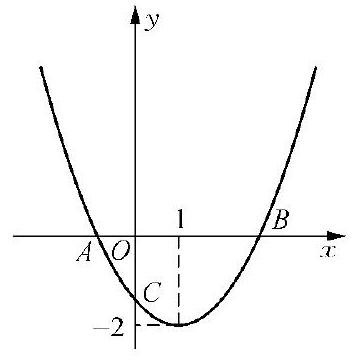
\includegraphics[max width=\textwidth, center]{2024_10_30_1bf34f7aeb61f11d11d3g-032}

图2-2

\begin{align*}
a(a-2)=1,
\end{align*}

解得

\begin{align*}
a=1+\sqrt{2} \text { 或 } a=1-\sqrt{2}<0 \text { (舍去); }
\end{align*}

当 $0<a<2$ 时, 原式化为

\begin{align*}
a(a-2)=-1,
\end{align*}

解得

\begin{align*}
a=1
\end{align*}

因此,函数解析式为

\begin{align*}
y=x^{2}-2 x-1,
\end{align*}

或

\begin{align*}
y=(1+\sqrt{2}) x^{2}-(2+2 \sqrt{2}) x+\sqrt{2}-1 .
\end{align*}

(2)由 $S_{\triangle A B C}=\frac{1}{2}|A B||O C|$ ,分以下两种情况讨论:\\
当 $y=x^{2}-2 x-1$ 时,因为

\begin{align*}
|A B|=\sqrt{\left(x_{1}+x_{2}\right)^{2}-4 x_{1} x_{2}}=2 \sqrt{2},
\end{align*}

又

\begin{align*}
|O C|=1
\end{align*}

所以

\begin{align*}
S_{\triangle A B C}=\frac{1}{2} \times 2 \sqrt{2} \times 1=\sqrt{2}
\end{align*}

当 $y=(1+\sqrt{2}) x^{2}-(2+2 \sqrt{2}) x+\sqrt{2}-1$ 时,因为

又

\begin{align*}
\begin{aligned}
|A B| & =\sqrt{\left(x_{1}+x_{2}\right)^{2}-4 x_{1} x_{2}} \\
& =2 \sqrt{2(\sqrt{2}-1)}
\end{aligned}
\end{align*}

\begin{align*}
|O C|=\sqrt{2}-1,
\end{align*}

所以

\begin{align*}
\begin{aligned}
S_{\triangle A B C} & =\frac{1}{2} \times 2 \sqrt{2(\sqrt{2}-1)} \times(\sqrt{2}-1) \\
& =(\sqrt{2}-1) \sqrt{2(\sqrt{2}-1)} .
\end{aligned}
\end{align*}

故所求 $\triangle A B C$ 的面积为 $\sqrt{2}$ 或 $(\sqrt{2}-1) \sqrt{2(\sqrt{2}-1)}$.\\
例10 已知二次函数 $y=a x^{2}+b x+c$ (其中 $a$ 是正整数)的图象经过点\\
$A(-1,4)$ 和 $B(2,1)$ ,且与 $x$ 轴有两个不同的交点,求 $b+c$ 的最大值。\\
解 由函数经过点 $A(-1,4), B(2,1)$ ,则有

\begin{align*}
\left\{\begin{array}{l}
a-b+c=4, \\
4 a+2 b+c=1
\end{array}\right.
\end{align*}

解得

\begin{align*}
\left\{\begin{array}{l}
b=-a-1 \\
c=3-2 a
\end{array}\right.
\end{align*}

因为二次函数与 $x$ 轴有两个不同交点,则

\begin{align*}
\Delta=b^{2}-4 a c>0
\end{align*}

即

\begin{align*}
(-a-1)^{2}-4 a(3-2 a)>0
\end{align*}

整理为

\begin{align*}
(9 a-1)(a-1)>0,
\end{align*}

解得

\begin{align*}
a<\frac{1}{9} \text { 或 } a>1 .
\end{align*}

由于 $a$ 为正整数,所以 $a \geqslant 2$ 。\\
又因为 $b+c=-3 a+2 \leqslant-4$ ,且当 $a=2 、 b=-3 、 c=-1$ 时,满足题意,故 $b+c$ 的最大值为 -4 。

例11 某学生为了通过描点作出函数 $y=a x^{2}+b x+c(a \neq 0)$ 的图象,先取自变量 $x$ 的 7 个值满足 $x_{1}<x_{2}<\cdots<x_{7}$ ,且 $x_{2}-x_{1}=x_{3}-x_{2}=\cdots=$ $x_{7}-x_{6}$ ,再分别算出对应的 $y$ 值,列出表 1.

表 1

\begin{center}
\begin{tabular}{c|c|c|c|c|c|c|c}
\hline
$x$ & $x_{1}$ & $x_{2}$ & $x_{3}$ & $x_{4}$ & $x_{5}$ & $x_{6}$ & $x_{7}$ \\
\hline
$y$ & 51 & 107 & 185 & 285 & 407 & 549 & 717 \\
\hline
\end{tabular}
\end{center}

但由于粗心算错了其中的一个 $y$ 值,请指出算错的是哪一个值?正确的值是多少?并说明理由。(上海初中数学竞赛)

解 设 $x_{2}-x_{1}=x_{3}-x_{2}=\cdots=x_{7}-x_{6}=d$ ,且 $x_{i}$ 对应的函数值为 $y_{i}$ ,则

\begin{align*}
\begin{aligned}
\Delta_{k} & =y_{k+1}-y_{k} \\
& =\left(a x_{k+1}^{2}+b x_{k+1}+c\right)-\left(a x_{k}^{2}+b x_{k}+c\right) \\
& =a\left[\left(x_{k}+d\right)^{2}-x_{k}^{2}\right]+b\left[\left(x_{k}+d\right)-x_{k}\right] \\
& =2 a d x_{k}+a d^{2}+b d
\end{aligned}
\end{align*}

故

\begin{align*}
\begin{aligned}
\Delta_{k+1}-\Delta_{k} & =2 a d\left(x_{k+1}-x_{k}\right) \\
& =2 a d^{2}(\text { 常数 }) .
\end{aligned}
\end{align*}

由给出的数据,可得\\
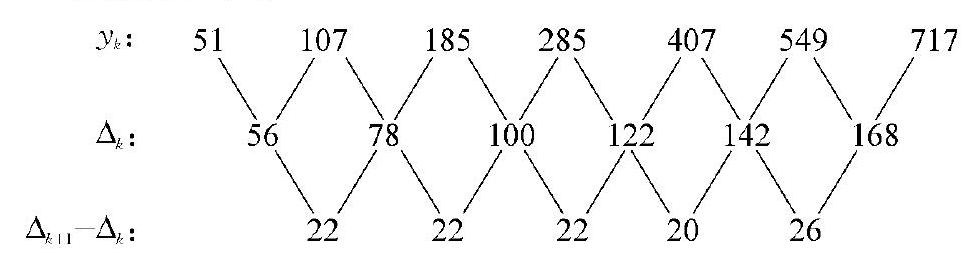
\includegraphics[max width=\textwidth, center]{2024_10_30_1bf34f7aeb61f11d11d3g-034}

由此可见, 549 是被算错的 $y$ 值,其正确值应为 551 。\\
例12 设二次函数 $f(x)=a x^{2}+b x+c(a>0)$ ,方程 $f(x)=x$ 的根为 $x_{1} 、 x_{2}$ ,且 $x_{2}-x_{1}>\frac{1}{a}$ ,当 $0<t<x_{1}$ 时,试比较 $f(t)$ 与 $x_{1}$ 的大小关系。

解法一 已知方程 $f(x)=x$ ,整理为

\begin{align*}
a x^{2}+(b-1) x+c=0 .
\end{align*}

由韦达定理得

\begin{align*}
\left\{\begin{array}{l}
x_{1}+x_{2}=-\frac{b-1}{a}, \\
x_{1} x_{2}=\frac{c}{a},
\end{array}\right.
\end{align*}

根据题意 $a>0$, 则

所以

\begin{align*}
\begin{gathered}
x_{2}-x_{1}>\frac{1}{a}>0, \\
x_{2}-x_{1}=\frac{\sqrt{(b-1)^{2}-4 a c}}{a}>\frac{1}{a},
\end{gathered}
\end{align*}

得到

\begin{align*}
\sqrt{(b-1)^{2}-4 a c}>1 . \tag{*}
\end{align*}

又 $x_{1}$ 是方程 $f(x)=x$ 的根, 则

\begin{align*}
x_{1}=\frac{-(b-1)-\sqrt{(1-b)^{2}-4 a c}}{2 a},
\end{align*}

由(*)可知

\begin{align*}
\begin{aligned}
x_{1} & <\frac{-(b-1)-1}{2 a} \\
& =-\frac{b}{2 a} .
\end{aligned}
\end{align*}

又因为 $f(x)$ 开口向上, 在 $\left(-\infty,-\frac{b}{2 a}\right]$ 是单调递减的, 且由题意

\begin{align*}
0<t<x_{1}<-\frac{b}{2 a}
\end{align*}

因此

\begin{align*}
f(t)>f\left(x_{1}\right)=x_{1} .
\end{align*}

解法二 由已知方程 $f(x)=x$ 的两根为 $x_{1} 、 x_{2}$, 则有

\begin{align*}
f(x)-x=a\left(x-x_{1}\right)\left(x-x_{2}\right),
\end{align*}

即

\begin{align*}
f(x)=a\left(x-x_{1}\right)\left(x-x_{2}\right)+x .
\end{align*}

因为

\begin{align*}
\begin{aligned}
& f(t)-x_{1} \\
= & a\left(t-x_{1}\right)\left(t-x_{2}\right)+t-x_{1} \\
= & \left(t-x_{1}\right)\left[a\left(t-x_{2}\right)+1\right],
\end{aligned}
\end{align*}

由题意

\begin{align*}
0<t<x_{1},
\end{align*}

得

\begin{align*}
t-x_{1}<0 \tag{1}
\end{align*}

又由

\begin{align*}
x_{2}-x_{1}>\frac{1}{a},
\end{align*}

可得

\begin{align*}
\begin{gather*}
x_{2}-t>\frac{1}{a}, \\
a\left(x_{2}-t\right)>1, \\
a\left(t-x_{2}\right)<-1, \\
a\left(t-x_{2}\right)+1<0,
\end{gather*} \tag{2}
\end{align*}

综合(1)(2), 有 $f(t)-x_{1}>0$ ,所以 $f(t)>x_{1}$ 。\\
评注 题目要求比较 $f(t)$ 与 $x_{1}$ 的大小, 解法一是去比较 $f(t)$ 与 $f\left(x_{1}\right)$ 的大小关系,利用不等式得到 $0<t<x_{1}<-\frac{b}{2 a}$ ,从而解决此题。而解法二是利用已知二次方程的两根,把函数 $f(x)$ 写成 $a\left(x-x_{1}\right)\left(x-x_{2}\right)+x$ 的形式,通过作差比较来解决此题的。

例13 已知抛物线 $C_{1}: y=a x^{2}-2 a m x+a m^{2}+2 m+1(a>0, m>0)$的顶点为 $A$, 抛物线 $C_{2}$ 的顶点 $B$ 在 $y$ 轴上, 且抛物线 $C_{1}$ 和 $C_{2}$ 关于 $P(1,3)$成中心对称。\\
(1)当 $a=1$ 时,求抛物线 $C_{2}$ 的解析式和 $m$ 的值;\\
(2)设抛物线 $C_{2}$ 与 $x$ 轴正半轴的交点是 $C$, 当 $\triangle A B C$ 为等腰三角形时,求 $a$ 的值。

解 (1) 当 $a=1$ 时, 因为 $y=x^{2}-2 m x+m^{2}+2 m+1=(x-m)^{2}+$ $2 m+1$, 所以顶点 $A(m, 2 m+1)$.

设抛物线 $C_{2}$ 的顶点 $B\left(0, y_{B}\right)$, 又因为抛物线 $C_{1}$ 和 $C_{2}$ 关于 $P(1,3)$ 成中心对称,则有

\begin{align*}
\left\{\begin{array}{l}
\frac{m+0}{2}=1, \\
\frac{2 m+1+y_{B}}{2}=3,
\end{array}\right.
\end{align*}

解得

\begin{align*}
\left\{\begin{array}{l}
m=2 \\
y_{B}=1
\end{array}\right.
\end{align*}

即抛物线 $C_{2}$ 的顶点 $B(0,1)$, 又 $C_{1}$ 和 $C_{2}$ 的开口大小相同, 方向相反, 则 $C_{2}$ 的解析式为 $y=-x^{2}+1$.

所以 $C_{2}$ 的解析式为 $y=-x^{2}+1, m$ 值为 2 .\\
(2) 由第 (1) 小题知: 抛物线 $C_{1}$ 的顶点为 $A(2,5)$, 抛物线 $C_{2}$ 的顶点为 $B(0,1)$, 且抛物线 $C_{2}$ 的解析式为 $y=-a x^{2}+1$, 设 $C(n, 0)$, 现要使 $\triangle A B C$为等腰三角形,则有\\
(1) 若 $A B=A C$, 得

\begin{align*}
\begin{aligned}
& A B=\sqrt{2^{2}+4^{2}}=2 \sqrt{5} \\
& A C=\sqrt{(n-2)^{2}+25}
\end{aligned}
\end{align*}

易知无解;\\
(2) 若 $A B=B C$ ,得

\begin{align*}
\begin{gathered}
A B=2 \sqrt{5}, \\
B C=\sqrt{n^{2}+1}, \\
n=\sqrt{19} .
\end{gathered}
\end{align*}

所以 $a=\frac{1}{19}$ ;\\
(3) 若 $A C=B C$, 得

\begin{align*}
\begin{gathered}
A C=\sqrt{(n-2)^{2}+25}, \\
B C=\sqrt{n^{2}+1}, \\
n=7 .
\end{gathered}
\end{align*}

解得\\
所以 $a=\frac{1}{49}$.\\
综上, 满足 $\triangle A B C$ 为等腰三角形的 $a$ 的值有 $a=\frac{1}{19}$ 或 $a=\frac{1}{49}$.\\
例14 已知 $a 、 b 、 c$ 是实数, 函数 $f(x)=a x^{2}+b x+c, g(x)=a x+b$,当 $-1 \leqslant x \leqslant 1$ 时, $|f(x)| \leqslant 1$ 。\\
(1)证明: $|c| \leqslant 1$ ;\\
(2)证明:当 $-1 \leqslant x \leqslant 1$ 时, $|g(x)| \leqslant 2$ ;\\
(3)设 $a>0$ ,当 $-1 \leqslant x \leqslant 1$ 时, $g(x)$ 的最大值为 2 ,求 $f(x)$ 的表达式。

解 (1)因为当 $-1 \leqslant x \leqslant 1$ 时, $|f(x)| \leqslant 1$ ,所以

\begin{align*}
|c|=|f(0)| \leqslant 1
\end{align*}

(2)因为 $g(x)=a x+b$ 是一次函数,则在 $-1 \leqslant x \leqslant 1$ 上的图象是一条线段, 所以 $g(x)$ 的最大值在 $g(1)$ 或 $g(-1)$ 上取到, 则

\begin{align*}
\begin{aligned}
|g(1)| & =|a+b|=|a+b+c-c| \\
& =|f(1)-f(0)| \\
& \leqslant|f(1)|+|f(0)| \\
& \leqslant 1+1 \\
& \leqslant 2 .
\end{aligned}
\end{align*}

同理

\begin{align*}
\begin{aligned}
|g(-1)| & =|a-b|=|a-b+c-c| \\
& =|f(-1)-f(0)| \\
& \leqslant|f(-1)|+|f(0)| \\
& \leqslant 2 .
\end{aligned}
\end{align*}

所以 $|g(x)| \leqslant 2$.\\
(3)因为当 $a>0$ 时, $g(x)$ 在 $[-1,1]$ 上是单调递增的,则有

又因为

\begin{align*}
a+b=2
\end{align*}

\begin{align*}
\begin{aligned}
f(1) & =a+b+c \\
& =2+c \leqslant 1,
\end{aligned}
\end{align*}

得到

\begin{align*}
c \leqslant-1,
\end{align*}

根据第 (1) 小题 $-1 \leqslant c \leqslant 1$, 则有

\begin{align*}
c=-1,
\end{align*}

所以 $f(x)$ 在 $[-1,1]$ 上的最小值为 $f(0)=-1$ ,根据二次函数图象,函数的对称轴只能是 $y$ 轴,即

由

\begin{align*}
\begin{gathered}
b=0 \\
a+b=2
\end{gathered}
\end{align*}

得

\begin{align*}
a=2,
\end{align*}

所以

\begin{align*}
f(x)=2 x^{2}+1
\end{align*}

例15 如图 2-3,抛物线 $y=a x^{2}+b x(a>0)$ 与双曲线 $y=\frac{k}{x}$ 相交于点 $A 、 B$. 已知点 $A$ 的坐标为 $(1,4)$, 点 $B$ 在第三象限内, 且 $\triangle A O B$ 的面积为 3\\
( $O$ 为坐标原点)。\\
(1) 求实数 $a 、 b 、 k$ 的值;\\
(2)过抛物线上点 $A$ 作直线 $A C / / x$ 轴,交抛物线于另一点 $C$ ,求所有满足 $\triangle E O C \backsim \triangle A O B$的点 $E$ 的坐标。\\
(其中点 $E$ 和点 $A$ ,点 $C$ 和点 $B$ 分别是对应点)

解 (1)因为点 $A(1,4)$ 在双曲线 $y=\frac{k}{x}$\\
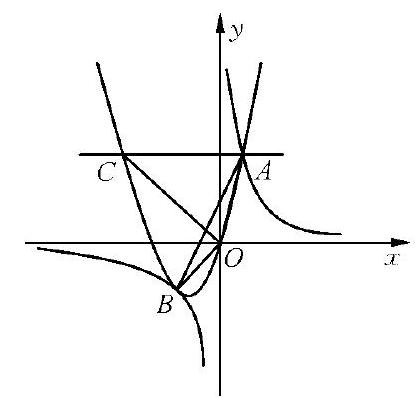
\includegraphics[max width=\textwidth, center]{2024_10_30_1bf34f7aeb61f11d11d3g-039(1)}

图2-3

上, 所以 $k=4$.

故双曲线的函数表达式为 $y=\frac{4}{x}$ ,设点 $B\left(t, \frac{4}{t}\right), t<0$ 。\\
$A B$ 所在直线的函数表达式为 $y=m x+n$, 则有

\begin{align*}
\left\{\begin{array}{l}
4=m+n \\
\frac{4}{t}=m t+n
\end{array}\right.
\end{align*}

解得

\begin{align*}
m=-\frac{4}{t}, n=\frac{4(t+1)}{t}
\end{align*}

于是, 直线 $A B$ 与 $y$ 轴的交点坐标为 $\left(0, \frac{4(t+1)}{t}\right)$, 故

\begin{align*}
S_{\triangle A O B}=\frac{1}{2} \times \frac{4(t+1)}{t}(1-t)=3
\end{align*}

整理得 $2 t^{2}+3 t-2=0$ ,解得 $t=-2$ 或 $t=\frac{1}{2}$ (舍去)。\\
所以点 $B$ 的坐标为 $(-2,-2)$ 。\\
因为点 $A, B$ 都在抛物线 $y=a x^{2}+b x(a>0)$上, 所以 $\left\{\begin{array}{l}a+b=4, \\ 4 a-2 b=-2,\end{array}\right.$ 解得 $\left\{\begin{array}{l}a=1, \\ b=3 .\end{array}\right.$\\
(2)如图2-4, 因为 $A C / / x$ 轴, 所以 $C(-4$, 4),于是 $C O=4 \sqrt{2}$ 。

又 $B O=2 \sqrt{2}$, 所以 $\frac{C O}{B O}=2$.\\
设抛物线 $y=a x^{2}+b x(a>0)$ 与 $x$ 轴负半轴相交于点 $D$, 则点 $D$ 的坐标为 $(-3,0)$ 。

因为 $\angle C O D=\angle B O D=45^{\circ}$, 所以 $\angle C O B=90^{\circ}$.\\
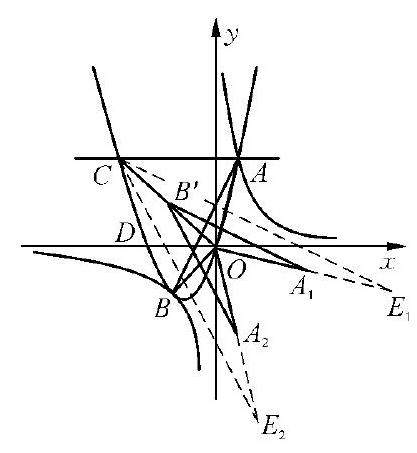
\includegraphics[max width=\textwidth, center]{2024_10_30_1bf34f7aeb61f11d11d3g-039}

图2-4\\
(i) 将 $\triangle B O A$ 绕点 $O$ 顺时针旋转 $90^{\circ}$, 得到 $\triangle B^{\prime} O A_{1}$, 这时点 $B^{\prime}(-2,2)$是 $C O$ 的中点, 点 $A_{1}$ 的坐标为 $(4,-1)$.

延长 $O A_{1}$ 到点 $E_{1}$, 使得 $O E_{1}=2 O A_{1}$, 这时点 $E_{1}(8,-2)$ 是符合条件的点。\\
(ii)作 $\triangle B O A$ 关于 $x$ 轴的对称图形 $\triangle B^{\prime} O A_{2}$ ,得到点 $A_{2}(1,-4)$ ;延长 $O A_{2}$ 到点 $E_{2}$, 使得 $O E_{2}=2 O A_{2}$, 这时点 $E_{2}(2,-8)$ 是符合条件的点.

所以, 点 $E$ 的坐标是 $(8,-2)$ 或 $(2,-8)$.\\
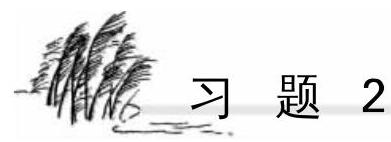
\includegraphics[max width=\textwidth, center]{2024_10_30_1bf34f7aeb61f11d11d3g-040}

1 若函数 $y=\frac{1}{2}\left(x^{2}-100 x+196+\left|x^{2}-100 x+196\right|\right)$ ,则当自变量 $x$ 取 1 , $2,3, \cdots, 100$ 这 100 个自然数时,函数值的和是()。\\
A. 540\\
B. 390\\
C. 194\\
D. 97\\
$2 \mathrm{Rt} \triangle A B C$ 的三个顶点 $A 、 B 、 C$ 均在抛物线 $y=x^{2}$ 上, 并且斜边 $A B$ 平行于 $x$ 轴。若斜边上的高为 $h$ ,则 ( )。\\
A. $h<1$\\
B. $h=1$\\
C. $1<h<2$\\
D. $h>2$

3 已知二次函数 $y=a x^{2}+b x+c$ 的系数 $a 、 b 、 c$ 都是整数,且 $f(19)=$ $f(99)=2005,|c|<1000$ ,则 $c$ 的值为多少?\\
4 二次函数 $y=a x^{2}+b x+c$ 的图象一部分如图所示,求 $a$ 的取值范围。\\
5 抛物线 $y=a x^{2}+b x+c$ 与 $x$ 轴交于 $A 、 B$ 两点,与 $y$ 轴交于点 $C$ ,若 $\triangle A B C$ 是直角三角形,则 $a c$ 的值为多少?\\
6 已知函数 $y=x^{2}-|x|-12$ 的图象与 $x$ 轴交于相异两点 $A 、 B$, 另一抛物线 $y=a x^{2}+b x+c$过 $A 、 B$ ,顶点为 $P$ ,且 $\triangle A P B$ 是等腰直角三角\\
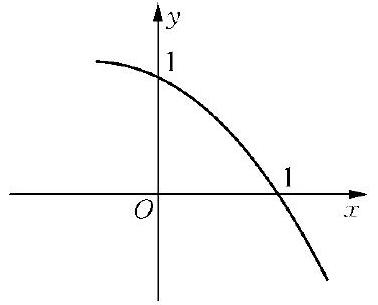
\includegraphics[max width=\textwidth, center]{2024_10_30_1bf34f7aeb61f11d11d3g-040(1)}\\
(第4题)

形,求 $a 、 b 、 c$ 。

7 已知二次函数 $y=a x^{2}+b x+c$ ,一次函数 $y=k(x-1)-\frac{k^{2}}{4}$ 。若它们的图象对于任意的实数 $k$ 都只有一个公共点, 求二次函数的解析式.\\
8 已知二次函数 $y=x^{2}+(a+1) x+b(a 、 b$ 为常数)。当 $x=3$ 时, $y=3$ ;当 $x$ 为任意实数时,都有 $y \geqslant x$ ,求抛物线的顶点到原点的距离。\\
9 已知实数 $a 、 b 、 c$ 满足 $(a+c)(a+b+c)<0$ 。求证:

\begin{align*}
(b-c)^{2}>4 a(a+b+c) .
\end{align*}

10 二次函数 $y=a x^{2}+b x+c(a \neq 0)$ 的图象经过点 $(-1,2)$ ,与 $x$ 轴交点的横坐标分别为 $x_{1} 、 x_{2}$, 其中 $-2 \leqslant x_{1}<-1,0<x_{2} \leqslant 1$, 求 $a$ 的取值范围。\\
11 已知二次函数 $y=a x^{2}(a \geqslant 1)$ 的图象上两点 $A 、 B$ 的横坐标分别为 -1 、 $2, O$ 是坐标原点. 如果 $\triangle A O B$ 是直角三角形,求 $\triangle O A B$ 的周长.\\
12 求抛物线族 $y=2 x^{2}-4 m x+2 m^{2}+m+1$ ( $m$ 为参数) 与 $\left(\frac{1}{8}, 1\right)$ 为圆心、 1 为半径的圆内部相交部分的面积。\\
13 设方程 $x^{2}-2 m x+m^{2}-1=0$ 的两个实根分别为 $\alpha 、 \beta . m$ 、 $k$ 满足什么关系时, $\alpha$ 、 $\beta$ 在方程 $x^{2}-2 m x+k=0$ 的两个实根之间?\\
14 设 $f(x)=a x^{2}+b x, a>0, a 、 b$ 都是整数。且当 $x=15$ 时, $y<0$ ;当 $x=16$ 时, $y>0$ 。\\
(1) 求证: $a \nmid b$ ,且 $b$ 是负整数;\\
(2)在 $x$ 取整数 $n$ 所得的所有函数值 $f(n)$ 中, 使 $f(n)$ 取最小值的 $n$ 是多少?\\
15 试求实数 $a 、 b$ ,使得函数 $y_{1}=x^{2}+a x+b$ 及 $y_{2}=x^{2}+b x+a$ 与 $x$ 轴的四个交点中相邻两点的距离都相等。

函数与一元二次方程

\section*{-、求一元二次方程的解}
方程 $a x^{2}+b x+c=0(a \neq 0)$ 称为一元二次方程, 一元二次方程是中学代数的重要内容之一,它与函数、不等式有密切的联系。

求一元二次方程解的主要方法有:配方法、公式法和因式分解法。\\
其中配方法是解一元二次方程的基本方法。而公式法是由配方法演绎的,可以得到一元二次方程的求根公式

\begin{align*}
x_{1,2}=\frac{-b \pm \sqrt{b^{2}-4 a c}}{2 a}\left(b^{2}-4 a c \geqslant 0\right) .
\end{align*}

有时也用因式分解法解一元二次方程,也就是如果一元二次方程的两根为 $x_{1} 、 x_{2}$ ,那么就有基本等式

\begin{align*}
\begin{aligned}
& a x^{2}+b x+c \\
= & a\left(x-x_{1}\right)\left(x-x_{2}\right)(a \neq 0),
\end{aligned}
\end{align*}

这是一个非常有用的等式。

\section*{二、根的判别式}
我们把 $\Delta=b^{2}-4 a c$ 叫做一元二次方程 $a x^{2}+b x+c=0(a \neq 0)$ 根的判别式. 根的判别式有以下的性质:\\
(1)方程有两个不相等的实数根 $\Longleftrightarrow \Delta>0$;\\
(2)方程有两个相等的实数根 $\Longleftrightarrow \Delta=0$;\\
(3)方程没有实数根 $\Longleftrightarrow \Delta<0$ 。\\
由此可知, $\Delta$ 的正负性关联着一元二次方程有无实根。

\section*{三、韦达定理}
若一元二次方程 $a x^{2}+b x+c=0(a \neq 0)$ 有两个根 $x_{1} 、 x_{2}$, 则 $x_{1} 、 x_{2}$ 与

方程的系数 $a 、 b 、 c$ 之间有以下关系:

\begin{align*}
\left\{\begin{array}{l}
x_{1}+x_{2}=-\frac{b}{a},  \tag{1}\\
x_{1} \cdot x_{2}=\frac{c}{a} .
\end{array}\right.
\end{align*}

这是法国数学家韦达(1540~1603 年)发现的定理。\\
如果给定一元二次方程 $a x^{2}+b x+c=0(a \neq 0)$ ,那么(1)与(2)式成立;反过来,如果两个数的和为 $m$ ,积为 $n$ ,那么这两个数是方程 $x^{2}-m x+n=0$ 的两个根。利用这一基本知识常可以简捷地处理问题。

更一般地,如果一元 $n$ 次方程\\
$a_{n} x^{n}+a_{n-1} x^{n-1}+\cdots+a_{1} x+a_{0}=0\left(a_{n} \neq 0\right)$ 的根为 $x_{1}, x_{2}, \cdots, x_{n}$ ,那么有

\begin{align*}
\left\{\begin{array}{l}
x_{1}+x_{2}+\cdots+x_{n}=-\frac{a_{n-1}}{a_{n}}, \\
x_{1} x_{2}+x_{1} x_{3}+\cdots+x_{n-1} x_{n}=\frac{a_{n-2}}{a_{n}}, \\
x_{1} x_{2} x_{3}+x_{1} x_{2} x_{4}+\cdots+x_{n-2} x_{n-1} x_{n}=-\frac{a_{n-3}}{a_{n}}, \\
\cdots \\
x_{1} x_{2} \cdots x_{n}=(-1)^{n} \frac{a_{0}}{a_{n}} .
\end{array}\right.
\end{align*}

例1 解方程 $x^{2}-|2 x-1|-4=0$ 。\\
分析 这是含绝对值符号的方程,需要找出 $2 x-1$ 的零点,再加以讨论。\\
解 当 $x \geqslant \frac{1}{2}$ 时,原方程化为

\begin{align*}
x^{2}-(2 x-1)-4=0,
\end{align*}

整理得

\begin{align*}
x^{2}-2 x-3=0,
\end{align*}

解得

\begin{align*}
x_{1}=3, x_{2}=-1 \text { (舍去). }
\end{align*}

当 $x<\frac{1}{2}$ 时, 原方程化为

\begin{align*}
x^{2}+(2 x-1)-4=0,
\end{align*}

整理得

\begin{align*}
x^{2}+2 x-5=0,
\end{align*}

解得

\begin{align*}
x_{3}=-1-\sqrt{6}, x_{4}=-1+\sqrt{6}(\text { 舍去 }) .
\end{align*}

所以原方程的解为 $x_{1}=3, x_{2}=-1-\sqrt{6}$.\\
例2 若 $a^{2}-3 a+1=0$ ,求 $3 a^{3}-8 a^{2}+a+\frac{3}{a^{2}+1}$ 的值。(重庆初三数学竞赛)

解 因为

\begin{align*}
a^{2}-3 a+1=0,
\end{align*}

即

\begin{align*}
a^{2}=3 a-1
\end{align*}

于是

\begin{align*}
\begin{aligned}
& 3 a^{3}-8 a^{2}+a+\frac{3}{a^{2}+1} \\
= & 3 a(3 a-1)-8(3 a-1)+a+\frac{1}{a} \\
= & 9 a^{2}-26 a+8+\frac{1}{a} \\
= & 9(3 a-1)-26 a+8+\frac{1}{a} \\
= & a+\frac{1}{a}-1
\end{aligned}
\end{align*}

又

\begin{align*}
a^{2}+1=3 a
\end{align*}

则

\begin{align*}
a+\frac{1}{a}=3
\end{align*}

故原式等于 2 。\\
评注 此题若用求根公式把 $a$ 算出,再代入所求的式子,则比较繁琑。处理这种类型的题目,可以通过对所求式子的"降次",从而起到简化运算的作用。

例3 解关于 $x$ 的方程 $(m-1) x^{2}+(2 m-1) x+m-3=0$.\\
解 对 $m$ 讨论。\\
(1)当 $m=1$ ,原方程为

\begin{align*}
\begin{gathered}
x-2=0 \\
x=2
\end{gathered}
\end{align*}

(2)当 $m \neq 1$ ,原方程为一元二次方程,可得

\begin{align*}
\begin{aligned}
\Delta & =(2 m-1)^{2}-4(m-1)(m-3) \\
& =12 m-11
\end{aligned}
\end{align*}

当 $m<\frac{11}{12}$ 时, $\Delta<0$, 方程无实数根;

当 $m=\frac{11}{12}$ 时, $\Delta=0$ ,方程有两个相等的实数根

\begin{align*}
x_{1,2}=\frac{1-2 m}{2(m-1)}=5
\end{align*}

当 $m>\frac{11}{12}$ 时, $\Delta>0$, 方程有两个不相等的实数根

\begin{align*}
x_{1,2}=\frac{(1-2 m) \pm \sqrt{12 m-11}}{2(m-1)}
\end{align*}

例 4 若方程 $\left(x^{2}-1\right)\left(x^{2}-4\right)=k$ 有 4 个非零实数根,且它们在数轴上对应的 4 个点等距排列, 求 $k$ 的值. (全国初中数学竞赛题)

解法一 令 $x^{2}=t$, 则原方程为

\begin{align*}
\begin{aligned}
& (t-1)(t-4)=k \\
& t^{2}-5 t+4-k=0
\end{aligned}
\end{align*}

整理得\\
则由求根公式和题意得

\begin{align*}
t_{1,2}=\frac{5 \pm \sqrt{9+4 k}}{2}>0
\end{align*}

所以 4 个非零实数根分别为

\begin{align*}
\begin{aligned}
& x_{1}=-\sqrt{\frac{5+\sqrt{9+4 k}}{2}}, x_{2}=-\sqrt{\frac{5-\sqrt{9+4 k}}{2}}, \\
& x_{3}=\sqrt{\frac{5-\sqrt{9+4 k}}{2}}, x_{4}=\sqrt{\frac{5+\sqrt{9+4 k}}{2}} .
\end{aligned}
\end{align*}

由题意它们在数轴上对应的点等距排列,所以得到

\begin{align*}
\begin{gathered}
3 \sqrt{\frac{5-\sqrt{9+4 k}}{2}}=\sqrt{\frac{5+\sqrt{9+4 k}}{2}} \\
k=\frac{7}{4}
\end{gathered}
\end{align*}

化简得\\
解法二 由题意, 4 个非零实数根在数轴上对应的 4 个等距点中有两对关于原点对称,则可令

\begin{align*}
\begin{aligned}
& \left(x^{2}-1\right)\left(x^{2}-4\right)-k \\
= & (x+3 a)(x+a)(x-a)(x-3 a),
\end{aligned}
\end{align*}

即

\begin{align*}
x^{4}-5 x^{2}+4-k=x^{4}-10 a^{2} x^{2}+9 a^{4},
\end{align*}

\section*{于是有}
\begin{align*}
\begin{aligned}
& \left\{\begin{array}{l}
10 a^{2}=5, \\
9 a^{4}=4-k,
\end{array}\right. \\
& k=\frac{7}{4} .
\end{aligned}
\end{align*}

解得\\
例5 在直角坐标系中,抛物线 $y=x^{2}+m x-\frac{3}{4} m^{2}(m>0)$ 与 $x$ 轴交于 $A 、 B$ 两点, 若 $A 、 B$ 两点到原点的距离分别为 $O A 、 O B$, 且满足 $\frac{1}{O B}-\frac{1}{O A}=$ $\frac{2}{3}$ ,求 $m$ 的值。

分析 根据 $m$ 为正数的条件,先判断 $A 、 B$ 两点的位置,从而把距离 $O A$ 、 $O B$ 用其坐标表示。

解 设方程 $x^{2}+m x-\frac{3}{4} m^{2}=0$ 的两个根分别为 $x_{1} 、 x_{2}$ ,且 $x_{1}<x_{2}$ ,则有

\begin{align*}
x_{1}+x_{2}=-m<0, x_{1} \cdot x_{2}=-\frac{3}{4} m^{2}<0
\end{align*}

所以 $x_{1}<0, x_{2}>0$, 由 $\frac{1}{O B}-\frac{1}{O A}=\frac{2}{3}$, 可知 $O A>O B$, 又 $m>0$, 所以抛物线的对称轴在 $y$ 轴的左侧,于是 $O A=\left|x_{1}\right|=-x_{1}, O B=x_{2}$ 。

则有

\begin{align*}
\begin{gathered}
\frac{1}{x_{1}}+\frac{1}{x_{2}}=\frac{2}{3} \\
\frac{x_{1}+x_{2}}{x_{1} x_{2}}=\frac{-m}{-\frac{3}{4} m^{2}}=\frac{2}{3}, \\
m=2 .
\end{gathered}
\end{align*}

即

解得\\
例 6 已知方程 $x^{2}+(2 k-1) x-k+1=0$ 。\\
(1)当 $k$ 为何值时,方程有一根为正、一根为负?\\
(2)当 $k$ 为何值时,方程两根都为正数?\\
(3)当 $k$ 为何值时,方程一根大于 1 、一根小于 1 ?\\
解 设方程的两根为 $x_{1}, x_{2}$ 。\\
(1)由题意得

\begin{align*}
\left\{\begin{array}{l}
\Delta=(2 k-1)^{2}-4 \times(-k+1)>0 \\
x_{1} \cdot x_{2}=-k+1<0
\end{array}\right.
\end{align*}

\begin{align*}
k>1
\end{align*}

(2)由题意得

\begin{align*}
\left\{\begin{array}{l}
\Delta=4 k^{2}-3 \geqslant 0 \\
x_{1}+x_{2}=1-2 k>0 \\
x_{1} \cdot x_{2}=-k+1>0
\end{array}\right.
\end{align*}

解得

\begin{align*}
k \leqslant-\frac{\sqrt{3}}{2}
\end{align*}

(3)由题意得

\begin{align*}
\left(x_{1}-1\right)\left(x_{2}-1\right)<0,
\end{align*}

即

\begin{align*}
x_{1} x_{2}-\left(x_{1}+x_{2}\right)+1<0,
\end{align*}

由韦达定理得

\begin{align*}
(-k+1)-(1-2 k)+1<0,
\end{align*}

所以

\begin{align*}
k<-1
\end{align*}

评注 实际上,在处理"方程的两个根为一正一负"这样的题目时,可以直接由 $x_{1} \cdot x_{2}=\frac{c}{a}<0$ 来解,不需要 $\Delta>0$ 。在处理"两根中一根比某数 $a$ 大,一根比 $a$ 小"的情况时,可用 $\left(x_{1}-a\right)\left(x_{2}-a\right)<0$ 来解决。若要求"方程的两根都大于某数 $a$ ",则可用 $\Delta \geqslant 0,\left(x_{1}-a\right)+\left(x_{2}-a\right)>0,\left(x_{1}-a\right) \cdot\left(x_{2}-\right.$ a) $>0$ 这 3 个不等式来解决。注意千万不要用 $\Delta \geqslant 0, x_{1} \cdot x_{2} \geqslant a^{2}, x_{1}+x_{2} \geqslant$ $2 a$ ,这样是错误的。

例7 求方程 $x+y=x^{2}-x y+y^{2}+1$ 的实数解。\\
解 将原方程看作关于 $x$ 的一元二次方程

\begin{align*}
x^{2}-(y+1) x+y^{2}-y+1=0 .
\end{align*}

要使此方程有实数解,则

\begin{align*}
\begin{aligned}
\Delta & =(y+1)^{2}-4\left(y^{2}-y+1\right) \\
& =-3 y^{2}+6 y-3 \\
& =-3(y-1)^{2} \\
& \geqslant 0
\end{aligned}
\end{align*}

因为

\begin{align*}
-3(y-1)^{2} \leqslant 0
\end{align*}

所以

\begin{align*}
\left\{\begin{array}{l}
y=1, \\
x=1 .
\end{array}\right.
\end{align*}

评注 在求解二元二次(或含字母)方程时,其基本思路之一,就是根据

方程有实数解,运用判别式分离变元然后逐一讨论,求得结果。\\
例 8 设 $a 、 b$ 是方程 $x^{2}+68 x+1=0$ 的两个根, $c, d$ 是方程 $x^{2}-86 x+$ $1=0$ 的两个根,求 $(a+c)(b+c)(a-d)(b-d)$ 的值。

分析 题目中有 4 个字母 $a 、 b 、 c 、 d$ ,则根据韦达定理,先转化为 2 个字母的式子,再利用条件来解决。

解 根据韦达定理有 $a b=c d=1, a+b=-68$ ,则\\
$(a+c)(b+c)(a-d)(b-d)=\left[a b+(a+b) c+c^{2}\right] \cdot\left[a b-(a+b) d+d^{2}\right]$,代入得 $(a+c)(b+c)(a-d)(b-d)=\left(1-68 c+c^{2}\right) \cdot\left(1+68 d+d^{2}\right)$.

又因为 $c 、 d$ 是方程 $x^{2}-86 x+1=0$ 的两个根, 则

\begin{align*}
c^{2}-86 c+1=0 \Rightarrow c^{2}-68 c+1=18 c .
\end{align*}

同理 $d^{2}+68 d+1=154 d$ ,所以 $(a+c)(b+c)(a-d)(b-d)=18 c \cdot$ $154 d=2772$.

例 9 在满足 $(x-3)^{2}+(y-3)^{2}=6$ 的所有实数对 $(x, y)$ 中, 求 $\frac{y}{x}$ 的最大值.

分析 粗看此题似乎无法解,符合条件的实数对 $(x, y)$ 有无数对,相应的 $\frac{y}{x}$ 值无法一一求出比较. 为了解决这个题目, 我们这里可以引进比值 $t=$ $\frac{y}{x}$ ,将原式转化为关于 $x$ 的二次方程。

解 设 $t=\frac{y}{x}$, 则 $y=t x$, 代入已知等式, 整理为关于 $x$ 的二次方程

\begin{align*}
\left(1+t^{2}\right) x^{2}-6(1+t) x+12=0
\end{align*}

因为此方程有实数解, 则

\begin{align*}
\Delta=36(t+1)^{2}-4 \times 12 \times\left(t^{2}+1\right) \geqslant 0,
\end{align*}

整理为

\begin{align*}
t^{2}-6 t+1 \leqslant 0
\end{align*}

解得

\begin{align*}
3-2 \sqrt{2} \leqslant t \leqslant 3+2 \sqrt{2}
\end{align*}

所以 $\frac{y}{x}$ 的最大值为 $3+2 \sqrt{2}$.\\
评注 例 9 通过构造一个二次方程,创造出利用根的判别式 $\Delta \geqslant 0$ 的条件,从而求得最值,这在求一些最值的题目中经常用到。

例10 设方程 $\left|x^{2}+a x\right|=4$ 只有三个不相等的实数根,求 $a$ 的值和相应的 3 个根。(重庆初中数学竞赛)

同理 $\Delta_{2}$ 和 $\Delta_{4}$ 中也必有一个大于零, 故 $\Delta_{1} 、 \Delta_{2} 、 \Delta_{3} 、 \Delta_{4}$ 中至少有两个大于零,即所得的四个方程中至少有两个方程有两个不相等的实数根。

评注 因本题中的 $a 、 b 、 c 、 d$ 是轮换对称的, 故单独去判断四个方程的判别式是否大于零, 则较困难. 所以本题的关键是判断 $\Delta_{1}+\Delta_{3}$ 和 $\Delta_{2}+\Delta_{4}$ 是大于零的,从而起到柳暗花明又一村的效果。

例12 已知方程 $x^{2}+a_{1} x+a_{2} a_{3}=0$ 与方程 $x^{2}+a_{2} x+a_{1} a_{3}=0$ 有且只有一个非零公共根,求证:这两个方程的另两个根(除去公共根外)是方程 $x^{2}+$ $a_{3} x+a_{1} a_{2}=0$ 的两个根. (山东省初中数学竞赛)

证明 设 $\alpha 、 \beta$ 是方程 $x^{2}+a_{1} x+a_{2} a_{3}=0$ 的两个根, $\alpha, \gamma$ 是方程 $x^{2}+a_{2} x+$ $a_{1} a_{3}=0$ 的两个根,则得到

两式相减得

\begin{align*}
\alpha\left(a_{1}-a_{2}\right)+a_{3}\left(a_{2}-a_{1}\right)=0,
\end{align*}

因为

\begin{align*}
a_{1} \neq a_{2},
\end{align*}

所以\\
又因为

\begin{align*}
\alpha \cdot \beta=a_{2} \cdot a_{3}
\end{align*}

\begin{align*}
\alpha \cdot \gamma=a_{1} \cdot a_{3},
\end{align*}

则

\begin{align*}
\beta=a_{2}, \gamma=a_{1} .
\end{align*}

把 $\alpha=a_{3}$ 代入方程

\begin{align*}
x^{2}+a_{1} x+a_{2} a_{3}=0,
\end{align*}

因为 $a_{3} \neq 0$, 则

\begin{align*}
a_{1}+a_{2}+a_{3}=0,
\end{align*}

所以得到

\begin{align*}
\left\{\begin{array}{l}
\beta+\gamma=a_{2}+a_{1}=-a_{3}, \\
\beta \cdot \gamma=a_{2} a_{1},
\end{array}\right.
\end{align*}

由韦达定理可知, $\beta 、 \gamma$ 是方程 $x^{2}+a_{3} x+a_{1} a_{2}=0$ 的两个根。\\
例13 已知方程 $x^{2}+p x+q=0$ 的两根为 1997 和 1998,当 $x$ 依次取整数 $0,1,2, \cdots, 1999$ 时,二次三项式 $y=x^{2}+p x+q$ 的对应值依次为 $y_{0}, y_{1}$ , $y_{2}, \cdots, y_{1999}$ 。求这些值中能被 6 整除的个数。

解 因为方程的 $x^{2}+p x+q=0$ 的两根为 1997 和 1998 , 则

\begin{align*}
y=(x-1997)(x-1998),
\end{align*}

由此式可知,当 $x$ 取整数时,所有 $y$ 值都能被 2 整除。\\
要使二次三项式对应的值能被 6 整除,只需考察两因式能被 3 整除的情况即可。\\
(1)当 $x-1997=3 k$ 时,则

\begin{align*}
x-1998=3 k-1,
\end{align*}

因为

\begin{align*}
0 \leqslant x \leqslant 1999
\end{align*}

所以

\begin{align*}
-1997 \leqslant 3 k \leqslant 2
\end{align*}

此时, $k$ 可取从一665到 0 共 666 个值。\\
(2)当 $x-1998=3 k$ 时,则

\begin{align*}
x-1997=3 k+1,
\end{align*}

因为

\begin{align*}
0 \leqslant x \leqslant 1999
\end{align*}

所以

\begin{align*}
-1998 \leqslant 3 k \leqslant 1
\end{align*}

此时, $k$ 可取从一666到 0 共 667 个值.\\
综上可得,所有取值中能被 6 整除的值的个数共为

\begin{align*}
667+666=1333
\end{align*}

例14 已知二次函数 $f(x)=x^{2}+p x+q$, 并且方程 $f(x)=0$ 与 $f(2 x)=$ 0 有相同的非零实根。\\
(1) 求 $\frac{q}{p^{2}}$ 的值;\\
(2)若 $f(1)=28$ ,解方程 $f(x)=0$ 。(四川省初中数学竞赛)\\
解 (1) 设 $f(x)=0$ 的两个根为 $x_{1} 、 x_{2}$, 且 $x_{1} \leqslant x_{2}$, 则

\begin{align*}
\begin{aligned}
f(x) & =\left(x-x_{1}\right)\left(x-x_{2}\right), \\
f(2 x) & =\left(2 x-x_{1}\right)\left(2 x-x_{2}\right) \\
& =4\left(x-\frac{x_{1}}{2}\right)\left(x-\frac{x_{2}}{2}\right)
\end{aligned}
\end{align*}

由此可知 $f(2 x)=0$ 的两根为 $\frac{x_{1}}{2} 、 \frac{x_{2}}{2}$, 且 $\frac{x_{1}}{2} \leqslant \frac{x_{2}}{2}$.\\
由题意 $f(x)=0$ 和 $f(2 x)=0$ 有相同的非零实根, 所以得

\begin{align*}
x_{1}=\frac{x_{2}}{2}
\end{align*}

故

\begin{align*}
\frac{q}{p^{2}}=\frac{x_{1} \cdot x_{2}}{\left(x_{1}+x_{2}\right)^{2}}=\frac{x_{1} \cdot 2 x_{1}}{\left(x_{1}+2 x_{1}\right)^{2}}=\frac{2}{9} .
\end{align*}

(2) 因为 $f(1)=28$, 则

\begin{align*}
\left(1-x_{1}\right)\left(1-x_{2}\right)=28,
\end{align*}

又由第(1)小题得

\begin{align*}
\left(1-x_{1}\right)\left(1-2 x_{1}\right)=28
\end{align*}

解得

\begin{align*}
x_{1}=-3 \text { 或 } \frac{9}{2} \text {, }
\end{align*}

进而

\begin{align*}
x_{2}=-6 \text { 或 } 9,
\end{align*}

故 $f(x)=0$ 的两组解为

\begin{align*}
\left\{\begin{array} { l } 
{ x _ { 1 } = - 3 , } \\
{ x _ { 2 } = - 6 , }
\end{array} \text { 或 } \left\{\begin{array}{l}
x_{1}=\frac{9}{2}, \\
x_{2}=9 .
\end{array}\right.\right.
\end{align*}

例 15 已知关于 $x$ 的一元二次方程 $x^{2}+c x+a=0$ 的两个整数根恰好比方程 $x^{2}+a x+b=0$ 的两个根都大 1 ,求 $a+b+c$ 的值。

解 设方程 $x^{2}+a x+b=0$ 的两个根为 $\alpha, \beta$, 其中 $\alpha, \beta$ 为整数, 且 $\alpha \leqslant \beta$,则方程 $x^{2}+c x+a=0$ 的两根为 $\alpha+1 、 \beta+1$, 则易知 $a, b, c$ 都为整数, 由题意得

\begin{align*}
\alpha+\beta=-a,(\alpha+1)(\beta+1)=a,
\end{align*}

两式相加得

\begin{align*}
\alpha \beta+2 \alpha+2 \beta+1=0,
\end{align*}

即

\begin{align*}
(\alpha+2)(\beta+2)=3,
\end{align*}

所以

\begin{align*}
\left\{\begin{array} { l } 
{ \alpha + 2 = 1 , } \\
{ \beta + 2 = 3 , }
\end{array} \text { 或 } \left\{\begin{array}{l}
\alpha+2=-3, \\
\beta+2=-1,
\end{array}\right.\right.
\end{align*}

解得

\begin{align*}
\left\{\begin{array} { l } 
{ \alpha = - 1 , } \\
{ \beta = 1 , }
\end{array} \text { 或 } \left\{\begin{array}{l}
\alpha=-5, \\
\beta=-3 .
\end{array}\right.\right.
\end{align*}

又因为 $a=-(\alpha+\beta), b=\alpha \beta, c=-[(\alpha+1)+(\beta+1)]$,\\
所以

\begin{align*}
a=0, b=-1, c=-2 \text { 或者 } a=8, b=15, c=6 \text {, }
\end{align*}

故

\begin{align*}
a+b+c=-3 \text { 或 } 29 \text {. }
\end{align*}

\begin{center}
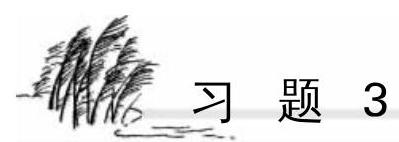
\includegraphics[max width=\textwidth]{2024_10_30_1bf34f7aeb61f11d11d3g-054}
\end{center}

1 若实数 $a 、 b$ 满足 $\frac{1}{2} a-a b+b^{2}+2=0$ ,则 $a$ 的取值范围是()。\\
A. $a \leqslant-2$\\
B. $a \geqslant 4$\\
C. $a \leqslant-2$ 或 $a \geqslant 4$\\
D. $-2 \leqslant a \leqslant 4$

2 已知实数 $a \neq b$, 且满足 $(a+1)^{2}=3-3(a+1), 3(b+1)=3-(b+1)^{2}$.则 $b \sqrt{\frac{b}{a}}+a \sqrt{\frac{a}{b}}$ 的值为 ( )。\\
A. 23\\
B. -23\\
C. -2\\
D. -13

3 形如 $x^{2}+b x-c=0$ 或形如 $x^{2}-b x-c=0$ 的方程,其中的 $b 、 c$ 为 1,2 , $3 , \cdots , 9$ 中的一个正整数,且方程至少有一根也为 $1,2, \cdots, 9$ 中的一个正整数,就称该方程为"漂亮方程"。则"漂亮方程"的个数为()。\\
A. 20\\
B. 22\\
C. 24\\
D. 26

4 已知方程 $x^{2}-5 x-2=0$ 的一个根为 $a$ ,那么 $a+\frac{2}{a}$ 的值是多少?\\
5 若 $a 、 b$ 为实数,求证关于 $x$ 的一元二次方程 $(x-a)(x-a-b)=1$ 的两根中的一根大于 $a$ ,另一根小于 $a$ 。\\
6 已知关于 $x$ 的二次方程 $x^{2}-a x+a^{2}-4=0$ 。\\
(1) $a$ 为何值时,方程有两个不同正根?\\
(2) $a$ 为何值时,方程只有一个正根?\\
(3) $a$ 为何值时,方程有一正根、一负根?\\
7 求方程 $x^{2}+3 x-\frac{3}{x^{2}+3 x-7}=9$ 的全体实数根的乘积。\\
8 若自然数 $a 、 b$ 满足 $a^{2}+b^{2}-2 a-4 b+4<0$ ,设方程 $a x^{2}+b x-3=0$ 的正根为 $p$ ,方程 $a x^{2}-b x-399=0$ 的负根为 $q$ ,求 $p q$ 的值。\\
9 已知关于 $x$ 的三个方程:(1) $x^{2}-x+m=0$ ,(2) $(m-1) x^{2}+2 x+1=0$ , (3) $(m-2) x^{2}+2 x-1=0$ 。若其中至少有两个方程有实数根, 求实数 $m$ 的取值范围。\\
10 如果方程 $(x-1)\left(x^{2}-2 x+m\right)=0$ 的三根可作为一个三角形的三边之长,求实数 $m$ 的取值范围。\\
11 已知一元二次方程 $x^{2}-x+1-m=0$ 的两根为 $x_{1} 、 x_{2}$ ,满足 $\left|x_{1}\right|+$ $\left|x_{2}\right| \leqslant 5$ ,求实数 $m$ 的取值范围。

12 已知实数 $x 、 y$ 满足 $x^{2}+4 y^{2} \leqslant 1$, 求 $\frac{1}{4} x^{2}+y^{2}+3 x y$ 的最大值.\\
13 已知方程 $x^{2}+b x+c=0$ 及 $x^{2}+c x+b=0$ 分别有两个整数根 $x_{1} 、 x_{2}$ 和 $x_{1}^{\prime} 、 x_{2}^{\prime}$ ,且 $x_{1} x_{2}>0, x_{1}^{\prime} x_{2}^{\prime}>0$ 。求证: $b-1 \leqslant c \leqslant b+1$ 。\\
14 若 $a 、 b 、 c$ 均为实数,且 $a+b+c=0, a b c=2$ ,那么 $|a|+|b|+|c|$ 的最小值可达到多少?\\
15 已知关于 $x$ 的方程

\begin{align*}
\frac{(a+1)(b+1)}{x+2}+\frac{(a-1)(b-1)}{x-2}=\frac{2 a b}{x}
\end{align*}

无解,实数 $a 、 b$ 满足 $(a-b) a b \neq 0$ 。求 $\frac{a}{b}+\frac{b}{a}$ 的值.

一元二次不等式经过化简后,一般可以表示成下面的两种形式之一:\\
(1) $a x^{2}+b x+c>0(a>0)$;\\
(2) $a x^{2}+b x+c<0(a>0)$.

若 $\Delta=b^{2}-4 a c<0$ ,不等式(1)的解为全体实数,不等式(2)为无解。\\
若 $\Delta=b^{2}-4 a c=0$ ,不等式(1)的解为 $x \neq-\frac{b}{2 a}$ 的实数,不等式(2)的解为无解。

若 $\Delta=b^{2}-4 a c>0$ ,我们可以先考查与之对应的一元二次方程的两根 $x_{1} 、 x_{2}$ ,此时不等式(1)的解的情况是:"两头跑"(小于小根,大于大根),不等式(2)的解的情况是:"中间找"(大于小根,小于大根)。

二次函数、二次方程及二次不等式三者之间有着密切的联系,求解一元二次不等式时,注意利用二次函数的图象以及对应的一元二次方程的判别式。

例1 解关于 $x$ 的不等式

\begin{align*}
2 x+\sqrt{x}>3
\end{align*}

解 原不等式可化为

\begin{align*}
2(\sqrt{x})^{2}+\sqrt{x}-3>0
\end{align*}

即

\begin{align*}
(2 \sqrt{x}+3)(\sqrt{x}-1)>0
\end{align*}

因为

\begin{align*}
2 \sqrt{x}+3>0
\end{align*}

则

\begin{align*}
\sqrt{x}-1>0
\end{align*}

所以

\begin{align*}
\sqrt{x}>1
\end{align*}

解得

\begin{align*}
x>1
\end{align*}

例2 解关于 $x$ 的不等式

\begin{align*}
5|x|+24<x^{2}
\end{align*}

解法一 当 $x \geqslant 0$ 时, 原不等式可化为

\begin{align*}
x^{2}-5 x-24>0,
\end{align*}

即

\begin{align*}
(x-8)(x+3)>0,
\end{align*}

解得

\begin{align*}
x>8 .
\end{align*}

当 $x<0$ 时,原不等式可化为

即

\begin{align*}
x^{2}+5 x-24>0,
\end{align*}

解得

\begin{align*}
(x+8)(x-3)>0,
\end{align*}

\begin{align*}
x<-8
\end{align*}

所以,原不等式解为

\begin{align*}
x>8 \text { 或 } x<-8 .
\end{align*}

解法二 因为 $x^{2}=|x|^{2}$ ,则原不等式可化为

\begin{align*}
|x|^{2}-5|x|-24>0,
\end{align*}

即

\begin{align*}
(|x|-8)(|x|+3)>0,
\end{align*}

因为

\begin{align*}
|x|+3>0
\end{align*}

则解为

\begin{align*}
|x|>8
\end{align*}

所以,不等式解为

\begin{align*}
x>8 \text { 或 } x<-8 .
\end{align*}

说明 本题也可以利用函数 $y=x^{2}-5|x|-24$ 的图象来解。先作函数 $y=x^{2}-5 x-24$ 的图象,再保持 $y$ 轴右边的图象不变,然后把这部分图象关于 $y$ 轴对称地翻到左边,得到的关于 $y$ 轴成对称的曲线就是函数 $y=x^{2}-5|x|-$ 24 的图象。

例 3 若不等式 $\frac{1}{p} x^{2}+q x+p>0$ 的解为 $2<x<4$, 求实数 $p 、 q$ 的值.\\
解 由题意知 $p<0$ 且 2、4 是方程 $\frac{1}{p} x^{2}+q x+p=0$ 的两个根,则有

\begin{align*}
\left\{\begin{array}{l}
2+4=-p q, \\
2 \cdot 4=p^{2}, \\
p<0,
\end{array}\right.
\end{align*}

解得

\begin{align*}
\left\{\begin{array}{l}
p=-2 \sqrt{2}, \\
q=\frac{3 \sqrt{2}}{2} .
\end{array}\right.
\end{align*}

例 4 设 $a$ 为参数,解关于 $x$ 的一元二次不等式 $a x^{2}-(a+1) x+1<0$ 。\\
解 (1)当 $a=0$ 时,原不等式化为

\begin{align*}
\begin{gathered}
-x+1<0 \\
x>1
\end{gathered}
\end{align*}

(2)当 $a \neq 0$ 时,原不等式可化为

\begin{align*}
a\left(x-\frac{1}{a}\right)(x-1)<0 .
\end{align*}

(i)若 $a>0$ ,则化为

\begin{align*}
\left(x-\frac{1}{a}\right)(x-1)<0 .
\end{align*}

当 $\frac{1}{a}>1$ 时, 即 $0<a<1$, 解为

\begin{align*}
1<x<\frac{1}{a}
\end{align*}

当 $\frac{1}{a}<1$ 时, 即 $a>1$ 时, 解为

\begin{align*}
\frac{1}{a}<x<1
\end{align*}

当 $\frac{1}{a}=1$ 时,即 $a=1$ 时,不等式无解。\\
(ii)若 $a<0$ ,则可化为

\begin{align*}
\begin{gathered}
\left(x-\frac{1}{a}\right)(x-1)>0, \\
x>1 \text { 或 } x<\frac{1}{a} .
\end{gathered}
\end{align*}

解为\\
所以, $a=0$ 时不等式解为 $x>1 ; a>1$ 时,不等式解为 $\frac{1}{a}<x<1 ; 0<$ $a<1$ 时,不等式解为 $1<x<\frac{1}{a} ; a=1$ 时,不等式无解; $a<0$ 时,不等式解

为 $x>1$ 或 $x<\frac{1}{a}$.\\
评注 本例对 $a$ 的讨论分三层:\\
(1)讨论 $a$ 是否为 0 ;\\
(2)讨论 $a$ 的正负性,这是由于在进一步的变形中,不等式两边需除以 $a$ ,由不等式的性质知,除数的符号将影响不等号的方向;\\
(3)讨论 $\frac{1}{a}$ 与 1 的大小关系。\\
例 5 已知二次函数 $f(x)=a x^{2}+b x+c$ 的图象如图 4-1所示,

记 $p=|a-b+c|+|2 a+b|, q=\mid a+b+$ $c|+|2 a-b|$, 试比较 $p 、 q$ 的大小。

分析 要比较 $p 、 q$ 的大小,关键是利用二次函数的图象和性质把 $p 、 q$ 表达式的绝对值去掉。

解 由题意得

\begin{align*}
a<0, b>0, c=0,
\end{align*}

\begin{center}
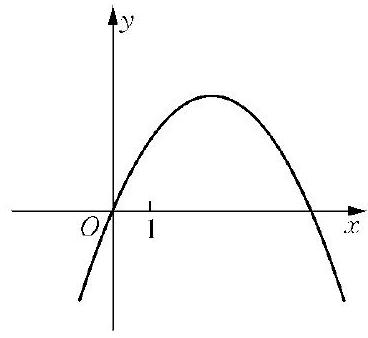
\includegraphics[max width=\textwidth]{2024_10_30_1bf34f7aeb61f11d11d3g-059}
\end{center}

图4-1

所以 $p=|a-b|+|2 a+b|, q=|a+b|+|2 a-b|$.\\
又 $-\frac{b}{2 a}>1$, 所以 $-b<2 a$, 则 $2 a+b>0$, 从而 $a+b>-a>0$, 则

\begin{align*}
\begin{aligned}
& p=|a-b|+|2 a+b|=b-a+2 a+b=2 b+a, \\
& q=|a+b|+|2 a-b|=a+b+b-2 a=2 b-a
\end{aligned}
\end{align*}

所以 $p<q$.\\
例 6 已知不等式 $\left(m^{2}+4 m-5\right) x^{2}-4(m-1) x+3>0$ 对一切实数 $x$恒成立,求实数 $m$ 的取值范围。

解(1)当 $m^{2}+4 m-5=0$ 时,得

\begin{align*}
m=1 \text { 或 } m=-5 \text {. }
\end{align*}

当 $m=1$ 时, 原不等式化为 $3>0$ ,恒成立;\\
当 $m=-5$ 时,原不等式化为 $24 x+3>0$ ,不恒成立。\\
(2)当 $m^{2}+4 m-5 \neq 0$ 时,由于原不等式对一切实数 $x$ 恒成立,则有

\begin{align*}
\left\{\begin{array}{l}
m^{2}+4 m-5>0 \\
\Delta=16(m-1)^{2}-4\left(m^{2}+4 m-5\right) \times 3<0
\end{array}\right.
\end{align*}

解得

\begin{align*}
\left\{\begin{array}{l}
m>1 \text { 或 } m<-5, \\
1<m<19,
\end{array}\right.
\end{align*}

则 $m$ 的范围为 $1<m<19$.

综合(1)、(2),当 $1 \leqslant m<19$ 时,原不等式恒成立。\\
评注 本题有很多种变型,例如不等式: $\frac{3 x^{2}+k x+2 k}{x^{2}+x+2}>2$ 对一切 $x$ 恒成立,求 $k$ 的取值范围。从形式上看,此题是分式不等式,但因为分母 $x^{2}+x+$ $2=\left(x+\frac{1}{2}\right)^{2}+\frac{7}{4}>0$ ,故原不等式可转化为一元二次不等式,然后类同于上例,解出 $k$ 的范围。

例7 若抛物线 $y=x^{2}+a x+2$ 与连结两点 $M(0,1) 、 N(2,3)$ 的线段 (包括 $M 、 N$ 两点)有两个相异的交点,求 $a$ 的取值范围。

解 设过两点 $M 、 N$ 的直线为 $y=k x+b$ ,则

\begin{align*}
\left\{\begin{array}{l}
1=0 \times k+b, \\
3=2 \times k+b,
\end{array}\right.
\end{align*}

解得

\begin{align*}
\left\{\begin{array}{l}
k=1 \\
b=1
\end{array}\right.
\end{align*}

所以

\begin{align*}
y=x+1
\end{align*}

要使抛物线 $y=x^{2}+a x+2$ 与线段 $M N$ 有两个相异的交点,等价于方程 $x^{2}+a x+2=x+1$ 在 $0 \leqslant x \leqslant 2$ 上有两个不同的根。令

\begin{align*}
f(x)=x^{2}+(a-1) x+1,
\end{align*}

由函数图象可知, $f(x)$ 的图象与 $x$ 轴的两个不同交点位于 0 与 2 之间,因满足在 $x=0$ 和 $x=2$ 处的函数值均大于或等于 0 ,对称轴也在 $x=0$ 与 $x=2$ 之间,即有

\begin{align*}
\left\{\begin{array}{l}
\Delta=(a-1)^{2}-4>0 \\
f(0)=1 \geqslant 0 \\
f(2)=4+2(a-1)+1 \geqslant 0 \\
0<-\frac{a-1}{2}<2 \\
\\
\quad-\frac{3}{2} \leqslant a<-1
\end{array}\right.
\end{align*}

解得

因此当 $-\frac{3}{2} \leqslant a<1$ 时,有两个相异的交点。\\
评注 本题可能有很多同学直接用 $\Delta \geqslant 0$, 解得 $a>3$ 或 $a<-1$, 这样做

法是错误的. 因为题目要求是抛物线与线段有两个不同交点,即等价于所令的二次函数 $f(x)$ 在 0 与 2 之间与 $x$ 轴有两个交点, 所以要再根据图象得到另外 3 个应满足的式子。

例 8 已知不等式 $a x^{2}+b x+c>0$ 的解是 $\alpha<x<\beta$ (其中 $\alpha>0$ ). 试求不等式 $c x^{2}-b x+a>0$ 的解。

解 由题意不等式 $a x^{2}+b x+c>0$ 的解是 $\alpha<x<\beta$, 则可得 $a<0$, 且

\begin{align*}
a x^{2}+b x+c=a(x-a)(x-\beta)
\end{align*}

由韦达定理得

\begin{align*}
\left\{\begin{array}{l}
\alpha+\beta=-\frac{b}{a}, \\
\alpha \cdot \beta=\frac{c}{a},
\end{array}\right.
\end{align*}

从而有

\begin{align*}
\begin{aligned}
& c x^{2}-b x+a \\
= & a \alpha \beta x^{2}+a(\alpha+\beta) x+a \\
= & a\left[\alpha \beta x^{2}+(\alpha+\beta) x+1\right] \\
= & a(\alpha x+1)(\beta x+1) .
\end{aligned}
\end{align*}

又因为

\begin{align*}
a<0, \beta>\alpha>0,
\end{align*}

则得到

\begin{align*}
0>-\frac{1}{\beta}>-\frac{1}{\alpha},
\end{align*}

所以所求不等式的解为

\begin{align*}
-\frac{1}{\alpha}<x<-\frac{1}{\beta} .
\end{align*}

说明 实际上, 如果一元二次方程 $a x^{2}+b x+c=0$ 的两根为 $\alpha, \beta$, 那么方程 $c x^{2}-b x+a=0$ 的两根为 $\alpha 、 \beta$ 的倒数的相反数 $-\frac{1}{\alpha} 、-\frac{1}{\beta}$ 。

例 9 已知三角形三条边 $a 、 b 、 c$ 满足

\begin{align*}
\begin{gathered}
a^{2}+2 b-12 c+15=0 \\
a+2 b-6 c+9=0
\end{gathered}
\end{align*}

若最大边 $a$ 是整数,求 $a 、 b 、 c$.\\
分析 可以把 $a$ 看作常数, 由两个方程解出 $b$ 和 $c$, 再根据三角形的性质和 $a$ 为最大边且 $a$ 是整数的条件, 求得 $a 、 b 、 c$ 。

\section*{解 由已知两等式解得}
\begin{align*}
\begin{aligned}
& b=\frac{a^{2}-2 a-3}{2} \\
& c=\frac{a^{2}-a+6}{6}
\end{aligned}
\end{align*}

则由题意, 有 $b>0, c>0, a \geqslant b, a \geqslant c, b+c>a$, 得

\begin{align*}
\left\{\begin{array}{l}
\frac{a^{2}-2 a-3}{2}>0  \tag{1}\\
\frac{a^{2}-a+6}{6}>0 \\
a \geqslant \frac{a^{2}-2 a-3}{2} \\
a \geqslant \frac{a^{2}-a+6}{6} \\
a<\frac{a^{2}-2 a-3}{2}+\frac{a^{2}-a+6}{6}
\end{array}\right.
\end{align*}

因为 $a$ 是正整数,所以由(1)和(3)解得

\begin{align*}
a=4
\end{align*}

易知 $a=4$ 时,满足(2)、(4)、(5)式,则

\begin{align*}
b=\frac{5}{2}, c=3
\end{align*}

例10 方程 $x^{2}-4 x+3 a^{2}-2=0$ 在 $-1 \leqslant x \leqslant 1$ 上有实根,求实数 $a$ 的取值范围。

分析 题目没讲在范围 $-1 \leqslant x \leqslant 1$ 上有 1 个实根还是 2 个实根,故要对其进行讨论。

解 令 $f(x)=x^{2}-4 x+3 a^{2}-2$.\\
(1) 原方程在 $-1 \leqslant x \leqslant 1$ 上有一个实根, 根据 $f(x)$ 的图象可知

\begin{align*}
\left\{\begin{array} { l } 
{ f ( 1 ) > 0 , } \\
{ f ( - 1 ) \leqslant 0 , }
\end{array} \text { 或 } \left\{\begin{array}{l}
f(1) \leqslant 0, \\
f(-1)>0,
\end{array}\right.\right.
\end{align*}

即等价于

\begin{align*}
f(1) \cdot f(-1) \leqslant 0,
\end{align*}

\begin{align*}
\left(3 a^{2}-5\right)\left(3 a^{2}+3\right) \leqslant 0
\end{align*}

解得

\begin{align*}
-\frac{\sqrt{15}}{3} \leqslant a \leqslant \frac{\sqrt{15}}{3}
\end{align*}

(2)在 $-1 \leqslant x \leqslant 1$ 上有两个实根。因为函数的对称轴为 $x=2$ ,在 -1 与 1 的外面, 所以根据函数图象, 在 $-1 \leqslant x \leqslant 1$ 之间不可能有两个实根.

综合(1)、(2),当 $-\frac{\sqrt{15}}{3} \leqslant a \leqslant \frac{\sqrt{15}}{3}$ 时,方程在 $-1 \leqslant x \leqslant 1$ 之间有实根。

例11 要使满足

\begin{align*}
\frac{x+y}{2}=\frac{y+z}{3}=\frac{z+x}{7}
\end{align*}

的一切实数 $x 、 y 、 z$ 也满足不等式

\begin{align*}
x^{2}+y^{2}+z^{2}+a(x+y+z)>-1,
\end{align*}

求 $a$ 的取值范围.\\
解 令 $\frac{x+y}{2}=\frac{y+z}{3}=\frac{z+x}{7}=t$, 则

\begin{align*}
\left\{\begin{array}{l}
x=3 t \\
y=-t \\
z=4 t
\end{array}\right.
\end{align*}

\begin{align*}
x^{2}+y^{2}+z^{2}+a(x+y+z)>-1,
\end{align*}

得

\begin{align*}
26 t^{2}+6 a t+1>0
\end{align*}

因为对一切实数 $x 、 y 、 z$ 都要满足,即等价于对一切实数 $t$ 也都要满足,故有

\begin{align*}
\begin{gathered}
\Delta=36 a^{2}-4 \times 26<0 \\
-\frac{\sqrt{26}}{3}<a<\frac{\sqrt{26}}{3} .
\end{gathered}
\end{align*}

例12 已知 $b 、 c$ 为整数,方程 $5 x^{2}+b x+c=0$ 的两根都大于 -1 且小于 0 , 求 $b$ 和 $c$ 的值.

解 令 $f(x)=5 x^{2}+b x+c$, 根据题意及函数的图象知:

\begin{align*}
\left\{\begin{array} { l } 
{ \Delta = b ^ { 2 } - 2 0 c \geqslant 0 , } \\
{ - 1 < - \frac { b } { 1 0 } < 0 , } \\
{ f ( 0 ) = c > 0 , } \\
{ f ( - 1 ) = 5 - b + c > 0 }
\end{array} \quad \Rightarrow \left\{\begin{array}{l}
b^{2} \geqslant 20 c, \\
0<b<10, \\
c>0, \\
b<5+c .
\end{array}\right.\right.
\end{align*}

则有上面的不等式得 $20 c \leqslant b^{2}<100 \Rightarrow c<5$ ,又因为 $c>0$ 及 $b 、 c$ 为整数得

当 $c=1$ 时,有 $b<5+c$ 及 $b^{2}-20 c \geqslant 0$ ,得 $2 \sqrt{5} \leqslant b<6$ ,所以 $b=5$ ;\\
当 $c=2$ 时,有 $0<b<7$ 及 $b^{2}>40$ ,无整数解;\\
当 $c=3$ 时,有 $0<b<8$ 及 $b^{2}>60$ ,无整数解;\\
当 $c=4$ 时,有 $0<b<9$ 及 $b^{2}>80$ ,无整数解。\\
所以满足题意的值为 $b=5, c=1$ 。\\
例13 在坐标平面上, 纵坐标与横坐标都是整数的点称为整点, 试在二次函数 $y=\frac{1}{10} x^{2}-\frac{x}{10}+\frac{9}{5}$ 的图象上找出满足 $y \leqslant|x|$ 的所有整点 $(x, y)$ ,并说明理由.

解 由题意可得

整理得

\begin{align*}
\begin{aligned}
& \frac{1}{10} x^{2}-\frac{x}{10}+\frac{9}{5} \leqslant|x| \\
& x^{2}-x+18 \leqslant 10|x|
\end{aligned}
\end{align*}

下面对 $x$ 进行讨论。\\
当 $x \geqslant 0$ 时,不等式化为

\begin{align*}
x^{2}-11 x+18 \leqslant 0,
\end{align*}

解得

\begin{align*}
2 \leqslant x \leqslant 9
\end{align*}

把 $x=2,3,4,5,6,7,8,9$ ,代入 $y=\frac{1}{10} x^{2}-\frac{x}{10}+\frac{9}{5}$ ,则满足 $x 、 y$ 均为整数的有

\begin{align*}
\left\{\begin{array} { l } 
{ x = 2 , } \\
{ y = 2 , }
\end{array} \quad \left\{\begin{array} { l } 
{ x = 4 , } \\
{ y = 3 , }
\end{array} \quad \left\{\begin{array} { l } 
{ x = 7 , } \\
{ y = 6 , }
\end{array} \quad \left\{\begin{array}{l}
x=9 \\
y=9
\end{array}\right.\right.\right.\right.
\end{align*}

当 $x<0$ 时,原不等式化为

\begin{align*}
\begin{gathered}
x^{2}+9 x+18 \leqslant 0 \\
-6 \leqslant x \leqslant-3
\end{gathered}
\end{align*}

解得\\
把 $x=-3,-4,-5,-6$ ,代入原函数式中,满足 $x 、 y$ 均为整数的有

\begin{align*}
\left\{\begin{array} { l } 
{ x = - 3 } \\
{ y = 3 }
\end{array} \quad \left\{\begin{array}{l}
x=-6 \\
y=6
\end{array}\right.\right.
\end{align*}

综合可得,满足题中要求的整点是

\begin{align*}
(2,2),(4,3),(7,6),(9,9),(-3,3),(-6,6)
\end{align*}

例14 已知 $m 、 n$ 均为正整数,若关于 $x$ 的方程 $4 x^{2}-2 m x+n=0$ 的两个实数根都大于 1 且小于 2 ,求 $m 、 n$ 的值。(上海初中数学竞赛)

解 令 $f(x)=4 x^{2}-2 m x+n$ ,要使方程的两实数根都大于 1 且小于 2 ,由函数的图象可知, 要满足

\begin{align*}
\begin{align*}
& \left\{\begin{array}{l}
\Delta \geqslant 0 \\
1<\frac{m}{4}<2 \\
f(1)=4-2 m+n>0 \\
f(2)=16-4 m+n>0
\end{array}\right. \\
& \left\{\begin{array}{l}
m^{2} \geqslant 4 n \\
4<m<8 \\
4+n>2 m \\
16+n>4 m
\end{array}\right.
\end{align*} \tag{1}
\end{align*}

已知 $m 、 n$ 都为正整数,则由(2)式知

\begin{align*}
m=5 、 6 、 7
\end{align*}

当 $m=5$ 时, 由(1)得 $n \leqslant \frac{25}{4}$, 故 $n \leqslant 6$, 又由(3)得 $n>6$, 矛盾;\\
当 $m=6$ 时, 由(1)得 $n \leqslant 9$, 又由(3)或(4)式得 $n>8$, 故 $n=9$;\\
当 $m=7$ 时,由(1)得 $n \leqslant \frac{49}{4}$ ,即 $n \leqslant 12$ ,又由(4)式得 $n>12$ ,矛盾。\\
综合可得 $m=6, n=9$ 。\\
例15 已知 $a 、 b 、 c$ 是正整数,且二次函数 $y=a x^{2}+b x+c$ 的图象与 $x$轴有两个不同的交点 $A 、 B$, 若点 $A 、 B$ 到原点的距离都小于 1 , 求 $a+b+c$ 的最小值。

解 设 $A\left(x_{1}, 0\right) 、 B\left(x_{2}, 0\right)$ ,其中 $x_{1} 、 x_{2}$ 是方程 $a x^{2}+b x+c=0$ 的两个根.

又 $a 、 b 、 c$ 是正整数,则有 $x_{1}+x_{2}=-\frac{b}{a}<0, x_{1} \cdot x_{2}=\frac{c}{a}>0$ ,故方程 $a x^{2}+b x+c=0$ 有两个负实数根,即 $-1<x_{1}<0,-1<x_{2}<0$.

于是 $x_{1} \cdot x_{2}=\frac{c}{a}<1$ ,即 $c<a$ 。\\
由于 $a$ 是正整数,知抛物线开口向上,根据图象,知当 $x=-1$ 时,对应的函数值大于 0 ,即\\
$a-b+c>0 \Rightarrow a+c>b$, 并且 $\Delta=b^{2}-4 a c>0 \Rightarrow b>2 \sqrt{a c}$,\\
所以

\begin{align*}
a+c>b \Rightarrow a+c \geqslant b+1>2 \sqrt{a c}+1,
\end{align*}

则

\begin{align*}
(\sqrt{a}-\sqrt{c})^{2}>1 \Rightarrow \sqrt{a}>\sqrt{c}+1 \geqslant 2,
\end{align*}

于是 $a>4$, 得 $a$ 最小值为 $5, c$ 的最小值为 1 , 所以 $b>2 \sqrt{a c} \geqslant 2 \sqrt{5}$, 即 $b \geqslant 5$ 。

因此取 $a=5, b=5, c=1$ ,此时二次函数 $y=5 x^{2}+5 x+1$ 满足题意,故 $a+b+c$ 的最小值为 11 。

\section*{习 题 4}
1 解不等式: $x-\frac{5}{2}>x(x-2)-\frac{1}{4}$.\\
2 解不等式: $x^{2}-5|x|+6>0$ 。\\
3 解关于 $x$ 的不等式: $56 x^{2}+a x>a^{2}$ 。\\
4 已知关于 $x$ 的不等式 $x^{2}-m x+n \leqslant 0$ 的解是 $-5 \leqslant x \leqslant 1$, 求 $m 、 n$ 的值.\\
5 若对于 $x$ 为任意实数, $\left(a^{2}-3 a+2\right) x^{2}+(a-1) x+2>0$ 恒成立,求 $a$ 的取值范围。\\
6 已知方程 $x^{2}-(k-1) x+k=0$ 有两个大于 2 的实根,求 $k$ 的取值范围。\\
7 对于满足 $0 \leqslant p \leqslant 4$ 的所有实数 $p$ ,求使不等式 $x^{2}+p x>4 x+p-3$ 成立的 $x$ 的取值范围。\\
8 如果不等式组 $\left\{\begin{array}{l}9 x-a \geqslant 0 \\ 8 x-b<0\end{array}\right.$ 的整数解仅为 $1,2,3$ ,那么适合这个不等式组的整数 $a 、 b$ 的有序数对 $(a, b)$ 共有多少组?\\
9 若关于 $x$ 的不等式组

\begin{align*}
\left\{\begin{array}{l}
x^{2}-x-2>0 \\
2 x^{2}+(2 k+5) x+5 k<0
\end{array}\right.
\end{align*}

的整数解是 $x=-2$ ,求实数 $k$ 的取值范围。\\
10 已知二次函数 $y=a x^{2}+b x+c$ 的图象与直线 $y=25$ 有交点,且不等式 $a x^{2}+b x+c>0$ 的解为 $-\frac{1}{2}<x<\frac{1}{3}$, 求 $a 、 b 、 c$ 的取值范围.\\
11 已知在 $2 a \leqslant x \leqslant a^{2}+1$ 时,不等式 $x^{2}-3(a+1) x+2(3 a+1) \leqslant 0$ 恒成立,求 $a$ 的取值范围。

12 在直角坐标系中有三点 $A(0,1) 、 B(1,3) 、 C(2,6)$, 已知直线 $y=a x+$ $b$ 的横坐标为 $0 、 1 、 2$ 的点分别为 $D 、 E 、 F$, 试求 $a 、 b$ 的值使得 $A D^{2}+$ $B E^{2}+C F^{2}$ 达到最小值。\\
13 证明:对于任意自然数 $n$ ,一定存在惟一的一对整数 $k$ 和 $t$ ,使得 $n=$ $\frac{k(k-1)}{2}+t, 0 \leqslant t<k$.\\
14 已知关于 $t$ 的整系数(系数为整数)方程 $t^{2}+x t+y=0$ 有实数根 $\alpha$ 、 $\beta$ ,且 $\alpha^{2}+\beta^{2}<4$ ,求 $x 、 y$ 的值。\\
15 已知一个两位数,其十位与个位数字分别为 $p 、 q$ ,二次函数 $y=x^{2}+q x+$ $p$ 的图象与 $x$ 轴交于不同的两点 $A 、 B$, 顶点为 $C$ ,且 $S_{\triangle A B C} \leqslant 1$ 。\\
(1)求 $q^{2}-4 p$ 的取值范围;\\
(2)求出所有这样的两位数 $\overline{p q}$.

对于一次函数 $y=f(x)=k x+b$ ,当 $k>0$ 时, $y$ 随着 $x$ 的增大而增大,则在给定的 $a \leqslant x \leqslant b$ 上,有最大值 $f(b)$ ,最小值 $f(a)$ 。当 $k<0$ 时, $y$ 随着 $x$的增大而减小,则在给定的 $a \leqslant x \leqslant b$ 上,有最大值 $f(a)$ ,最小值 $f(b)$ 。

对于二次函数 $y=f(x)=a x^{2}+b x+c(a \neq 0)$ ,取最值的情况如下。

\begin{enumerate}
  \item 若自变量为任意实数,则有两种情况:\\
(1)当 $a>0, x=-\frac{b}{2 a}$ 时,有
\end{enumerate}

\begin{align*}
y_{\text {最小值 }}=\frac{4 a c-b^{2}}{4 a} \text {. }
\end{align*}

(2)当 $a<0, x=-\frac{b}{2 a}$ 时, 有

\begin{align*}
y_{\text {最大值 }}=\frac{4 a c-b^{2}}{4 a} \text {. }
\end{align*}

\begin{enumerate}
  \setcounter{enumi}{1}
  \item 若自变量 $x$ 的取值范围为 $m \leqslant x \leqslant n(m \neq n)$ 时,则要结合二次函数的对称轴与给定范围的三种位置来分析:\\
(1)对于 $a>0$ 。\\
(1) 当 $m<n \leqslant-\frac{b}{2 a}$ 时,因对称轴的左侧 $y$ 是随 $x$ 的增大而减小的,即单调递减,所以最大值为 $f(m)$ ,最小值为 $f(n)$ ;\\
(2) 当 $m<-\frac{b}{2 a}<n$ 时, 因范围过了抛物线的对称轴, 所以最小值为 $f\left(-\frac{b}{2 a}\right)$ ,而最大值为 $f(m) 、 f(n)$ 的较大者;\\
(3) 当 $-\frac{b}{2 a} \leqslant m<n$ 时, 因对称轴的右侧 $y$ 是随 $x$ 的增大而增大的。即单调递增,所以最大值为 $f(n)$ ,最小值为 $f(m)$ 。\\
(2)对于 $a<0$ 。\\
(1) 当 $m<n \leqslant-\frac{b}{2 a}$ 时, 对称轴的左侧是单调递增的, 所以最大值为 $f(n)$ ,最小值为 $f(m)$ ;\\
(2) 当 $m<-\frac{b}{2 a}<n$ 时, 最大值为 $f\left(-\frac{b}{2 a}\right)$, 最小值为 $f(m) 、 f(n)$ 的较小者;\\
(3) 当 $-\frac{b}{2 a} \leqslant m<n$ 时, 对称轴的右侧是单调递减的, 所以最大值为 $f(m)$ ,最小值为 $f(n)$ 。
\end{enumerate}

例1 设 $f(x)=a x+\frac{1}{a}(1-x)(a>0)$, 求 $f(x)$ 在 $0 \leqslant x \leqslant 1$ 时的最小值 $g(a)$ 。

分析 函数 $f(x)$ 是一次函数,而 $k=a-\frac{1}{a}$ 。由于 $a-\frac{1}{a}$ 不知是大于 0,还是小于 0 ,故需对其进行分段讨论。

解 原函数化为 $f(x)=\left(a-\frac{1}{a}\right) x+\frac{1}{a}$ 。\\
当 $a>1$ 时, $a-\frac{1}{a}>0$, 则函数 $f(x)$ 为单调递增, 这时 $f(x)$ 在 $0 \leqslant x \leqslant$ 1 上的最小值应在 $x=0$ 处取到,即 $f(0)=\frac{1}{a}$ ;

当 $0<a<1$ 时, $a-\frac{1}{a}<0$, 则函数 $f(x)$ 为单调递减, 这时 $f(x)$ 在 $0 \leqslant$ $x \leqslant 1$ 上的最小值应在 $x=1$ 处取到,即 $f(1)=a$ ;

当 $a=1$ 时, $f(x)=\frac{1}{a}$ 是常量函数。\\
所以有

\begin{align*}
g(a)= \begin{cases}\frac{1}{a} & (a \geqslant 1) \\ a & (0<a<1)\end{cases}
\end{align*}

例2 已知函数 $f(x)=(3-a) x^{2}+2(a-2) x-4$ 的最大值小于 $\frac{1}{2}$ ,求 $a$ 的取值范围。

\begin{align*}
\text { 解 } \begin{aligned}
f(x) & =(3-a) x^{2}+2(a-2) x-4 \\
& =(3-a)\left(x-\frac{a-2}{3-a}\right)^{2}+\frac{a^{2}-8 a+16}{a-3} .
\end{aligned}
\end{align*}

因为 $f(x)$ 有最大值, 且最大值小于 $\frac{1}{2}$, 故有

\begin{align*}
\left\{\begin{array}{l}
3-a<0, \\
\frac{a^{2}-8 a+16}{a-3}<\frac{1}{2},
\end{array}\right.
\end{align*}

解得

\begin{align*}
\frac{7}{2}<a<5
\end{align*}

例 3 设 $m$ 是不小于 -1 的实数,使得关于 $x$ 的方程 $x^{2}+2(m-2) x+$ $m^{2}-3 m+3=0$ 有两个不相等的实数根 $x_{1} 、 x_{2}$ 。\\
(1)若 $x_{1}^{2}+x_{2}^{2}=6$ ,求 $m$ 的值;\\
(2) 求 $\frac{m x_{1}^{2}}{1-x_{1}}+\frac{m x_{2}^{2}}{1-x_{2}}$ 的最大值. (全国初中数学竞赛)

解 因为方程有两个不相等的实数根,所以

\begin{align*}
\begin{aligned}
\Delta & =4(m-2)^{2}-4\left(m^{2}-3 m+3\right) \\
& =-4 m+4 \\
& >0
\end{aligned}
\end{align*}

则\\
结合题设知\\
(1)因为

\begin{align*}
\begin{aligned}
& x_{1}^{2}+x_{2}^{2} \\
= & \left(x_{1}+x_{2}\right)^{2}-2 x_{1} x_{2} \\
= & 4(m-2)^{2}-2\left(m^{2}-3 m+3\right) \\
= & 2 m^{2}-10 m+10,
\end{aligned}
\end{align*}

所以

\begin{align*}
2 m^{2}-10 m+10=6
\end{align*}

即

解得\\
由于

\begin{align*}
2 m^{2}-10 m+4=0
\end{align*}

\begin{align*}
m=\frac{5 \pm \sqrt{17}}{2}
\end{align*}

\begin{align*}
-1 \leqslant m<1
\end{align*}

所以

\begin{align*}
m=\frac{5-\sqrt{17}}{2}
\end{align*}

(2)因为 $\quad \frac{m x_{1}^{2}}{1-x_{1}}+\frac{m x_{2}^{2}}{1-x_{2}}$

\begin{align*}
\begin{aligned}
& =\frac{m\left[x_{1}^{2}\left(1-x_{2}\right)+x_{2}^{2}\left(1-x_{1}\right)\right]}{\left(1-x_{1}\right)\left(1-x_{2}\right)} \\
& =\frac{m\left[x_{1}^{2}+x_{2}^{2}-x_{1} x_{2}\left(x_{1}+x_{2}\right)\right]}{1-\left(x_{1}+x_{2}\right)+x_{1} x_{2}} \\
& =\frac{m\left[\left(2 m^{2}-10 m+10\right)+\left(m^{2}-3 m+3\right)(2 m-4)\right]}{1+(2 m-4)+\left(m^{2}-3 m+3\right)}
\end{aligned}
\end{align*}

\begin{align*}
\begin{aligned}
& =\frac{m\left(2 m^{3}-8 m^{2}+8 m-2\right)}{m^{2}-m} \\
& =\frac{2 m(m-1)\left(m^{2}-3 m+1\right)}{m(m-1)}
\end{aligned}
\end{align*}

可设

\begin{align*}
\begin{aligned}
y & =2\left(m^{2}-3 m+1\right) \\
& =2\left(m-\frac{3}{2}\right)^{2}-\frac{5}{2}
\end{aligned}
\end{align*}

由 $y$ 在 $-1 \leqslant m<1$ 上是递减的, 所以当 $m=-1$ 时, 原式有最大值为 10 .\\
例4 设 $p$ 是实数,二次函数 $y=x^{2}-2 p x-p$ 的图象与 $x$ 轴有两个不同的交点 $A\left(x_{1}, 0\right) 、 B\left(x_{2}, 0\right)$ 。\\
(1)求证: $2 p x_{1}+x_{2}^{2}+3 p>0$ ;\\
(2)若 $A 、 B$ 两点之间的距离不超过 $|2 p-3|$ ,求 $p$ 的最大值。(全国初中数学联赛)

解 (1)因为二次函数与 $x$ 轴有两个不同的交点,则

\begin{align*}
\Delta=(-2 p)^{2}-4(-p)=4 p^{2}+4 p>0
\end{align*}

所以

\begin{align*}
\begin{aligned}
& 2 p x_{1}+x_{2}^{2}+3 p \\
= & 2 p x_{1}+2 p x_{2}+p+3 p \\
= & 2 p\left(x_{1}+x_{2}\right)+4 p \\
= & 2 p(2 p)+4 p \\
= & 4 p^{2}+4 p>0 .
\end{aligned}
\end{align*}

(2)因为

\begin{align*}
|A B|=\left|x_{1}-x_{2}\right|
\end{align*}

\begin{align*}
\begin{aligned}
& =\sqrt{\left(x_{1}+x_{2}\right)^{2}-4 x_{1} x_{2}} \\
& =\sqrt{4 p^{2}+4 p}
\end{aligned}
\end{align*}

由题意得

\begin{align*}
\sqrt{4 p^{2}+4 p} \leqslant|2 p-3|
\end{align*}

两边平方得

\begin{align*}
4 p^{2}+4 p \leqslant 4 p^{2}-12 p+9
\end{align*}

所以

\begin{align*}
p \leqslant \frac{9}{16}
\end{align*}

即 $p$ 的最大值为 $\frac{9}{16}$.\\
例 5 若 $y=\sqrt{1-x}+\sqrt{x-\frac{1}{2}}$ 的最大值为 $a$, 最小值为 $b$, 求 $a^{2}+b^{2}$的值.

解 由 $1-x \geqslant 0$ 且 $x-\frac{1}{2} \geqslant 0$, 得

\begin{align*}
\frac{1}{2} \leqslant x \leqslant 1
\end{align*}

则两边平方有

\begin{align*}
y^{2}=\frac{1}{2}+2 \sqrt{-x^{2}+\frac{3}{2} x-\frac{1}{2}}=\frac{1}{2}+2 \sqrt{-\left(x-\frac{3}{4}\right)^{2}+\frac{1}{16}} .
\end{align*}

因为 $\frac{1}{2} \leqslant x \leqslant 1$ ,根据函数的图象知\\
当 $x=\frac{3}{4}$ 时, $y^{2}$ 取最大值为 1 ,故 $a=1$.\\
当 $x=\frac{1}{2}$ 或 1 时, $y^{2}$ 取最小值为 $\frac{1}{2}$,故 $b=\frac{\sqrt{2}}{2}$.\\
因此 $a^{2}+b^{2}=1+\frac{1}{2}=\frac{3}{2}$ 。\\
例 $6 a 、 b$ 是正数,并且抛物线 $y_{1}=x^{2}+a x+2 b$ 和 $y_{2}=x^{2}+2 b x+a$都与 $x$ 轴有公共点, 求 $a^{2}+b^{2}$ 的最小值。

解 由题意得

\begin{align*}
\left\{\begin{array}{l}
\Delta_{1}=a^{2}-8 b \geqslant 0 \\
\Delta_{2}=4 b^{2}-4 a \geqslant 0
\end{array}\right.
\end{align*}

即

\begin{align*}
\left\{\begin{array}{l}
a^{2} \geqslant 8 b \\
b^{2} \geqslant a
\end{array}\right.
\end{align*}

又因为 $a 、 b$ 都为正数,所以有

\begin{align*}
a^{4} \geqslant 64 b^{2} \geqslant 64 a
\end{align*}

即

\begin{align*}
a \geqslant 4
\end{align*}

同理有

\begin{align*}
b^{2} \geqslant a \geqslant 4
\end{align*}

即

\begin{align*}
b \geqslant 2
\end{align*}

因此

\begin{align*}
a_{\min }=4, b_{\min }=2,
\end{align*}

故

\begin{align*}
\left(a^{2}+b^{2}\right)_{\min }=16+4=20
\end{align*}

例7 已知 $a 、 b$ 为实数,求 $a^{2}+a b+b^{2}-a-2 b$ 的最小值。\\
解 设 $y=a^{2}+a b+b^{2}-a-2 b$ ,整理成关于 $a$ 的一元二次方程为

\begin{align*}
a^{2}+(b-1) a+b^{2}-2 b-y=0
\end{align*}

因为 $a$ 为实数,即方程有实根,则

\begin{align*}
\Delta=(b-1)^{2}-4\left(b^{2}-2 b-y\right) \geqslant 0
\end{align*}

整理得

\begin{align*}
3 b^{2}-6 b-4 y-1 \leqslant 0
\end{align*}

上式表示函数 $u=3 b^{2}-6 b-4 y-1$ 有非正值,于是函数的判别式应大于或等于 0 ,即

\begin{align*}
36+4 \times 3(4 y+1) \geqslant 0,
\end{align*}

解得

\begin{align*}
y \geqslant-1
\end{align*}

当 $y=-1$ 时, 得 $b=1$, 从而求得 $a=0$.\\
所以当 $a=0, b=1$ 时,有最小值 -1 。\\
评注 注意列式子中含有 $a b$ 项,所以通常可考虑换元. 令 $a=u+v, b=$ $u-v$ ,则可消去 $a b$ 项,转化为 $u 、 v$ 的式子,即

\begin{align*}
\begin{aligned}
y & =(u+v)^{2}+(u+v)(u-v)+(u-v)^{2}-(u+v)-2(u-v) \\
& =3 u^{2}+v^{2}-3 u+v \\
& =3\left(u-\frac{1}{2}\right)^{2}+\left(v+\frac{1}{2}\right)^{2}-1
\end{aligned}
\end{align*}

$\geqslant-1$,\\
当且仅当 $u=\frac{1}{2}$ 且 $v=-\frac{1}{2}$ 时,有最小值 -1 .\\
例 8 求函数 $y=x+\sqrt{1-2 x}$ 的最大值.\\
解 令 $t=\sqrt{1-2 x}$, 则 $x=\frac{1-t^{2}}{2}, t \geqslant 0$ ,于是有

\begin{align*}
\begin{aligned}
y & =\frac{1-t^{2}}{2}+t \\
& =-\frac{1}{2} t^{2}+t+\frac{1}{2}(t \geqslant 0)
\end{aligned}
\end{align*}

对称轴为 $t=1$, 由函数的图象知, 当 $t=1$ 时, 即 $x=0$ 时, $y$ 有最大值 1 .\\
评注 形如 $y=a x+b+c \sqrt{d x+e}$ 的函数,通常设 $t=\sqrt{d x+e} \geqslant 0$ ,化原函数为关于 $t$ 的一元二次函数形式,再配方求最值。

例 9 已知二次函数 $y=a x^{2}+b x+c$ (其中 $a$ 是正整数) 的图象经过点 $A(-1,4)$ 与点 $B(2,1)$ ,并且与 $x$ 轴有两个不同的交点,求 $b+c$ 的最大值。

解 由于二次函数的图象过点 $A(-1,4)$ 、点 $B(2,1)$, 所以

\begin{align*}
\begin{gathered}
\left\{\begin{array}{l}
a-b+c=4, \\
4 a+2 b+c=1,
\end{array}\right. \\
\left\{\begin{array}{l}
b=-a-1, \\
c=3-2 a .
\end{array}\right.
\end{gathered}
\end{align*}

因为二次函数图象与 $x$ 轴有两个不同的交点,所以 $\Delta=b^{2}-4 a c>0 ,$ $(-a-1)^{2}-4 a(3-2 a)>0$ ,即 $(9 a-1)(a-1)>0$ ,由于 $a$ 是正整数,故 $a>1$ ,所以 $a \geqslant 2$ 。

又因为 $b+c=-3 a+2 \leqslant-4$ ,且当 $a=2, b=-3, c=-1$ 时,满足题意,故 $b+c$ 的最大值为 -4 。

例10 求函数 $f(x)=\left|\frac{1}{x}-\left[\frac{1}{x}+\frac{1}{2}\right]\right|$ 的最大值, 并求此时的 $x$ 值,其中 $[a]$ 表示不超过 $a$ 的最大整数。

解 设 $\left[\frac{1}{x}+\frac{1}{2}\right]=n, \frac{1}{x}+\frac{1}{2}$ 的小数部分为 $\alpha(0 \leqslant \alpha<1)$ ,则有

\begin{align*}
\frac{1}{x}+\frac{1}{2}=n+\alpha,
\end{align*}

由题意得

\begin{align*}
f(x)=\left|\frac{1}{x}-\left[\frac{1}{x}+\frac{1}{2}\right]\right|=\left|\frac{1}{x}-n\right|=\left|\alpha-\frac{1}{2}\right| .
\end{align*}

又因为

\begin{align*}
-\frac{1}{2} \leqslant \alpha-\frac{1}{2}<\frac{1}{2},
\end{align*}

所以

\begin{align*}
f(x) \leqslant \frac{1}{2}
\end{align*}

故当 $\alpha=0$, 即 $x=\frac{2}{2 k-1}(k \in \mathbf{Z})$ 时, $f(x)$ 的最大值为 $\frac{1}{2}$.\\
例 11 已知 $f(x)=x^{2}+a x-1$ 在区间 $[0,3]$ 上有最小值 -2 , 求 $a$ 的值.\\
分析 因函数的对称轴为 $x=-\frac{a}{2}$ ,区间 $[0,3]$ 和对称轴的位置关系不知,故应根据图象,分三种情况加以讨论。

解 由题意,对称轴为 $x=-\frac{a}{2}$ 。\\
(1) 当 $-\frac{a}{2} \leqslant 0$ 时, 即 $a \geqslant 0$ 时, 区间 $[0,3]$ 在对称轴的右侧, 则 $f(x)$ 的最小值为

\begin{align*}
f(0)=-1
\end{align*}

不合题意,舍去。\\
(2) 当 $0<-\frac{a}{2}<3$ 时, 即 $-6<a<0$ 时,则 $f(x)$ 的最小值为

\begin{align*}
f\left(-\frac{a}{2}\right)=\left(-\frac{a}{2}\right)^{2}+a\left(-\frac{a}{2}\right)-1=-2
\end{align*}

解得

\begin{align*}
a= \pm 2
\end{align*}

因为 $-6<a<0$, 所以取 $a=-2$.\\
(3) 当 $-\frac{a}{2} \geqslant 3$ 时,即 $a \leqslant-6$ 时, 区间在对称轴的左侧, 则 $f(x)$ 的最小值为

\begin{align*}
\begin{gathered}
f(3)=9+3 a-1=-2, \\
a=-\frac{10}{3},
\end{gathered}
\end{align*}

解得

又因为 $a \leqslant-6$ ,故舍去。\\
综上所述,得 $a=-2$ 。\\
例12 若函数 $f(x)=-\frac{1}{2} x^{2}+\frac{13}{2}$ 在区间 $[a, b]$ 上的最小值为 $2 a$ ,最大值为 $2 b$. 求 $a 、 b$ 的值.

解 函数的对称轴为 $x=0$ ,下面分三种情况加以讨论:\\
(1) 若 $0 \leqslant a<b$ 时, 即函数 $f(x)$ 在区间 $[a, b]$ 上单调递减, 有

即

\begin{align*}
\begin{gathered}
\left\{\begin{array}{l}
f(a)=2 b \\
f(b)=2 a
\end{array}\right. \\
\left\{\begin{array}{l}
-\frac{1}{2} a^{2}+\frac{13}{2}=2 b \\
-\frac{1}{2} b^{2}+\frac{13}{2}=2 a
\end{array}\right.
\end{gathered}
\end{align*}

解得

\begin{align*}
\left\{\begin{array}{l}
a=1 \\
b=3
\end{array}\right.
\end{align*}

(2)若 $a<0<b$ 时,则由函数图象知, $f(x)$ 在 $[a, 0]$ 上单调递增, 在 $[0$, $b]$ 上单调递减,即区间过了对称轴,因此 $f(x)$ 在 $x=0$ 处有最大值 $2 b$ ,即

\begin{align*}
2 b=\frac{13}{2}
\end{align*}

得

\begin{align*}
b=\frac{13}{4} .
\end{align*}

而函数的最小值在 $x=a$ 或 $x=b$ 处取得, 又由于 $a<0$, 并且

\begin{align*}
f(b)=-\frac{1}{2}\left(\frac{13}{4}\right)^{2}+\frac{13}{2}=\frac{39}{32}>0
\end{align*}

故函数的最小值在 $x=a$ 处取得, 即 $f(a)=2 a$ ,则有

\begin{align*}
2 a=-\frac{1}{2} a^{2}+\frac{13}{2},
\end{align*}

解得

\begin{align*}
a=-2-\sqrt{17} \text { 或 } a=-2+\sqrt{17} \text { (舍去). }
\end{align*}

从而

\begin{align*}
\left\{\begin{array}{l}
a=-2-\sqrt{17} \\
b=\frac{13}{4}
\end{array}\right.
\end{align*}

(3)当 $a<b \leqslant 0$ 时,即 $f(x)$ 在区间 $[a, b]$ 上单调递增, 有

\begin{align*}
\left\{\begin{array}{l}
-\frac{1}{2} a^{2}+\frac{13}{2}=2 a \\
-\frac{1}{2} b^{2}+\frac{13}{2}=2 b
\end{array}\right.
\end{align*}

由于 $a 、 b$ 是方程 $-\frac{1}{2} x^{2}+\frac{13}{2}=2 x$ 的两个根, 又因为两根之积为负数, 即两根异号,这与 $a<b \leqslant 0$ 矛盾,故不存在。

综合上述,得

\begin{align*}
\left\{\begin{array} { l } 
{ a = 1 , } \\
{ b = 3 , }
\end{array} \text { 或 } \left\{\begin{array}{l}
a=-2-\sqrt{17}, \\
b=\frac{13}{4} .
\end{array}\right.\right.
\end{align*}

例13 设 $a b \neq 0$ ,且函数 $f_{1}(x)=x^{2}+2 a x+4 b$ 与 $f_{2}(x)=x^{2}+4 a x+$ $2 b$ 有相同的最小值 $u$ ,函数 $f_{3}(x)=-x^{2}+2 b x+4 a$ 与 $f_{4}(x)=-x^{2}+4 b x+$ $2 a$ 有相同的最大值 $v$ ,求 $u+v$ 的值。

解 由

\begin{align*}
\begin{gathered}
f_{1}(x)=x^{2}+2 a x+4 b=(x+a)^{2}+4 b-a^{2} \geqslant 4 b-a^{2}, \\
f_{2}(x)=x^{2}+4 a x+2 b=(x+2 a)^{2}+2 b-4 a^{2} \geqslant 2 b-4 a^{2},
\end{gathered}
\end{align*}

又 $u=4 b-a^{2}=2 b-4 a^{2}$, 则

\begin{align*}
2 b=-3 a^{2} .
\end{align*}

由

\begin{align*}
\begin{gathered}
f_{3}(x)=-x^{2}+2 b x+4 a=-(x-b)^{2}+b^{2}+4 a \leqslant b^{2}+4 a, \\
f_{4}(x)=-x^{2}+4 b x+2 a=-(x-2 b)^{2}+4 b^{2}+2 a \leqslant 4 b^{2}+2 a,
\end{gathered}
\end{align*}

又 $v=b^{2}+4 a=4 b^{2}+2 a$, 则

联立方程可得

\begin{align*}
\begin{aligned}
& 2 a=3 b^{2} \\
& \left\{\begin{array}{l}
a=\frac{2}{3} \\
b=-\frac{2}{3}
\end{array}\right.
\end{aligned}
\end{align*}

所以

\begin{align*}
u=-\frac{28}{9}, v=\frac{28}{9}
\end{align*}

即

\begin{align*}
u+v=0
\end{align*}

例14 已知函数 $y=(a+2) x^{2}-2\left(a^{2}-1\right) x+1$ ,其中自变量 $x$ 为正整数, $a$ 也是正整数,求 $x$ 为何值时,函数值最小。

解 由题意,得

\begin{align*}
y=(a+2)\left(x-\frac{a^{2}-1}{a+2}\right)^{2}+1-\frac{\left(a^{2}-1\right)^{2}}{a+2}
\end{align*}

其对称轴为

\begin{align*}
x=\frac{a^{2}-1}{a+2},
\end{align*}

即

\begin{align*}
x=(a-2)+\frac{3}{a+2} .
\end{align*}

因为 $a$ 为正整数,故

\begin{align*}
\begin{gathered}
0<\frac{3}{a+2} \leqslant 1, \\
a-2<\frac{a^{2}-1}{a+2} \leqslant a-1,
\end{gathered}
\end{align*}

因此,函数的最小值只可能在 $x$ 取 $a-2, a-1, \frac{a^{2}-1}{a+2}$ 时达到。\\
(1) 当 $\frac{a^{2}-1}{a+2}=a-1$ 时,即 $a=1$, 此时 $x=1$ 时函数取得最小值.\\
(2)当 $a-2<\frac{a^{2}-1}{a+2}<a-1$ 时,即 $a>1$ ,由于 $x$ 为正整数,而 $\frac{a^{2}-1}{a+2}$ 为

小数,故 $x=\frac{a^{2}-1}{a+2}$ 不能达到最小值.\\
当 $x=a-2$ 时, 则

\begin{align*}
y_{1}=(a+2)(a-2)^{2}-2\left(a^{2}-1\right)(a-2)+1 ;
\end{align*}

当 $x=a-1$ 时, 则

\begin{align*}
y_{2}=(a+2)(a-1)^{2}-2\left(a^{2}-1\right)(a-1)+1 .
\end{align*}

故

\begin{align*}
y_{1}-y_{2}=4-a .
\end{align*}

(i) 当 $4-a>0$,即 $1<a<4$, 且 $a$ 为正整数时, $x$ 取 $a-1, y$ 有最小值 $y_{2}$ ;\\
(ii)当 $4-a=0$ ,即 $a=4$ 时,有 $y_{1}=y_{2}$ ,此时 $x$ 取 2 或 $3, y$ 有最小值;\\
(iii)当 $4-a<0$ ,即 $a>4$ 时,且 $a$ 为正整数时, $x$ 取 $a-2, y$ 有最小值 $y_{1}$ 。

综上可得,当

\begin{align*}
x= \begin{cases}1 & (a=1), \\ a-1 & (1<a<4), \\ 2 \text { 或 } 3 & (a=4), \\ a-2 & (a>4)\end{cases}
\end{align*}

(其中 $a$ 为正整数)时,函数值最小。\\
例15 已知 $a<0, b \leqslant 0, c>0$ ,且 $\sqrt{b^{2}-4 a c}=b-2 a c$ ,求 $b^{2}-4 a c$ 的最小值。

分析 用函数的观点分析题目的条件,结构,从而构造出相应的函数关系式,可以将某些数学问题转化为函数相关的性质来研究。

解法一 令 $y=a x^{2}+b x+c$ ,由 $a<0, b \leqslant$ $0, c>0$ ,判别式 $\Delta=b^{2}-4 a c>0$ ,所以这个二次函数的图象是一条开口向下的抛物线,且与 $x$ 轴有两个不同的交点 $A\left(x_{1}, 0\right) 、 B\left(x_{2}, 0\right)$ 。

因为 $x_{1} x_{2}=\frac{c}{a}<0$, 不妨设 $x_{1}<x_{2}$, 则 $x_{1}<$\\
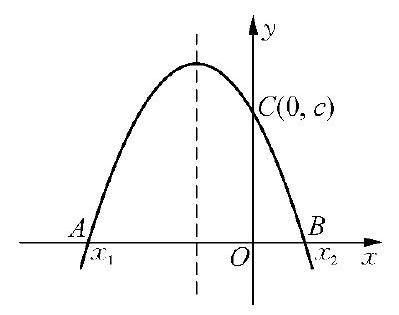
\includegraphics[max width=\textwidth, center]{2024_10_30_1bf34f7aeb61f11d11d3g-078}\\
$0<x_{2}$, 对称轴 $x=-\frac{b}{2 a} \leqslant 0$, 于是

\begin{align*}
\left|x_{1}\right|=\left|\frac{-b+\sqrt{b^{2}-4 a c}}{2 a}\right|=\frac{b-\sqrt{b^{2}-4 a c}}{2 a}=c
\end{align*}

则有

\begin{align*}
\frac{4 a c-b^{2}}{4 a} \geqslant c=\frac{b-\sqrt{b^{2}-4 a c}}{2 a} \geqslant-\frac{\sqrt{b^{2}-4 a c}}{2 a},
\end{align*}

故 $b^{2}-4 a c \geqslant 4$ ,当 $a=-1, b=0, c=1$ 时,等号成立。\\
所以 $b^{2}-4 a c$ 的最小值为 4 .\\
解法二 将 $\sqrt{b^{2}-4 a c}=b-2 a c$ 变形为 $\frac{-b+\sqrt{b^{2}-4 a c}}{2 a c}=-1(a c \neq 0)$,由此可得相应的一元二次方程 $a c x^{2}+b x+1=0$ 有实数根 $x=-1$, 所以 $a c-$ $b+1=0 \Rightarrow a c=b-1$, 故 $b^{2}-4 a c=b^{2}-4(b-1)=(b-2)^{2}$ 。

因为 $b \leqslant 0$, 所以当 $b=0$ 时, $b^{2}-4 a c$ 取得最小值, 最小值为 4 .\\
评注 当题目中的条件形如 $x=\frac{-b \pm \sqrt{b^{2}-4 a c}}{2 a}$ 时, 可联想一元二次方程的求根公式,通过构造一元二次方程来求解。\\
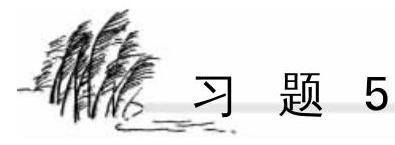
\includegraphics[max width=\textwidth, center]{2024_10_30_1bf34f7aeb61f11d11d3g-079}

1 如果 $|x| \leqslant \frac{\sqrt{2}}{2}$, 求函数 $y=-x^{2}+x+1$ 的最小值.\\
2 求函数 $y=2 x^{2}+4|x|-1$ 的最小值.\\
3 设 $x 、 y 、 z$ 为三个非负实数,且满足 $3 x+2 y+z=5,2 x+y-3 z=1$ 。求 $u=3 x+y-7 z$ 的最大值和最小值。\\
4 二次函数 $y=2 x^{2}+(a+1) x$ 的图象永远在二次函数 $y=x^{2}+x-b$ 的图象的上方, 求点 $(a, b)$ 所处的范围。\\
5 求函数 $f(x)=2 x+3-\sqrt{x+1}$ 的值域。\\
6 已知二次函数 $y=x^{2}+2(a+3) x+2 a+4$ 的图象与 $x$ 轴的两个交点的横坐标分别为 $\alpha 、 \beta$, 当实数 $a$ 变动时, 求 $(\alpha-1)^{2}+(\beta-1)^{2}$ 的最小值.\\
7 已知 $x^{2}+2 y^{2}=1$ ,求 $2 x+5 y^{2}$ 的最大值和最小值。\\
8 设 $a 、 b 、 c$ 是 $\triangle A B C$ 的三边长,二次函数 $y=\left(a-\frac{b}{2}\right) x^{2}-c x-a-\frac{b}{2}$ 在 $x=1$ 时取最小值 $-\frac{8}{5} b$, 试判断 $\triangle A B C$ 的形状.\\
9 求 $y=\frac{3 x^{2}+3 x+4}{x^{2}+x+1}$ 的最大值.\\
10 已知函数 $f(x)=a x^{2}-2 a x+1(a \neq 0)$ ,求 $f(x)$ 在闭区间 $[-1,2]$ 上的最值。

11 已知不等式 $a \leqslant x^{2}-4 x+6 \leqslant b$ 的解为 $a \leqslant x \leqslant b$, 求 $a$ 与 $b$ 的值.\\
12 已知函数 $y=f(x)$ 表示 $x-1$ 与 $\left|x^{2}-4 x+3\right|$ 两者中较大的一个,求在 $0 \leqslant x \leqslant 5$ 内函数 $f(x)-x$ 的取值范围。\\
13 把一张边长为 $a$ 的正方形纸 $A B C D$ 折起来,使 $B$点落在 $A D$ 上, 问 $B$ 点落在 $A D$ 什么位置上时, 使折起来的面积最小,并求出这最小面积的值。\\
14 设 $x 、 y$ 都是正整数,且使 $\sqrt{x-116}+\sqrt{x+110}=$ $y$ 。求 $y$ 的最大值。\\
15 已知函数 $f(x)=x^{2}+(k-4) x-2 k+4$ 。\\
(1)若对于任意 $k \in[-1,1], f(x)>0$ 恒成立,\\
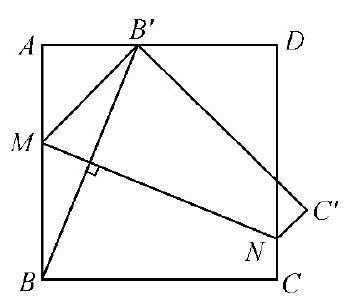
\includegraphics[max width=\textwidth, center]{2024_10_30_1bf34f7aeb61f11d11d3g-080}\\
(第 13 题)

求 $x$ 的取值范围;\\
(2)若对于任意 $k \in[-1,1], f(x)>0$ 恒成立, 求 $k$ 的取值范围.

有关一元二次方程的整数根问题,在这几年的竞赛中经常出现,而解决这类问题,通常都是通过讨论其判别式,利用根与系数的关系或因式分解等方法,然后通过检验确定答案。具体操作时,应视具体问题的特征,恰当地选择解题方法。

例1 设二次方程 $5 x^{2}-b x+2=0$ 有整数根 $m$ ,二次方程 $2 x^{2}-b x+$ $5=0$ 有整数根 $n$ ,且已知 $b \neq \pm 7$ ,则 $\frac{n}{m}$ 的值是 $\qquad$。\\
分析 若一元二次方程 $a x^{2}+b x+c=0$ 的两个根为 $x_{1} 、 x_{2}$, 则 $c x^{2}+$ $b x+a=0$ 的两个根为 $\frac{1}{x_{1}} 、 \frac{1}{x_{2}}$.

解 由题意 $m \neq n$ ,则二次方程 $5 x^{2}-b x+2=0$ 的两个根为 $m 、 \frac{1}{n}$ ,则由韦达定理知

\begin{align*}
m \cdot \frac{1}{n}=\frac{2}{5},
\end{align*}

所以

\begin{align*}
\frac{n}{m}=\frac{5}{2} .
\end{align*}

评注 请读者考虑一下, 若 $b= \pm 7$, 则结果会怎样?\\
例 2 设方程 $m x^{2}-(m-2) x+m-3=0$ 有整数解,试确定整数 $m$ 的值,并求出这时方程的所有整数解.

解 若 $m=0$, 则 $2 x-3=0$, 此时方程无整数根.\\
若 $m \neq 0$ ,考察方程的判别式

\begin{align*}
\begin{aligned}
\Delta & =(m-2)^{2}-4 m(m-3) \\
& =-3 m^{2}+8 m+4,
\end{aligned}
\end{align*}

注意到二次项系数为负,而方程有实数解,则

\begin{align*}
-3 m^{2}+8 m+4 \geqslant 0
\end{align*}

解得

\begin{align*}
\frac{4-2 \sqrt{7}}{3} \leqslant m \leqslant \frac{4+2 \sqrt{7}}{3} .
\end{align*}

因为 $m$ 是不为 0 的整数,故 $m$ 取 1、2、3.\\
当 $m=1$ 时,代入原方程,得解为: -2 和 1 ;\\
当 $m=2$ 时,方程无整数解;\\
当 $m=3$ 时, 方程有整数解为: 0 ;\\
综合可得, 当 $m=1$ 时, 有整数解 -2 和 1 ; 当 $m=3$ 时, 有整数解 0 。\\
评注 判别式法是处理一元二次方程有整数根的常用方法。当判别式的二次项系数为负时,一般通过解不等式得到关于参数的一个有限区间,再根据参数为整数,可以求得解。

例 3 试求所有的整数 $a$ ,使得关于 $x$ 的一元二次方程\\
$x^{2}-\sqrt{5 a^{2}-26 a-8} x-\left(a^{2}-4 a+9\right)=0$ 的两根皆为整数。\\
解 根据韦达定理得 $\sqrt{5 a^{2}-26 a-8}$ 为整数,则方程为整系数的一元二次方程,要使其根为整数,则其判别式为完全平方数。

则有

\begin{align*}
\begin{aligned}
& 5 a^{2}-26 a-8+4\left(a^{2}-4 a+9\right) \\
= & 9 a^{2}-42 a+28 \\
= & (3 a-7)^{2}-21 \\
= & b^{2},
\end{aligned}
\end{align*}

故 $(3 a-7)^{2}-b^{2}=21 \Rightarrow(3 a-7+b)(3 a-7-b)=21$ (其中 $b$ 为非负数).\\
所以

\begin{align*}
\begin{gathered}
\left\{\begin{array} { l } 
{ 3 a - 7 + b = 2 1 , } \\
{ 3 a - 7 - b = 1 , }
\end{array} \quad \left\{\begin{array}{l}
3 a-7+b=7, \\
3 a-7-b=3,
\end{array}\right.\right. \\
\left\{\begin{array}{l}
3 a-7+b=-1, \\
3 a-7-b=-21,
\end{array},\left\{\begin{array}{l}
3 a-7+b=-3, \\
3 a-7-b=-7
\end{array}\right.\right.
\end{gathered}
\end{align*}

因为 $a$ 为整数,则解得 $a=4$ 或 $a=6$ 。\\
当 $a=4$ 时, $\sqrt{5 a^{2}-26 a-8}$ 无意义, 所以当 $a=6$ ,此时方程为 $x^{2}-4 x-$ $21=0$ ,两个整数根为 7 和 -3 。

例 4 已知 $a$ 是正整数,如果关于 $x$ 的方程 $x^{3}+(a+17) x^{2}+(38-a) x-$ $56=0$ 的根都是整数,求 $a$ 的值及方程的整数根。

解 观察易知,方程有一个整数根 $x_{1}=1$ ,将方程的左边分解因式得

\begin{align*}
(x-1)\left[x^{2}+(a+18) x+56\right]=0,
\end{align*}

因为 $a$ 是正整数,所以关于 $x$ 的方程 $x^{2}+(a+18) x+56=0$ 的判别式\\
$\Delta=(a+18)^{2}-224>0$ ,它一定有两个不同的实数根,现要使根是整数,则它的判别式是一个完全平方数。

设 $(a+18)^{2}-224=k^{2}$ ( $k$ 为非负整数),则

\begin{align*}
(a+18)^{2}-k^{2}=224,
\end{align*}

即 $(a+18+k)(a+18-k)=224=112 \times 2=56 \times 4=28 \times 8$ 。\\
而 $a+18+k, a+18-k$ 的奇偶性相同,且 $a+18+k>18$ ,所以 $\left\{\begin{array}{l}a+18+k=112, \\ a+18-k=2,\end{array}\left\{\begin{array}{l}a+18+k=56, \\ a+18-k=4,\end{array} \quad\left\{\begin{array}{l}a+18+k=28, \\ a+18-k=8 .\end{array}\right.\right.\right.$

解得

\begin{align*}
\left\{\begin{array}{l}
a=39, \\
k=55,
\end{array}, \begin{array}{l}
a=12, \\
k=26,
\end{array},\left\{\begin{array}{l}
a=0 \\
k=10
\end{array}\right.\right.
\end{align*}

而 $a$ 是正整数,所以只可能是 $a=39$ 或 $a=12$.\\
当 $a=39$ 时, 方程化为 $x^{2}+57 x+56=0$ ,此时三个根为 $1,-1,-56$ 。\\
当 $a=12$ 时, 方程化为 $x^{2}+30 x+56=0$, 此时三个根为 $1,-2,-28$ 。\\
例 5 求所有实数 $k$ ,使二次方程 $k x^{2}+(k+1) x+(k-1)=0$ 的根都是整数。(江苏省数学竞赛)

解 (1)当 $k=0$ 时,原方程为 $x=1$ ,则 $k=0$ 满足题意。\\
(2)当 $k \neq 0$ 时,设两根为 $x_{1} 、 x_{2}$ ,则由韦达定理得

\begin{align*}
\left\{\begin{array}{l}
x_{1}+x_{2}=-\frac{k+1}{k}=-1-\frac{1}{k}, \\
x_{1} \cdot x_{2}=\frac{k-1}{k}=1-\frac{1}{k},
\end{array}\right.
\end{align*}

两式相减有

即

\begin{align*}
\begin{gathered}
x_{1}+x_{2}-x_{1} x_{2}=-2, \\
x_{1} x_{2}-\left(x_{1}+x_{2}\right)+1=3, \\
\left(x_{1}-1\right)\left(x_{2}-1\right)=3=1 \times 3
\end{gathered}
\end{align*}

因为 $x_{1} 、 x_{2}$ 都是整数,所以有

\begin{align*}
\begin{gathered}
\left\{\begin{array} { l } 
{ x _ { 1 } - 1 = 1 , } \\
{ x _ { 2 } - 1 = 3 , }
\end{array} \left\{\begin{array}{l}
x_{1}-1=3, \\
x_{2}-1=1,
\end{array}\right.\right. \\
\left\{\begin{array} { l } 
{ x _ { 1 } - 1 = - 1 , } \\
{ x _ { 2 } - 1 = - 3 , }
\end{array} \left\{\begin{array}{l}
x_{1}-1=-3, \\
x_{2}-1=-1,
\end{array}\right.\right.
\end{gathered}
\end{align*}

可得

\begin{align*}
x_{1}+x_{2}=6,
\end{align*}

或

\begin{align*}
x_{1}+x_{2}=-2 .
\end{align*}

当 $x_{1}+x_{2}=6$ 时, 即 $-1-\frac{1}{k}=6$, 得 $k=-\frac{1}{7}$ ;\\
当 $x_{1}+x_{2}=-2$ 时, 即 $-1-\frac{1}{k}=-2$, 得 $k=1$ 。\\
经检验,当 $k=1$ 或 $k=-\frac{1}{7}$ 时, $\Delta>0$ 。\\
所以 $k$ 的值为 $0,-\frac{1}{7}, 1$ 。\\
评注 该题如直接用求根公式讨论 $k$ 的值则较难解决,因为 $k$ 是实数,而不像前几题变量是整数。这里通过韦达定理,消去 $\frac{1}{k}$ 后剩下的都是整数,再利用质因数的分解就大大缩小了 $x_{1}+x_{2}$ 的范围,从而使问题得以顺利解决。

例 $6 a$ 是大于零的实数, 已知存在唯一的实数 $k$, 使得关于 $x$ 的方程

\begin{align*}
x^{2}+\left(k^{2}+a k\right) x+1999+k^{2}+a k=0
\end{align*}

的两根为素数,求 $a$ 的值。(全国初中数学竞赛)\\
分析 因 $a 、 k$ 都是实数,故用判别式较难解决,可考虑用韦达定理。\\
解 设方程的两根为 $x_{1} 、 x_{2}$ ,且 $x_{1} \leqslant x_{2}, x_{1} 、 x_{2}$ 均为素数,则

\begin{align*}
\left\{\begin{array}{l}
x_{1}+x_{2}=-k^{2}-a k \\
x_{1} \cdot x_{2}=1999+k^{2}+a k
\end{array}\right.
\end{align*}

两式相加,得

即

\begin{align*}
\begin{gathered}
x_{1}+x_{2}+x_{1} \cdot x_{2}=1999 \\
\left(x_{1}+1\right)\left(x_{2}+1\right)=2000=2^{4} \times 5^{3} .
\end{gathered}
\end{align*}

显然, $x_{1} \neq 2$ ,则 $x_{1}+1 、 x_{2}+1$ 都是偶数且 $x_{1}+1 \leqslant x_{2}+1$ ,于是有如下可能:

\begin{align*}
\begin{gathered}
\left\{\begin{array}{l}
x_{1}+1=2^{2}, \\
x_{2}+1=2^{2} \times 5^{3}
\end{array},\left\{\begin{array}{l}
x_{1}+1=2^{3}, \\
x_{2}+1=2 \times 5^{3},
\end{array}\right.\right. \\
\left\{\begin{array} { l } 
{ x _ { 1 } + 1 = 2 \times 5 , } \\
{ x _ { 2 } + 1 = 2 ^ { 3 } \times 5 ^ { 2 } , }
\end{array} \left\{\begin{array}{l}
x_{1}+1=2^{2} \times 5, \\
x_{2}+1=2^{2} \times 5^{2},
\end{array},\left\{\begin{array}{l}
x_{1}+1=2^{3} \times 5, \\
x_{2}+1=2 \times 5^{2} .
\end{array}\right.\right.\right.
\end{gathered}
\end{align*}

符合题意的只有 $\quad\left\{\begin{array}{l}x_{1}=3, \\ x_{2}=499,\end{array}\right.$\\
于是

\begin{align*}
x_{1}+x_{2}=-k^{2}-a k=3+499 .
\end{align*}

因为存在唯一的实数 $k$, 故方程 $k^{2}+a k+502=0$ 有两等根, 即

\begin{align*}
\Delta=a^{2}-4 \times 502=0
\end{align*}

解得

\begin{align*}
a=2 \sqrt{502} .
\end{align*}

例 7 求使关于 $x$ 的方程

\begin{align*}
(a+1) x^{2}-\left(a^{2}+1\right) x+2 a^{3}-6=0
\end{align*}

的根都为整数的所有整数 $a$.\\
解 (1) 当 $a+1=0$, 即 $a=-1$ 时, 得 $x=-4$, 满足题意.\\
(2) 当 $a+1 \neq 0$ 时, 设方程的两根为 $x_{1} 、 x_{2}$, 则

\begin{align*}
x_{1}+x_{2}=\frac{a^{2}+1}{a+1}=\frac{a^{2}-1+2}{a+1}=(a-1)+\frac{2}{a+1},
\end{align*}

要使方程的根都为整数,应满足 $a+1$ 是 2 的约数,就有 $a=-3 、-2 、 0 、 1$ 。\\
当 $a=-3$ 时, 方程无整数根;\\
当 $a=-2$ 时, 方程也无整数根;\\
当 $a=0$ 时, 两根为 $x_{1}=3, x_{2}=-2$;\\
当 $a=1$ 时, 两根为 $x_{1}=2, x_{2}=-1$ 。\\
所以, 原方程有整数根时, 整数 $a$ 的取值为 $-1 、 0 、 1$ 。\\
评注 此解法为分离参数法,它适合于参数与方程的根均为整数,且参数较易分离的情况。如此题把 $\frac{a^{2}+1}{a+1}$ 分解成 $(a-1)+\frac{2}{a+1}$ 的形式,再利用根为整数的条件进行讨论.

例8 已知方程 $x^{2}+(a-6) x+a=0(a \neq 0)$ 的两个根都是整数, 试求整数 $a$ 的值。

分析 本题按常规解法较繁,但若以 $a$ 为主元,用含 $x$ 的代数式表示 $a$ 的值, 利用整数的性质, 则可化繁为简.

解 原方程变形为 $(x+1) a=6 x-x^{2}$ 。\\
(1)当 $x=-1$ 时,代入原方程,易知不成立;\\
(2) 当 $x \neq-1$ 时, $a=\frac{6 x-x^{2}}{x+1}=\frac{-(x+1)^{2}+8(x+1)-7}{x+1}=-(x+$ 1) $+8-\frac{7}{x+1}$.

因为 $a 、 x$ 都是整数,则 $x+1= \pm 1$ 或 $x+1= \pm 7$, 解得 $x=0,-2,6$, - 8 .

把上述的 $x$ 值代入原方程,得 $a=0$ 或 $a=16$ 。\\
又因为 $a \neq 0$ ,所以整数 $a$ 的值为 16 。\\
评注 当一元二次方程的所含的字母为整数,且次数为一次时,可利用变换主元的方法来求解。本题也可以利用判别式来处理。

例 9 求满足方程 $x^{2}+y^{2}=2(x+y)+x y$ 的所有正整数 $x 、 y$ 。(上海高中理科班、数学班招生试题)

解 原方程整理成关于 $x$ 的一元二次方程

\begin{align*}
x^{2}-(y+2) x+y^{2}-2 y=0,
\end{align*}

这个方程要有正整数根,则它的判别式是完全平方数,即

\begin{align*}
\begin{aligned}
\Delta & =(y+2)^{2}-4\left(y^{2}-2 y\right) \\
& =-3 y^{2}+12 y+4 \\
& =16-3(y-2)^{2}
\end{aligned}
\end{align*}

为完全平方,且

\begin{align*}
0 \leqslant 16-3(y-2)^{2} \leqslant 16
\end{align*}

当 $16-3(y-2)^{2}=0$ 时,无正整数解;\\
当 $16-3(y-2)^{2}=1$ 时,无正整数解;\\
当 $16-3(y-2)^{2}=4$ 时, $y=4$ ;\\
当 $16-3(y-2)^{2}=9$ 时,无正整数解;\\
当 $16-3(y-2)^{2}=16$ 时, $y=2$ 。\\
于是得到正整数解为

\begin{align*}
\left\{\begin{array}{l}
x=4, \\
y=4,
\end{array},\left\{\begin{array}{l}
x=2, \\
y=4,
\end{array},\left\{\begin{array}{l}
x=4 \\
y=2
\end{array}\right.\right.\right.
\end{align*}

例 10 已知 $p$ 为素数,使二次方程

\begin{align*}
x^{2}-2 p x+p^{2}-5 p-1=0
\end{align*}

的两根都是整数,求出 $p$ 的所有可能值。(上海初中数学竞赛)\\
解 因为整系数的二次方程有整数根,则其判别式为完全平方数,即

\begin{align*}
\begin{aligned}
\Delta & =4 p^{2}-4\left(p^{2}-5 p-1\right) \\
& =4(5 p+1)
\end{aligned}
\end{align*}

为完全平方,从而 $5 p+1$ 为完全平方。\\
令 $5 p+1=n^{2}$, 因为 $p \geqslant 2$, 故 $n \geqslant 4$ 且 $n$ 为正整数,则有

\begin{align*}
5 p=n^{2}-1=(n+1)(n-1)
\end{align*}

故 $n+1 、 n-1$ 中至少有一个是 5 的倍数, 即

\begin{align*}
n=5 k \pm 1 \text { ( } k \text { 为正整数). }
\end{align*}

因此把 $n=5 k \pm 1$ 代入 $5 p+1=n^{2}$ 中得

整理得

\begin{align*}
\begin{aligned}
5 p+1 & =25 k^{2} \pm 10 k+1, \\
p & =k(5 k \pm 2) .
\end{aligned}
\end{align*}

因 $p$ 为素数, 且 $5 k \pm 2>1$, 则有

从而

\begin{align*}
p=3 \text { 或 } p=7 \text {. }
\end{align*}

当 $p=3$ 时, 原方程为

解得

\begin{align*}
\begin{gathered}
x^{2}-6 x-7=0, \\
x_{1}=-1 \text { 或 } x_{2}=7 .
\end{gathered}
\end{align*}

当 $p=7$ 时, 原方程为

解得

\begin{align*}
\begin{gathered}
x^{2}-14 x+13=0, \\
x_{1}=1 \text { 或 } x_{2}=13 . \\
p=3 \text { 或 } p=7 .
\end{gathered}
\end{align*}

所以\\
例11 已知 $p 、 q$ 都是素数, 且使得关于 $x$ 的一元二次方程 $x^{2}-(8 p-$ $10 q) x+5 p q=0$ 至少有一个正整数根,求所有的素数对 $(p, q)$ 。

分析 虽然题目要求至少有一个整数根,但根据韦达定理,知若有一个正整数根, 则另一根也必为正整数, 所以等价于两根都是正整数根时, 求所有的素数对 $(p, q)$ 。

解 设一元二次方程的两个根为 $x_{1} 、 x_{2}$, 则根据根与系数的关系得:

\begin{align*}
\left\{\begin{array}{l}
x_{1}+x_{2}=8 p-10 q, \\
x_{1} \cdot x_{2}=5 p q .
\end{array}\right.
\end{align*}

从上可知,若方程有一个正整数根,则另一根也必为正整数。\\
于是根据 $x_{1} \cdot x_{2}=5 p q$, 而 $p 、 q$ 都是素数,知 $x_{1} 、 x_{2}$ 有如下四种可能:

\begin{align*}
\left\{\begin{array} { l } 
{ x _ { 1 } = 1 , } \\
{ x _ { 2 } = 5 p q , }
\end{array} \quad \left\{\begin{array} { l } 
{ x _ { 1 } = 5 , } \\
{ x _ { 2 } = p q , }
\end{array} \left\{\begin{array}{l}
x_{1}=p, \\
x_{2}=5 q,
\end{array},\left\{\begin{array}{l}
x_{1}=q \\
x_{2}=5 p
\end{array}\right.\right.\right.\right.
\end{align*}

将上面四种情况分别代入 $x_{1}+x_{2}=8 p-10 q$.\\
(1)当 $x_{1}=1, x_{2}=5 p q$ 时,得

化为

\begin{align*}
5 q(p+2)-8(p+2)+16+1=0,
\end{align*}

即

\begin{align*}
(p+2)(8-5 q)=17=1 \times 17
\end{align*}

易知不存在素数对 $(p, q)$ 。\\
(2)当 $x_{1}=5, x_{2}=p q$ 时,得

\begin{align*}
5+p q=8 p-10 q
\end{align*}

化为

\begin{align*}
(8-q)(10+p)=85=5 \times 17=1 \times 85
\end{align*}

得

\begin{align*}
\left\{\begin{array} { l } 
{ q = 3 , } \\
{ p = 7 , }
\end{array} \text { 或 } \left\{\begin{array}{l}
q=7, \\
p=75 .
\end{array}\right.\right. \text { 舍去) }
\end{align*}

(3)当 $x_{1}=p, x_{2}=5 q$ 时,得

\begin{align*}
p+5 q=8 p-10 q
\end{align*}

化为

\begin{align*}
7 p=15 q
\end{align*}

得

\begin{align*}
\left\{\begin{array}{l}
p=15, \\
q=7 .
\end{array}\right. \text { (舍去) }
\end{align*}

(4)当 $x_{1}=q, x_{2}=5 p$ 时,得

\begin{align*}
5 p+q=8 p-10 q
\end{align*}

化为

\begin{align*}
3 p=11 q,
\end{align*}

得

\begin{align*}
\left\{\begin{array}{l}
p=11 \\
q=3
\end{array}\right.
\end{align*}

综上, 符合条件的所有素数对为 $(7,3),(11,3)$ 。\\
例12 已知关于 $x$ 的方程 $4 x^{2}-8 n x-3 n=2$ 和 $x^{2}-(n+3) x-2 n^{2}+$ $2=0$ ,问是否存在这样的 $n$ 值,使第一个方程的两个实数根的差的平方等于第二个方程的一整数根?若存在,求出这样的 $n$ 值;若不存在,请说明理由。 (湖北省初中数学竞赛)

解 设方程

\begin{align*}
4 x^{2}-8 n x-3 n-2=0
\end{align*}

的两个根为 $x_{1} 、 x_{2}$ ,则由韦达定理,得

\begin{align*}
\left\{\begin{array}{l}
x_{1}+x_{2}=2 n \\
x_{1} \cdot x_{2}=\frac{-(3 n+2)}{4}
\end{array}\right.
\end{align*}

故

\begin{align*}
\begin{aligned}
& \left(x_{1}-x_{2}\right)^{2} \\
= & \left(x_{1}+x_{2}\right)^{2}-4 x_{1} x_{2}, \\
= & 4 n^{2}+3 n+2 .
\end{aligned}
\end{align*}

又对方程 $x^{2}-(n+3) x-2 n^{2}+2=0$ 因式分解,可得

\begin{align*}
[x-(2 n+2)][x+(n-1)]=0,
\end{align*}

解得两根为 $2 n+2$ 或 $1-n$ 。\\
当 $2 n+2$ 为整数时,则

解得

\begin{align*}
\begin{gathered}
4 n^{2}+3 n+2=2 n+2, \\
n=0 \text { 或 } n=-\frac{1}{4} .
\end{gathered}
\end{align*}

若 $n=0$, 则 $2 n+2=2$, 满足题意;\\
若 $n=-\frac{1}{4}$ ,则 $2 n+2=\frac{3}{2}$ 不是整数,舍去。\\
当 $1-n$ 为整数时,则

解得

\begin{align*}
\begin{gathered}
4 n^{2}+3 n+2=1-n, \\
n=-\frac{1}{2} .
\end{gathered}
\end{align*}

若 $n=-\frac{1}{2}$ ,则 $1-n=\frac{3}{2}$ 不是整数,舍去。\\
综上知,当 $n=0$ 时,第一个方程的两个实数根的差的平方等于第二个方程的一整数根。

例13 已知 $a 、 b$ 都是正整数,试问:关于 $x$ 的方程 $x^{2}-a b x+\frac{1}{2}(a+b)=$ 0 是否有两个整数解?如果有,请把它们求出来;如果没有,请说明理由。

解 不妨设 $a \leqslant b$ ,且方程的两个整数根为 $x_{1} 、 x_{2}\left(x_{1} \leqslant x_{2}\right)$ ,则根据韦\\
达定理有

\begin{align*}
\left\{\begin{array}{l}
x_{1}+x_{2}=a b, \\
x_{1} \cdot x_{2}=\frac{1}{2}(a+b),
\end{array}\right.
\end{align*}

有

\begin{align*}
x_{1}+x_{2}-x_{1} x_{2}=a b-\frac{1}{2} a-\frac{1}{2} b,
\end{align*}

整理得

\begin{align*}
4\left(x_{1}-1\right)\left(x_{2}-1\right)+(2 a-1)(2 b-1)=5 .
\end{align*}

因为 $a 、 b$ 都是正整数,则 $x_{1} 、 x_{2}$ 也都是正整数,于是有

故

\begin{align*}
\begin{aligned}
& x_{1}-1 \geqslant 0, x_{2}-1 \geqslant 0,2 a-1 \geqslant 1,2 b-1 \geqslant 1, \\
& \left\{\begin{array} { l } 
{ ( x _ { 1 } - 1 ) ( x _ { 2 } - 1 ) = 0 , } \\
{ ( 2 a - 1 ) ( 2 b - 1 ) = 5 , }
\end{array} \text { 或 } \left\{\begin{array}{l}
\left(x_{1}-1\right)\left(x_{2}-1\right)=1, \\
(2 a-1)(2 b-1)=1 .
\end{array}\right.\right.
\end{aligned}
\end{align*}

(1) 当 $\left\{\begin{array}{l}\left(x_{1}-1\right)\left(x_{2}-1\right)=0, \\ (2 a-1)(2 b-1)=5\end{array}\right.$ 时, 因为 $a 、 b$ 都是正整数,且 $a \leqslant b$, 所以 $\left\{\begin{array}{l}a=1, \\ b=3,\end{array}\right.$ 此时一元二次方程的两个整数解为 $\left\{\begin{array}{l}x_{1}=1, \\ x_{2}=2 .\end{array}\right.$\\
(2) 当 $\left\{\begin{array}{l}\left(x_{1}-1\right)\left(x_{2}-1\right)=1, \\ (2 a-1)(2 b-1)=1\end{array}\right.$ 时, 因为 $a 、 b$ 都是正整数, 所以 $\left\{\begin{array}{l}a=1, \\ b=1,\end{array}\right.$此时一元二次方程为 $x^{2}-x+1=0$ ,方程无解。

综上所述,当且仅当 $a=1, b=3$ 时,方程组有整数解,解为 $x_{1}=1$ , $x_{2}=2$ 。

评注 本题关键是利用韦达定理建立了一个关于整数根 $x_{1} 、 x_{2}$ 和变量 $a 、 b$ 的一个方程,即 $4\left(x_{1}-1\right)\left(x_{2}-1\right)+(2 a-1)(2 b-1)=5$ ,再利用整数的性质来处理。

例14 某顾客有钱 10 元,第一次在商店买 $x$ 件小商品花去 $y$ 元,第二次再去买该小商品时,发现每打( 12 件)降低 0.8 元,他比第一次多买了 10 件,花去 2 元。问他第一次买的小商品是多少件?( $x, y$ 为正整数)

分析 通过分析题意,可以列出方程 $\frac{y}{x}-\frac{2}{x+10}=\frac{0.8}{12}$ ,这样就转化为求方程的正整数解.

解 由题意,得方程

\begin{align*}
\frac{y}{x}-\frac{2}{x+10}=\frac{0.8}{12}
\end{align*}

整理成关于 $x$ 的一元二次方程为

\begin{align*}
x^{2}+(40-15 y) x-150 y=0
\end{align*}

现求正整数 $y$ 为何值时方程有正整数解. 考察方程的判别式,有

\begin{align*}
\begin{aligned}
\Delta & =(40-15 y)^{2}+4 \times 150 y \\
& =25\left[(3 y-4)^{2}+48\right],
\end{aligned}
\end{align*}

设 $(3 y-4)^{2}+48=n^{2}(n>0, n$ 为正整数), 移项后因式分解,可得

\begin{align*}
(n+3 y-4)(n-3 y+4)=48=2^{4} \times 3
\end{align*}

又 $(n+3 y-4)$ 与 $(n-3 y+4)$ 同奇偶, 所以有以下几种情况:

\begin{align*}
\left\{\begin{array}{l}
n+3 y-4=2^{3} \times 3  \tag{1}\\
n-3 y+4=2
\end{array}\right.
\end{align*}

\begin{align*}
\left\{\begin{array}{l}
n+3 y-4=2^{3}  \tag{2}\\
n-3 y+4=2 \times 3
\end{array}\right.
\end{align*}

\begin{align*}
\left\{\begin{array}{l}
n+3 y-4=2^{2} \times 3  \tag{3}\\
n-3 y+4=2^{2}
\end{array}\right.
\end{align*}

\begin{align*}
\left\{\begin{array}{l}
n+3 y-4=2  \tag{4}\\
n-3 y+4=2^{3} \times 3
\end{array}\right.
\end{align*}

\begin{align*}
\left\{\begin{array}{l}
n+3 y-4=2 \times 3  \tag{5}\\
n-3 y+4=2^{3}
\end{array}\right.
\end{align*}

\begin{align*}
\left\{\begin{array}{l}
n+3 y-4=2^{2}  \tag{6}\\
n-3 y+4=2^{2} \times 3
\end{array}\right.
\end{align*}

由题意 $y 、 n$ 为正整数,可知满足题意的有(1)和(5)两种情况,解得

\begin{align*}
\left\{\begin{array} { l } 
{ n = 1 3 , } \\
{ y = 5 , }
\end{array} \text { 或 } \left\{\begin{array}{l}
n=7, \\
y=1,
\end{array}\right.\right.
\end{align*}

代入原方程得

\begin{align*}
x=50 \text { 或 } x=5 \text {. }
\end{align*}

即他第一次买的小商品是 50 件或 5 件。\\
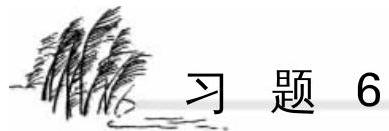
\includegraphics[max width=\textwidth, center]{2024_10_30_1bf34f7aeb61f11d11d3g-091}

1 已知 $n$ 为正整数, 方程 $x^{2}-(\sqrt{3}+1) x+\sqrt{3} n-6=0$ 有一个整数根, 求 $n$的值。\\
2 设 $m$ 为整数,且 $4<m<40$ ,又方程 $x^{2}-2(2 m-3) x+4 m^{2}-14 m+$ $8=0$ 有两个整数根,求 $m$ 的值及方程的根。

3 已知方程 $x^{2}-(k+3) x+k^{2}=0$ 的根都是整数,求整数 $k$ 的值及方程的根。\\
4 试确定一切有理数 $r$ ,使得关于 $x$ 的方程 $r x^{2}+(r+2) x+3 r-2=0$ 有根且只有整数根。\\
5 当 $x$ 为何有理数时,代数式 $9 x^{2}+23 x-2$ 的值恰为两个连续正偶数的乘积?\\
6 试求出所有这样的正整数 $a$ ,使得二次方程 $a x^{2}+2(2 a-1) x+4(a-$ $3)=0$ 至少有一个整数根。\\
77 设 $\alpha$ 为整数,若存在整数 $b$ 和 $c$ ,使得 $(x+\alpha)(x-15)-25=(x+b) \cdot$ $(x+c)$ 成立,求 $\alpha$ 可取的值。\\
8 以关于 $m$ 的方程 $m^{2}+(k-4) m+k=0$ 的最大整数根为直径作 $\odot O, P$为 $\odot O$ 外一点,过 $P$ 作切线 $P A$ 和割线 $P B C, A$ 为切点,这时发现 $P A$ 、 $P B 、 P C$ 都是正整数,且 $P B 、 P C$ 都不是合数。求 $P A 、 P B 、 P C$ 的长.\\
9 关于 $x$ 的一元二次方程 $m x^{2}-4 x+4=0$ 与方程 $x^{2}-4 m x+4 m^{2}-$ $4 m-5=0$ 的根都是整数,求 $m$ 的值。\\
10 已知关于 $x$ 的方程 $\left(m^{2}-1\right) x^{2}-3(3 m-1) x+18=0$ 有两个正整数根 $(m$是整数), $\triangle A B C$ 的三边 $a 、 b 、 c$ 满足 $c=2 \sqrt{3}, m^{2}+a^{2} m-8 a=0, m^{2}+$ $b^{2} m-8 b=0$.\\
(1) 求 $m$ 的值;\\
(2) 求 $\triangle A B C$ 的面积.

11 求方程组 $\left\{\begin{array}{l}x+y+z=3, \\ x^{3}+y^{3}+z^{3}=3\end{array}\right.$ 的所有整数解.\\
12 已知 $n$ 为正整数,且关于 $x$ 的一元二次方程 $(n-1)^{2} x^{2}-5 n(n-1) x+$ $\left(6 n^{2}-n-1\right)=0$ 至少有一个整数根,求所有 $n$ 的值的和。\\
13 设 $a$ 是正整数,如果二次函数 $y=2 x^{2}+(2 a+23) x+10-7 a$ 和反比例函数 $y=\frac{11-3 a}{x}$ 的图象有公共整点(横、纵坐标都是整点的点),求 $a$ 的值和对应的公共整点。\\
14 已知 $n$ 为自然数,关于 $x$ 的一元二次方程 $2 x^{2}-8 n x+10 x-n^{2}+35 n-$ $76=0$ 的两根为素数,试解此方程。\\
15 用正方形的地砖不重叠、无缝隙地铺满一块地,选用边长为 $x \mathrm{~cm}$ 规格的地砖恰需 $n$ 块;若选用边长为 $y \mathrm{~cm}$ 规格的地砖,则要比前一种刚好多用 124 块。已知 $x 、 y 、 n$ 都是自然数,且 $x 、 y$ 互质,求这块地的面积。

\section*{函数的应用}
函数是中学代数的基本内容之一,它既简单又具有丰富的内涵和外延.一次函数、反比例函数和二次函数是最基本的初等函数,可以以它们为素材来研究函数的性质,还可以建立起函数、方程、不等式之间的有机联系(大家知道,函数中的 $y$ 在变化中变成 0 ,函数就成了方程;其中的等号变成不等号,函数就成了不等式)。同时有关函数的内容又与实际问题的应用联系非常密切,与近、现代数学的发展紧密联系,是学生进入高校继续深造的重要基础知识。

学习函数, 重要的是从两个方面入手: 一是解析式, 二是函数的图象特征. 从解析式出发,可以进行纯粹的代数推理,这种代数推理、论证的能力可以反映出一个人的基本数学素养;从图象特征出发,可以实现数与形的自然结合,这是数学中的一种非常重要的思想方法。

例1 如果关于 $x$ 的方程 $|x-1|+|x+1|=a$ 有实数根,求实数 $a$ 的取值范围。

解 我们考查函数 $y=|x-1|+|x+1|$, 得 $y= \begin{cases}2 x, & x \geqslant 1, \\ 2, & -1<x<1, \\ -2 x, & x \leqslant-1,\end{cases}$\\
根据函数图象,知当 $a \geqslant 2$ 时,该方程有解。\\
评注 处理绝对值的题目,我们往往利用绝对值的定义把绝对值去掉,本题去绝对值的方法叫做零点分段法,即先求出每个绝对值的零点: $x=1$ 和 $x=-1$, 这两个零点就把数轴分成了 3 段, 然后对每段进行讨论, 转化为一个分段函数,从而解决问题。

例 2 已知 $a 、 b 、 c$ 为整数, 且 $a+b=2006, c-a=2005$, 若 $a<b$, 求 $a+b+c$ 的最大值.

解 由 $a+b=2006, c-a=2005$, 得 $a+b+c=a+4011$. 令 $y=$ $a+b+c$, 则转化为关于 $a$ 的一次函数, 即 $y=a+4011$. 又因为 $a<b, a$ 为整数,根据 $a+b=2006$ 得 $a$ 的最大值为 1002 。

所以 $a+b+c \leqslant 1002+4011=5013$ ,即 $a+b+c$ 的最大值为 5013 。\\
评注 本题的关键是转化为关于 $a$ 的一次函数来求,本题用"主元法"实现这一目的。

例3 某航空部队进行射击训练示意图如图71 所示,在地面 $O 、 A$ 两个观察点测得空中固定目标 $C$的仰角为 $\alpha$ 和 $\beta, O A=1 \mathrm{~km}, \tan \alpha=\frac{9}{28}, \tan \beta=\frac{3}{8}$,位于 $O$ 点正上方 $\frac{5}{3} \mathrm{~km} D$ 处的直升机向目标 $C$ 发射防空导弹,设导弹运行达到距地面最大高度 3 km 时,相应的水平距离约为 4 km (即图中的 $E$ 点),若导弹\\
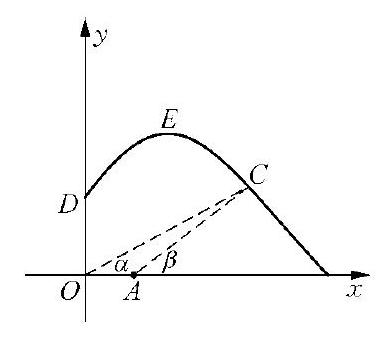
\includegraphics[max width=\textwidth, center]{2024_10_30_1bf34f7aeb61f11d11d3g-094}

图7-1

运行轨道为一条抛物线,问:按此轨道运行的导弹能否击中目标 $C$ ?

分析 根据题意,我们先建立直角坐标系,求出导弹运行轨迹的解析式,然后判断 $C$ 点坐标满足不满足解析式。

解 以 $O$ 为坐标原点建立直角坐标系, 则抛物线的顶点坐标为 $(4,3)$, 且过点 $\left(0, \frac{5}{3}\right)$, 设抛物线的解析式为 $y=a(x-4)^{2}+3$.

把 $D\left(0, \frac{5}{3}\right)$ 代入上式得

\begin{align*}
\frac{5}{3}=a(0-4)^{2}+3
\end{align*}

解得

\begin{align*}
a=-\frac{1}{12}
\end{align*}

所以

\begin{align*}
y=-\frac{1}{12} x^{2}+\frac{2}{3} x+\frac{5}{3}
\end{align*}

设 $C\left(x_{0}, y_{0}\right)$, 过点 $C$ 作 $C B \perp x$ 轴于点 $B$.\\
在 Rt $\triangle O B C$ 和 Rt $\triangle A B C$ 中, $O A=1, \tan \alpha=\frac{y_{0}}{x_{0}}=\frac{9}{28}, \tan \beta=$ $\frac{y_{0}}{x_{0}-1}=\frac{3}{8}$ ,则有

得

\begin{align*}
\frac{9}{28} x_{0}=\frac{3}{8}\left(x_{0}-1\right)
\end{align*}

\begin{align*}
x_{0}=7
\end{align*}

即 $C\left(7, \frac{9}{4}\right)$ 。\\
把 $x=7$ 代入抛物线方程 $y=-\frac{1}{12} x^{2}+\frac{2}{3} x+\frac{5}{3}$, 得 $y=\frac{9}{4}$.\\
故点 $C$ 在抛物线上,即导弹能击中目标 $C$.\\
例 4 (1)证明:若 $x$ 取任意整数时,二次函数 $y=a x^{2}+b x+c$ 总取整数值,那么 $2 a 、 a-b 、 c$ 都是整数;\\
(2)写出上述命题的逆命题,判断真假,并证明你的结论.\\
分析 本题主要研究当 $x 、 y$ 都是整数时,系数的代数式 $2 a 、 a-b 、 c$ 所表示的意义,一般解决这类问题从特殊值出发。

证明 (1)因为 $x$ 取任意整数时,二次函数 $y=a x^{2}+b x+c$ 总取整数值,则当 $x=0$ 时, $y=c$ 也为整数,故 $c$ 为整数;

当 $x=-1$ 时, $y=a-b+c$ 为整数,则 $a-b=y-c$ ,故 $a-b$ 为整数;\\
当 $x=1$ 时, $y=a+b+c=2 a-(a-b)+c$ 为整数,则 $2 a=y+(a-$ $b)-c$ ,故 $2 a$ 为整数。

因此 $2 a 、 a-b 、 c$ 都是整数。\\
(2)所求的逆命题为:若 $2 a 、 a-b 、 c$ 都是整数,那么 $x$ 取任意整数时,二次函数 $y=a x^{2}+b x+c$ 总取整数值。

这是一个真命题,下面给出两种证明方法:\\
证明一 若 $2 a 、 a-b 、 c$ 都是整数,则二次函数可化为

\begin{align*}
\begin{aligned}
y & =a x^{2}+b x+c=a x^{2}+a x-a x+b x+c \\
& =a x(x+1)-(a-b) x+c \\
& =2 a \frac{1}{2} x(x+1)-(a-b) x+c
\end{aligned}
\end{align*}

当 $x$ 取整数时, $x(x+1)$ 是连续的两个整数相乘,一定为偶数,则 $\frac{1}{2} x(x+$ $1)$ 为整数, 所以 $2 a \frac{1}{2} x(x+1)$ 是整数; 又因为 $a-b 、 c$ 为整数, 则 $-(a-b) x+$ $c$ 是整数。

因此当 $x$ 取任意整数时,二次函数 $y=a x^{2}+b x+c$ 总是整数.\\
证明二 当 $x$ 为偶数时,设 $x=2 k$ 。\\
因为 $2 a 、 a-b 、 c$ 为整数,则 $2 b=2 a-2(a-b)$ 也为整数,有

\begin{align*}
y=a(2 k)^{2}+b(2 k)+c=2 a \cdot 2 k^{2}+2 b \cdot k+c
\end{align*}

故函数值为整数;

当 $x$ 为奇数时, 设 $x=2 k-1$.

\begin{align*}
\begin{aligned}
y & =a(2 k-1)^{2}+b(2 k-1)+c \\
& =2 a \cdot\left(2 k^{2}-2 k\right)+2 b \cdot k+(a-b)+c
\end{aligned}
\end{align*}

每一项都是整数,故函数值为整数。\\
因此当 $x$ 取任意整数时,二次函数 $y=a x^{2}+b x+c$ 总是整数.\\
例 5 通过实验研究,专家们发现:初中学生注意力指标数是随着老师讲课时间变化而变化的,讲课开始时,学生兴趣激增,中间有一段时间兴趣保持平稳状态,随后开始分散。学生注意力指标数 $y$ 随时间 $x$ (分钟)变化函数图象如图 $7-2$ 所示( $y$ 越大表示越集中)。当 $0 \leqslant x \leqslant 10$时,图象是抛物线一部分,当 $10 \leqslant x \leqslant 20$ 和 $20 \leqslant x \leqslant 40$ 时,图象是线段。\\
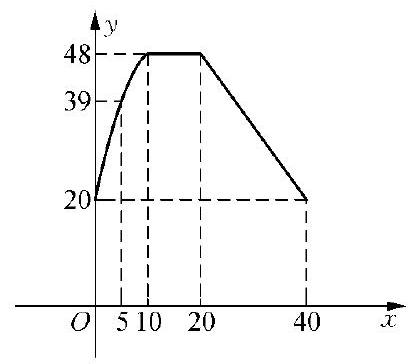
\includegraphics[max width=\textwidth, center]{2024_10_30_1bf34f7aeb61f11d11d3g-096}

图7-2\\
(1)当 $0 \leqslant x \leqslant 10$ 时,求指标数 $y$ 与时间 $x$ 函数关系式;\\
(2)一道数学综合题,需要讲解 24 分钟。问老师能否经过适当安排,使学生听这道题时,指标数都不低于 36 。

解 (1)当 $0 \leqslant x \leqslant 10$ 时,设抛物线的函数关系式为 $y=a x^{2}+b x+c$ ,由于它的图象经过点 $(0,20),(5,39),(10,48)$ ,所以有

\begin{align*}
\left\{\begin{array}{l}
c=20 \\
25 a+5 b+c=39 \\
100 a+10 b+c=48
\end{array}\right.
\end{align*}

解得

\begin{align*}
a=-\frac{1}{5}, b=\frac{24}{5}, c=20
\end{align*}

所以函数关系式为: $y=-\frac{1}{5} x^{2}+\frac{24}{5} x+20(0 \leqslant x \leqslant 10)$.\\
(2)当 $20 \leqslant x \leqslant 40$ 时, $y=-\frac{7}{5} x+76$ 。\\
令 $y=36$, 得

解为

\begin{align*}
\begin{aligned}
& 36=-\frac{7}{5} x+76 \\
& x=\frac{200}{7}=28 \frac{4}{7}
\end{aligned}
\end{align*}

当 $0 \leqslant x \leqslant 10$ 时,令 $y=36$ ,得

\begin{align*}
\begin{aligned}
36 & =-\frac{1}{5} x^{2}+\frac{24}{5} x+20, \\
x & =4, x=20 \text { (舍去). }
\end{aligned}
\end{align*}

因为 $28 \frac{4}{7}-4=24 \frac{4}{7}>24$ ,所以老师可以经过适当安排,在学生注意力指标数不低于 36 的情况下,讲授完这道竞赛题。

评注 此题综合性强,把二次函数、一次函数有机地与实际问题融合在一起,并与高中的分段函数相联系,起到承前启后的作用。

例 6 求方程 $6 x-3[x]+7=0$ 的解。\\
解 方程 $6 x-3[x]+7=0$ 可写为 $[x]=\frac{6 x+7}{3}$, 又因为 $x-1<$ $[x] \leqslant x$, 则有 $x-1<\frac{6 x+7}{3} \leqslant x$.

解此不等式组得

\begin{align*}
-\frac{10}{3}<x \leqslant-\frac{7}{3},
\end{align*}

故

\begin{align*}
[x]=-4 \text { 或 }-3 .
\end{align*}

即有

\begin{align*}
\frac{6 x+7}{3}=-4 \text { 或 } \frac{6 x+7}{3}=-3 \text {, }
\end{align*}

解得

\begin{align*}
x=-\frac{19}{6} \text { 或 } x=-\frac{8}{3} .
\end{align*}

经检验: $x=-\frac{19}{6}$ 或 $x=-\frac{8}{3}$ 都是原方程的解.\\
例7 求方程 $x^{2}-2[x]-3=0$ 的解。\\
解 由题所给方程得

\begin{align*}
[x]=\frac{x^{2}-3}{2},
\end{align*}

而 $x-1<[x] \leqslant x$, 则有

即等价于

\begin{align*}
x-1<\frac{x^{2}-3}{2} \leqslant x
\end{align*}

\begin{align*}
\left\{\begin{array}{l}
x^{2}-2 x-3 \leqslant 0 \\
x^{2}-2 x-1>0
\end{array}\right.
\end{align*}

解得

\begin{align*}
-1 \leqslant x<1-\sqrt{2} \text { 或 } 1+\sqrt{2}<x \leqslant 3 \text {. }
\end{align*}

因此 $[x]$ 只可能取值为 $-1,2,3$.

当 $[x]=-1$ 时, $\frac{x^{2}-3}{2}=-1$, 得 $x=-1$ ;\\
当 $[x]=2$ 时, $\frac{x^{2}-3}{2}=2$, 得 $x=\sqrt{7}$ ;\\
当 $[x]=3$ 时, $\frac{x^{2}-3}{2}=3$, 得 $x=3$.\\
经检验: $x=-1, \sqrt{7}, 3$ 都是方程的解。\\
评注 上述解题方法如出一辙,其解题步骤可以概括为:(1)从原方程中解出 $[x]$ (用含 $x$ 的代数式表示);(2)代入不等式组 $x-1<[x] \leqslant x$ ,求出 $x$的范围,得到 $[x]$ 的可能取值;(3)将这些可能值分别代入原方程求解;(4)检验求出的值是否满足题意。

例8 如图 7-3 所示, 已知点 $M 、 N$ 的坐标分别为 $(0,1) 、(0,-1)$ ,点 $P$ 是抛物线 $y=$ $\frac{1}{4} x^{2}$ 上的一个动点。(全国初中数学联赛)\\
(1) 判断以点 $P$ 为圆心, $P M$ 为半径的圆与直线 $y=-1$ 的位置关系;\\
(2)设直线 $P M$ 与抛物线 $y=\frac{1}{4} x^{2}$ 的另一\\
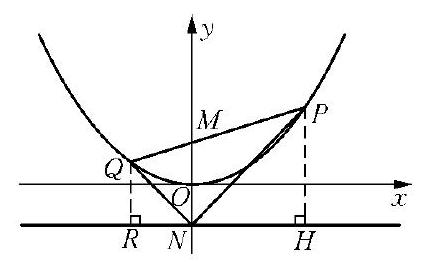
\includegraphics[max width=\textwidth, center]{2024_10_30_1bf34f7aeb61f11d11d3g-098}

图7-3

个交点为 $Q$, 连结 $N P 、 N Q$, 求证: $\angle P N M=\angle Q N M$ 。

分析 (1)可先根据抛物线的解析式设出 $P$ 点的坐标,可得出线段 $P M$的长的表达式,从而可以判断出 $P M$ 和 $P$ 到 $y=-1$ 的距离的两个式子是否相等。\\
(2)要证明这两个角相等,可以通过构建相似三角形来解决.\\
解 (1) 设点 $P$ 的坐标为 $\left(x_{0}, \frac{1}{4} x_{0}^{2}\right)$, 则

\begin{align*}
|P M|=\sqrt{x_{0}^{2}+\left(\frac{1}{4} x_{0}^{2}-1\right)^{2}}=\sqrt{\left(\frac{1}{4} x_{0}^{2}+1\right)^{2}}=\frac{1}{4} x_{0}^{2}+1
\end{align*}

又因为点 $P$ 到直线 $y=-1$ 的距离为 $\frac{1}{4} x_{0}^{2}-(-1)=\frac{1}{4} x_{0}^{2}+1$, 所以以点 $P$ 为圆心, $P M$ 为半径的圆与直线 $y=-1$ 相切。\\
(2)分别过点 $P 、 Q$ 作直线 $y=-1$ 的垂线,垂足分别为 $H 、 R$ 。\\
由(1)的结论可知 $P M=P H$ ,同理可得 $Q M=Q R$ 。\\
因为 $P H 、 M N 、 Q R$ 都垂直于 $y=-1$, 则有 $P H / / M N / / Q R$.\\
于是得 $\frac{Q M}{R N}=\frac{M P}{N H}$, 即 $\frac{Q R}{R N}=\frac{P H}{N H}$, 所以 Rt $\triangle P H N$ 相似于 Rt $\triangle Q R N$,

从而 $\angle P N M=\angle Q N M$.\\
例 9 已知二次函数 $y=a x^{2}+b x+c$ 的图象 $G$ 和 $x$ 轴有且只有一个交点 $A$ ,与 $y$ 轴的交点为 $B(0,4)$ ,且 $a c=b$ 。\\
(1) 求该二次函数的解析式;\\
(2)将一次函数 $y=-3 x$ 的图象作适当平移,使它经过点 $A$ ,记所得的图象为 $L$, 图象 $L$ 与 $G$ 的另一个交点为 $C$, 求 $\triangle A B C$ 的面积。

解 (1) 由 $B(0,4)$, 得 $c=4$, 又因为 $G$ 和 $x$ 轴有且只有一个交点 $A$, 则 $A\left(-\frac{b}{2 a}, 0\right)$ ,根据条件 $a c=b$ ,得 $c=4=\frac{b}{a}$ ,即 $A(-2,0)$ 。

则 $\left\{\begin{array}{l}b=4 a, \\ 4 a-2 b+4=0,\end{array}\right.$ 解得 $\left\{\begin{array}{l}a=1, \\ b=4,\end{array}\right.$ 所求的二次函数的解析式为: $y=$ $x^{2}+4 x+4$.\\
(2)设图象 $L$ 的解析式为 $y=-3 x+b$, 因为图象 $L$过点 $A(-2,0)$, 则 $b=-6$, 平移后所得到的函数解析式为 $y=-3 x-6$ 。

联立: $\left\{\begin{array}{l}y=-3 x-6, \\ y=x^{2}+4 x+4,\end{array}\right.$ 解得 $x_{1}=-2, x_{2}=-5$,把它们分别代入 $y=-3 x-6$ ,得 $y_{1}=0, y_{2}=9$ ,即图象 $L$ 与 $G$ 的另一个交点 $C$ 的坐标为 $(-5,9)$.

根据图象,过 $C$ 作 $C D \perp x$ 轴于 $D$ ,则\\
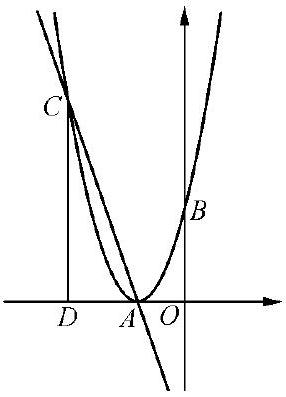
\includegraphics[max width=\textwidth, center]{2024_10_30_1bf34f7aeb61f11d11d3g-099}

图7-4

\begin{align*}
\begin{aligned}
S_{\triangle A B C} & =S_{\text {梯形 } B C D O}-S_{\triangle A C D}-S_{\triangle A B O} \\
& =\frac{1}{2}(4+9) \times 5-\frac{1}{2} \times 3 \times 9-\frac{1}{2} \times 2 \times 4=15 .
\end{aligned}
\end{align*}

例10 如图 7-5 所示,在平面直角坐标系中,矩形 $A B O C$ 的边 $B O$ 在 $x$轴的负半轴上, 边 $O C$ 在 $y$ 轴的正半轴上, 且 $A B=1, O B=\sqrt{3}$, 矩形 $A B O C$绕点 $O$ 按顺时针方向旋转 $60^{\circ}$ 后得到矩形 $E F O D$ 。点 $A$ 的对应点为点 $E$, 点 $B$的对应点为点 $F$, 点 $C$ 的对应点为点 $D$, 抛物线 $y=a x^{2}+b x+c$ 过点 $A 、 E 、 D$.\\
(1)判断点 $E$ 是否在 $y$ 轴上,并说明理由;\\
(2)求抛物线的函数表达式;\\
(3)在 $x$ 轴的上方是否存在点 $P$ 、点 $Q$ ,使以点 $O 、 B 、 P 、 Q$ 为顶点的平行四边形的面积是矩形 $A B O C$ 面积的 2 倍,且点 $P$ 在抛物线上,若存在,请求出点 $P$ 、点 $Q$ 的坐标;若不存在,请说明\\
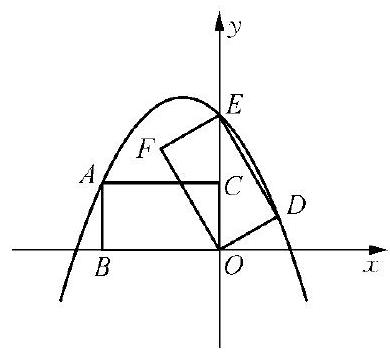
\includegraphics[max width=\textwidth, center]{2024_10_30_1bf34f7aeb61f11d11d3g-099(1)}

图7-5

理由。\\
解 (1)点 $E$ 在 $y$ 轴上,理由如下:\\
连结 $A O$, 如图 $7-6$ 所示, 在 Rt $\triangle A B O$ 中,因为 $A B=1, B O=\sqrt{3}$, 所以 $A O=2$.

从而 $\sin \angle A O B=\frac{1}{2}$, 则 $\angle A O B=30^{\circ}$.\\
由题意可知: $\angle A O E=60^{\circ}$, 所以 $\angle B O E=$ $\angle A O B+\angle A O E=30^{\circ}+60^{\circ}=90^{\circ}$.

因为点 $B$ 在 $x$ 轴上, 故点 $E$ 在 $y$ 轴上.\\
(2)过点 $D$ 作 $D M \perp x$ 轴于点 $M$ 。\\
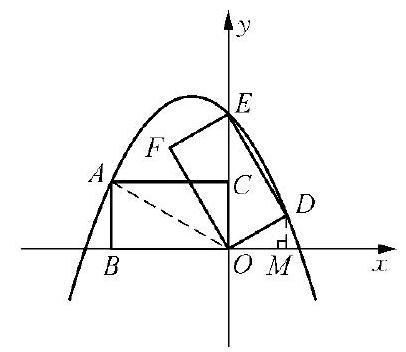
\includegraphics[max width=\textwidth, center]{2024_10_30_1bf34f7aeb61f11d11d3g-100}

图 $7-6$

因为 $O D=1, \angle D O M=30^{\circ}$, 所以在 Rt $\triangle D O M$ 中, $D M=\frac{1}{2}$, $O M=\frac{\sqrt{3}}{2}$.

又因为点 $D$ 在第一象限, 故点 $D$ 的坐标为 $\left(\frac{\sqrt{3}}{2}, \frac{1}{2}\right)$.\\
由 (1) 知 $E O=A O=2$, 点 $E$ 在 $y$ 轴的正半轴上, 所以点 $E$ 的坐标为 $(0$, $2)$, 点 $A$ 的坐标为 $(-\sqrt{3}, 1)$.

又因为抛物线 $y=a x^{2}+b x+c$ 经过点 $E$, 所以 $c=2$.\\
由题意,将 $A(-\sqrt{3}, 1), D\left(\frac{\sqrt{3}}{2}, \frac{1}{2}\right)$ 代入 $y=a x^{2}+b x+2$ 中得

\begin{align*}
\begin{aligned}
& \left\{\begin{array}{l}
3 a-\sqrt{3} b+2=1, \\
\frac{3}{4} a+\frac{\sqrt{3}}{2} b+2=\frac{1}{2},
\end{array}\right. \\
& \left\{\begin{array}{l}
a=-\frac{8}{9}, \\
b=-\frac{5 \sqrt{3}}{9} .
\end{array}\right.
\end{aligned}
\end{align*}

故所求抛物线表达式为 $y=-\frac{8}{9} x^{2}-\frac{5 \sqrt{3}}{9} x+2$.\\
(3) 矩形 $A B O C$ 的面积 $=A B \cdot B O=\sqrt{3}$, 则以 $O 、 B 、 P 、 Q$ 为顶点的平行四边形面积为 $2 \sqrt{3}$ ,由题意可知 $O B$ 为此平行四边形一边。

又因为 $O B=\sqrt{3}$, 所以 $O B$ 边上的高为 2 , 依题意设点 $P$ 的坐标为 (m,2)。

因为点 $P$ 在抛物线 $y=-\frac{8}{9} x^{2}-\frac{5 \sqrt{3}}{9} x+2$ 上,则

解得

\begin{align*}
\begin{gathered}
-\frac{8}{9} m^{2}-\frac{5 \sqrt{3}}{9} m+2=2, \\
m_{1}=0, m_{2}=-\frac{5}{8} \sqrt{3}, \\
P_{1}(0,2) 、 P_{2}\left(-\frac{5}{8} \sqrt{3}, 2\right) .
\end{gathered}
\end{align*}

所以\\
因为以 $O 、 B 、 P 、 Q$ 为顶点的四边形是平行四边形, 所以 $P Q / / O B$, $P Q=O B=\sqrt{3}$, 则当点 $P_{1}$ 的坐标为 $(0,2)$ 时, 点 $Q$ 的坐标分别为 $Q_{1}(-\sqrt{3}$, 2)、 $Q_{2}(\sqrt{3}, 2)$;

当点 $P_{2}$ 的坐标为 $\left(-\frac{5 \sqrt{3}}{8}, 2\right)$ 时, 点 $Q$ 的坐标分别为 $Q_{3}\left(-\frac{13 \sqrt{3}}{8}, 2\right)$ 、 $Q_{4}\left(\frac{3 \sqrt{3}}{8}, 2\right)$.

例11 设 $\overline{a b c}$ 是十进制中的素数,证明: $b^{2}-4 a c$ 不是完全平方数。\\
证明 我们采用反证法.\\
假设存在一个十进制的素数 $\overline{a b c}$ ,使得 $b^{2}-4 a c$ 为完全平方数,注意到求证结果的形式,我们考虑构造二次函数 $f(x)=a x^{2}+b x+c$, 则已知的十进制中的素数

\begin{align*}
p=f(10)=a \times 10^{2}+b \times 10+c=\overline{a b c} .
\end{align*}

由于 $b^{2}-4 a c$ 是一个完全平方数, 故 $f(x)=0$ 的两个根 $x_{1,2}=$ $\frac{-b \pm \sqrt{b^{2}-4 a c}}{2 a}$ 均为有理数, 且 $x_{1} 、 x_{2}$ 都小于 0 , 故 $2 a x_{1} 、 2 a x_{2}$ 为小于 0 的整数.

则有

\begin{align*}
a x^{2}+b x+c=a\left(x-x_{1}\right)\left(x-x_{2}\right),
\end{align*}

令 $x=10$ 得

\begin{align*}
p=a\left(10-x_{1}\right)\left(10-x_{2}\right),
\end{align*}

由于 $2 a x_{1} 、 2 a x_{2}$ 为整数, 两边同乘以 $4 a$ ,得

\begin{align*}
4 a p=\left(20 a-2 a x_{1}\right)\left(20 a-2 a x_{2}\right)
\end{align*}

因为 $p$ 为素数, 所以上面两个式子中必有一个被 $p$ 整除, 不妨设 $20 a-$ $2 a x_{1}$ 是 $p$ 的倍数, 所以 $20 a-2 a x_{1} \geqslant p$, 则 $20 a-2 a x_{2} \leqslant 4 a$, 即 $x_{2} \geqslant 8$, 这与\\
$x_{2}$ 小于 0 矛盾.\\
所以 $b^{2}-4 a c$ 不是完全平方数.\\
评注 当题目中的条件出现形如 $b^{2}-4 a c$ 这一类平方与积的差的形式的式子时,常常利用判别式来构造方程或函数.

例12 求证: $\frac{(x+a)(x+b)}{(c-a)(c-b)}+\frac{(x+b)(x+c)}{(a-b)(a-c)}+\frac{(x+c)(x+a)}{(b-c)(b-a)}=1$.\\
分析 如果把左边的式子通分化简,不但计算量大,且容易出错,但依据要证等式左边的特点, 将 "左边一右边"看成一个关于 $x$ 的二次函数, 则可化繁为简。

证明 构造函数

\begin{align*}
f(x)=\frac{(x+a)(x+b)}{(c-a)(c-b)}+\frac{(x+b)(x+c)}{(a-b)(a-c)}+\frac{(x+c)(x+a)}{(b-c)(b-a)}-1,
\end{align*}

则

\begin{align*}
\begin{aligned}
f(-a)= & \frac{(-a+a)(-a+b)}{(c-a)(c-b)}+\frac{(-a+b)(-a+c)}{(a-b)(a-c)}+ \\
& \frac{(-a+c)(-a+a)}{(b-c)(b-a)}-1 \\
= & \frac{(-a+b)(-a+c)}{(a-b)(a-c)}-1=0,
\end{aligned}
\end{align*}

根据对称性得

\begin{align*}
f(-a)=f(-b)=f(-c)=0
\end{align*}

又 $a \neq b \neq c$, 则二次函数的图象与 $x$ 轴有 3 个不同的交点, 则说明函数 $f(x)$ 恒等于 0 ,故所证的等式成立。

例13 设 $x 、 y 、 z$ 介于 0 与 1 之间, 求证: $x(1-y)+y(1-z)+z(1-$ $x)<1$ 。

分析 我们将要证的关系式中的 $y, z$ 看做常量, 把 $x$ 看做变量, 则待证的关系式就是一个关于 $x$ 的不等式,于是可借助一次函数的图象特征来解决。

证明 构造函数

\begin{align*}
\begin{aligned}
f(x) & =1-[x(1-y)+y(1-z)+z(1-x)] \\
& =(z+y-1) x+(y z+1-y-z),
\end{aligned}
\end{align*}

因为 $0<x 、 y 、 z<1$, 则

\begin{align*}
\begin{aligned}
& f(0)=y z+1-y-z=(y-1)(z-1)>0 \\
& f(1)=(z+y-1)+(y z+1-y-z)=y z>0 .
\end{aligned}
\end{align*}

由于一次函数的图象是一条直线,所以当 $0<x<1$ 时,恒有 $f(x)>0$ 成立,故不等式成立。

例14 已知实数 $x_{1} 、 x_{2}$ 满足 $x_{1}\left(x_{1}+1\right)=1, x_{2}\left(x_{2}+1\right)=1, \frac{x_{1}^{3}}{x_{2}^{3}}+\frac{x_{2}^{3}}{x_{1}^{3}}=$ $m$ ,当 $-2 \leqslant x \leqslant 1$ 时,函数 $f(x)=\frac{m-2}{20} x^{2}+2 n x-4 n \leqslant 0$ 恒成立,求常数 $n$ 的取值范围。

解 (1)当 $x_{1}=x_{2}$ 时, $m=\frac{x_{1}^{3}}{x_{2}^{3}}+\frac{x_{2}^{3}}{x_{1}^{3}}=2$ ,函数为 $f(x)=2 n x-4 n$ 。\\
要使当 $-2 \leqslant x \leqslant 1$ 时,函数 $f(x) \leqslant 0$ 恒成立,只需

\begin{align*}
\left\{\begin{array}{l}
f(-2) \leqslant 0, \\
f(1) \leqslant 0,
\end{array}\right.
\end{align*}

解得

\begin{align*}
n \geqslant 0
\end{align*}

故当 $x_{1}=x_{2}$ 时, $n$ 的取值范围是 $n \geqslant 0$.\\
(2)当 $x_{1} \neq x_{2}$ 时,由题意得 $x_{1} 、 x_{2}$ 是方程 $t^{2}+t-1=0$ 的两个根。\\
由韦达定理得 $x_{1}+x_{2}=-1, x_{1} \cdot x_{2}=-1$ ,于是 $m=\frac{x_{1}^{3}}{x_{2}^{3}}+\frac{x_{2}^{3}}{x_{1}^{3}}=\frac{x_{1}^{6}+x_{2}^{6}}{x_{1}^{3} \cdot x_{2}^{3}}=-\left(x_{1}^{6}+x_{2}^{6}\right)=-\left(x_{1}^{2}+x_{2}^{2}\right)\left[\left(x_{1}^{2}+x_{2}^{2}\right)^{2}-3 x_{1}^{2} x_{2}^{2}\right]$.

而 $x_{1}^{2}+x_{2}^{2}=\left(x_{1}+x_{2}\right)^{2}-2 x_{1} x_{2}=3$, 则代入上式得 $m=-18$.\\
此时函数 $f(x)=-x^{2}+2 n x-4 n=-(x-n)^{2}+n^{2}-4 n$ ,当 $-2 \leqslant x \leqslant$ 1 时, $f(x) \leqslant 0$ 恒成立. 可分三种情况考虑:\\
(1) 当 $n<-2$ 时, 只需 $f(-2) \leqslant 0$, 即 $-4-4 n-4 n \leqslant 0 \Rightarrow n \geqslant-\frac{1}{2}$, 这与 $n<-2$ 矛盾,舍去;\\
(2) 当 $-2 \leqslant n \leqslant 1$ 时, 只需 $n^{2}-4 n \leqslant 0 \Rightarrow 0 \leqslant n \leqslant 4$, 故 $n$ 的取值范围为 $0 \leqslant n \leqslant 1$ ;\\
(3) 当 $n>1$ 时, 只需 $f(1) \leqslant 0$, 即 $-1+2 n-4 n \leqslant 0 \Rightarrow n \geqslant-\frac{1}{2}$, 故 $n$ 的取值范围为 $n>1$ 。

由以上三种情况知,当 $x_{1} \neq x_{2}$ 时, $n$ 的取值范围为 $n \geqslant 0$ 。\\
综合(1)(2)得 $n$ 的取值范围为 $n \geqslant 0$ 。\\
例 15 两辆汽车从同一地点同时出发,沿同一方向以相等的速度直线行驶,每车最多只能带 24 桶汽油,途中不能用别的汽油,每桶油可使一辆汽车前进 60 km ,两车必须返回出发地点,但是可以不同时返回,也可以两车相互借用对方的汽油,为了使其中一辆车尽可能地远离出发点,另一辆车应当在离出发点多少千米的地方返回? 离出发点远的那辆车一共行驶了多少千米?

解 设两辆车分别为甲、乙,并且甲用了 $x$ 桶汽油时返回,留下返程需要的 $x$ 桶汽油,将多余的 $(24-2 x)$ 桶汽油给乙,让乙继续前进。

这时乙有 $(24-2 x)+(24-x)=48-3 x$ 桶汽油, 又因为每车最多只能带 24 桶汽油,则有

\begin{align*}
48-3 x \leqslant 24 \Rightarrow x \geqslant 8
\end{align*}

甲、乙分手后,乙继续前进的路程是 $\frac{(48-3 x)-x}{2} \times 60=30(48-4 x)$.\\
考查函数 $y=30(48-4 x), y$ 随着 $x$ 的增大而减少,所以当 $x=8$ 时,有最大值 480 km , 因此甲应该在离出发点 480 km 时返回, 乙行驶的路程一共为 $2(480+60 \times 8)=1920(k m)$.\\
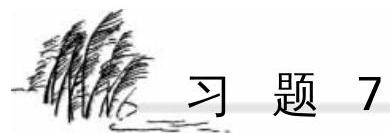
\includegraphics[max width=\textwidth, center]{2024_10_30_1bf34f7aeb61f11d11d3g-104}

1 关于 $x 、 y$ 的方程 $x^{2}+x y+2 y^{2}=29$ 的整数解 $(x, y)$ 有 ( ) 组.\\
A. 2\\
B. 3\\
C. 4\\
D. 5

2 已知对所有实数 $x,|x+1|+\sqrt{x-1} \geqslant m-|x-2|$ 恒成立, 则 $m$ 可取得的最大值为 $\qquad$ .\\
3 设点 $A 、 B$ 是抛物线 $y=2 x^{2}+4 x-2$ 上的点, 原点位于线段 $A B$ 的中点处, 试求 $A 、 B$ 两点的坐标。\\
4 设 $m 、 n$ 为正整数, 且 $m \neq 2$, 如果对一切实数 $t$, 二次函数 $y=x^{2}+(3-$ $m t) x-3 m t$ 的图象与 $x$ 轴的两个交点间的距离不小于 $|2 t+n|$, 求 $m 、 n$的值。\\
5 求方程 $[2 x]+[3 x]=9 x-\frac{7}{4}$ 的所有实数解.\\
6 求满足 $25\{x\}+[x]=125$ 的所有实数 $x$ 的和(其中 $\{x\}$ 表示 $x$ 的小数部分).

7 若反比例函数 $y=\frac{k}{x}$ 的图象与一次函数 $y=a x+b$ 的图象交于点 $A(-2, m) 、 B(5, n)$, 求 $3 a+b$ 的值.\\
8 已知二次函数 $y=x^{2}-x+a$ 的图象与 $x$ 轴的两个不同的交点到原点的距离之和不超过 5 ,求 $a$ 的取值范围。\\
9 在直角坐标系 $x O y$ 中,一次函数 $y=k x+b(k \neq 0)$ 的图象与 $x$ 轴、 $y$ 轴的正半轴分别交于点 $A 、 B$, 且使得 $\triangle O A B$ 的面积值等于 $|O A|+|O B|+3$.\\
(1)用 $b$ 表示 $k$;\\
(2)求 $\triangle O A B$ 面积的最小值.\\
10 已知一次函数 $y_{1}=2 x$ ,二次函数 $y_{2}=x^{2}+1$ ,是否存在二次函数 $y_{3}=$ $a x^{2}+b x+c$ ,其图象经过点 $(-5,2)$ ,且对于任意一个实数 $x$ ,这三个函数所对应的函数值 $y_{1} 、 y_{2} 、 y_{3}$ ,都有 $y_{1} \leqslant y_{3} \leqslant y_{2}$ 成立?若存在,求出函数 $y_{3}$ 的解析式;若不存在,请说明理由。\\
11 已知点 $A 、 B$ 分别在一次函数 $y=x, y=8 x$ 的图象上, 其横坐标分别为 $a 、 b(a>0, b>0)$ ,若直线 $A B$ 为一次函数 $y=k x+m$ 的图象,则当 $\frac{b}{a}$是整数时,求满足条件的整数 $k$ 的值。\\
12 一幢 33 层的大楼有一部电梯停在第一层,它一次最多容纳 32 人,而且只能在第2层至第33层中某一层停一次,对于每个人来说,他往下走一层楼梯感到 1 分不满意,往上走一层楼梯感到 3 分不满意,现在有 32 个人在第一层,并且他们分别住在第2至第33层的每一层,问:电梯停在哪一层时,可以使得这 32 个人不满意的总分达到最小?最小值是多少?(有些人可以不乘电梯即直接从楼梯上楼)。\\
13 有 20 条输入传送带, 20 条输出传送带。控制室的电脑显示,每条输入传送带每小时进库的货物流量如图(1),每条输出传送带每小时出库的货物流量如图(2),而该日仓库中原有货物 8 吨,在 0 时至 5 时,仓库中货物存量变化情况如图(3),则在 0 时至 2 时有多少条输入传送带和输出传送带在工作,在 4 时至 5 时有多少条输入传送带和输出传送带在工作?\\
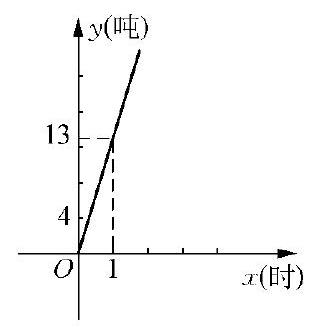
\includegraphics[max width=\textwidth, center]{2024_10_30_1bf34f7aeb61f11d11d3g-105}

图(1)\\
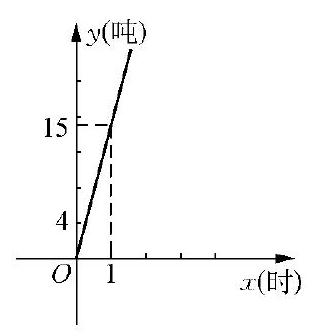
\includegraphics[max width=\textwidth, center]{2024_10_30_1bf34f7aeb61f11d11d3g-105(1)}

图(2)\\
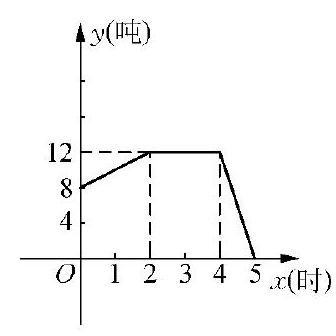
\includegraphics[max width=\textwidth, center]{2024_10_30_1bf34f7aeb61f11d11d3g-105(2)}

图(3)

14 在平面直角坐标系中,直线 $y=-\sqrt{3} x-\sqrt{3}$ 与 $x$ 轴交于点 $A$ ,与 $y$ 轴交于点 $C$ ,拖物线 $y=a x^{2}-\frac{2 \sqrt{3}}{3} x+c(a \neq 0)$ 经过 $A 、 B 、 C$ 三点。\\
(1)求过 $A 、 B 、 C$ 三点抛物线的解析式并求出顶点 $F$ 的坐标;\\
(2)在抛物线上是否存在点 $P$, 使 $\triangle A B P$ 为直角三角形, 若存在, 直接写

出 $P$ 点坐标;若不存在,请说明理由;\\
(3)试探究在直线 $A C$ 上是否存在一点 $M$ ,使得 $\triangle M B F$ 的周长最小,若存在,求出 $M$ 点的坐标;若不存在,请说明理由。\\
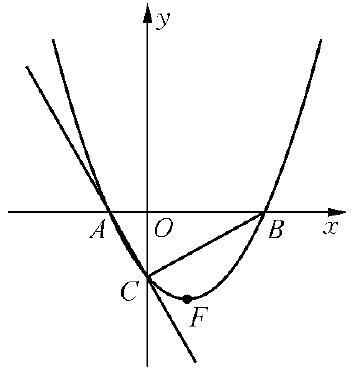
\includegraphics[max width=\textwidth, center]{2024_10_30_1bf34f7aeb61f11d11d3g-106}\\
(第 14 题)\\
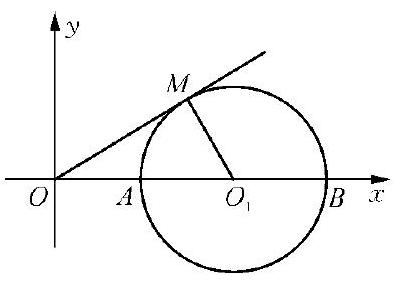
\includegraphics[max width=\textwidth, center]{2024_10_30_1bf34f7aeb61f11d11d3g-106(1)}\\
(第 15 题)

15 如图,已知半径为 1 的 $\odot O_{1}$ 与 $x$ 轴交于 $A 、 B$ 两点, $O M$ 为 $\odot O_{1}$ 的切线,切点为 $M$ ,圆心 $O_{1}$ 的坐标为 $(2,0)$ ,二次函数 $y=-x^{2}+b x+c$ 的图象经过 $A 、 B$ 两点。\\
(1)求二次函数的解析式;\\
(2)求切线 $O M$ 的函数解析式;\\
(3)线段 $O M$ 上是否存在一点 $P$ ,使得以 $P 、 O 、 A$ 为顶点的三角形与 $\triangle O O_{1} M$ 相似. 若存在, 请求出所有符合条件的点 $P$ 的坐标; 若不存在,请说明理由。

\section*{习题解答}
\section*{习 题 1}
\begin{enumerate}
  \item 如图, 满足已知条件的 6 条直线至多有 10 个交点,增加一条直线与这 6 条直线最多有 6 个交点,再增加一条直线与前 7 条直线最多有 7 个交点 $\cdots$ —直增加到第 10 条直线与前 9条直线最多有 9 个交点,所以这 10 条直线的交点个数最多有: $10+6+7+8+9=40$ (个), 故选 B.
  \item 由题意,矩形 $O A P B$ 的面积为 $S=$\\
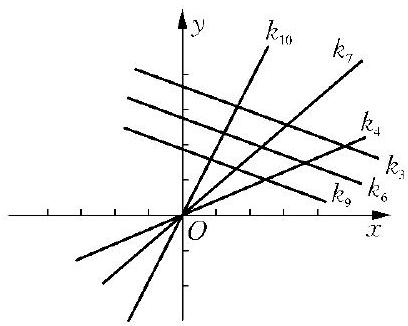
\includegraphics[max width=\textwidth, center]{2024_10_30_1bf34f7aeb61f11d11d3g-107}\\
(第 1 题)\\
$|P A| \times|P B|$, 设 $P$ 点坐标为 $P\left(x_{P},-x_{P}+3\right)$, 则 $|P A|=\left|y_{P}\right|=\mid-x_{P}+$ $3\left|,|P B|=\left|x_{P}\right|\right.$ ,得到 $\left.S=\left|x_{P}\right|\right|-x_{P}+3 \mid=2$ ,即 $x_{P}^{2}-3 x_{P}-2=0$ 或 $x_{P}^{2}-3 x_{P}+2=0$ ,解得 $x_{P}=\frac{3-\sqrt{17}}{2} , x_{P}=\frac{3+\sqrt{17}}{2} , x_{P}=1, x_{P}=2$ 。所以关于 $P$ 的横坐标 $x_{P}$ 的方程有 4 个不同的解, 所求 $P$ 点一共有四个, 坐标为 $\left(\frac{3-\sqrt{17}}{2}, \frac{3+\sqrt{17}}{2}\right),\left(\frac{3+\sqrt{17}}{2}, \frac{3-\sqrt{17}}{2}\right),(1,2),(2,1)$.
  \item 因为 $2 x+y=6$, 得 $y=6-2 x$, 代入 $x+3 y+|3 x-y|=19$ 中, 有 $x+3(6-2 x)+|3 x-(6-2 x)|=19$, 整理为 $|5 x-6|=5 x+1$. 又因为 $5 x-6<5 x+1$, 所以 $-(5 x-6)=5 x+1$, 解得 $x=\frac{1}{2}, y=5$.
  \item 由题意 $|a|=a+1$, 得 $a=-\frac{1}{2}$, 代入 $|x|=2 a x$, 得 $x \leqslant 0$, 则有 $|x-1|-|x+1|+2=3-x-|x+1|$ 。当 $-1 \leqslant x \leqslant 0$ 时, 原式 $=3-$ $x-(x+1)=2-2 x$ ,最大值为 4 ,最小值为 2 ;当 $x<-1$ 时,原式 $=3-x+$ $(x+1)=4$ 。所以最大值为 4 , 最小值为 2 .
  \item 根据题意 $S_{\triangle O A D}=S_{\triangle O B C}=\frac{15}{2}$, 并且 $S_{\triangle A E C}=S_{\triangle E D B}, S_{\triangle O E C}=S_{\triangle O E D}$.
\end{enumerate}

设 $S_{\triangle A E C}=x, S_{\triangle O E C}=y$, 则 $\frac{x}{y}=\frac{2}{3} \Rightarrow 2 y=3 x$, 又 $x+2 y=\frac{15}{2}$ ,解得 $x=\frac{15}{8}$ ,则 $S_{\triangle A E B}=S_{\triangle A B C}-$ $S_{\triangle A C E}=5-\frac{15}{8}=\frac{25}{8}$.\\
6. 由题意要使 $y=\frac{1}{3} x+b$ 的图象将矩形\\
\includegraphics[max width=\textwidth, center]{2024_10_30_1bf34f7aeb61f11d11d3g-108}\\
(第 5 题)\\
$O A B C$ 分成面积相等的两部分, 由于 $O A B C$ 是中心对称图形。所以 $y=\frac{1}{3} x+b$ 必过 $O A B C$ 的中心 $G$ 点,而由于 $B$ 的坐标为( 15 , 6), $G$ 是 $O A B C$ 的中心, 易得 $G$ 的横、纵坐标都是 $B$ 的横、纵坐标的一半, 得 $G\left(\frac{15}{2}, 3\right)$. 所以代入直线方程 $y=\frac{1}{3} x+b$, 有 $3=\frac{1}{3} \times \frac{15}{2}+b$, 得 $b=\frac{1}{2}$.\\
7. (1) 函数 $y=x+1$ 与 $y=2 x$ 的生成函数为 $y=m(x+1)+n(2 x)$,则当 $x=1$ 时,其函数值为 $y=2 m+2 n=2(m+n)=2$ 。\\
(2) 设点 $P$ 的坐标为 $(a, b)$, 则有 $a_{1} a+b_{1}=b, a_{2} a+b_{2}=b$. 两个函数生成的函数为: $y=m\left(a_{1} x+b_{1}\right)+n\left(a_{2} x+b_{2}\right)$ ,当 $x=a$ 时,有 $y=m\left(a_{1} a+\right.$ $\left.b_{1}\right)+n\left(a_{2} a+b_{2}\right)=m b+n b=b(m+n)=b$ ,即点 $P$ 在此两个函数的生成函数的图象上。\\
8. 由题意, 设 $O P=l(0<l<7), P C=7-l$, 由 $P A \perp P B$, 得 Rt $\triangle P B C \backsim$ $\mathrm{Rt} \triangle A O P$ ,有 $\frac{3}{l}=\frac{7-l}{2}$ ,得 $l^{2}-7 l+6=0$ ,有 $l=1$ 或 $l=6$ 。当 $l=1$ 时,由 $P(0,1) 、 A(3,0) 、 B(2,7)$ ,可得 $y_{1}=3 x+1, y_{2}=-\frac{1}{3} x+1$ ;当 $l=6$ 时,由 $P(0,6) 、 A(3,0) 、 B(2,7)$, 可得 $y_{1}=\frac{1}{2} x+6, y_{2}=-2 x+6$. 所以当 $l=1$ 时, 有 $k_{1}=3, k_{2}=-\frac{1}{3}, k_{1} k_{2}\left(k_{1}+k_{2}\right)=3 \times\left(-\frac{1}{3}\right)\left[3+\left(-\frac{1}{3}\right)\right]=$ $-\frac{8}{3}$; 当 $l=6$ 时, 有 $k_{1}=\frac{1}{2}, k_{2}=-2, k_{1} k_{2}\left(k_{1}+k_{2}\right)=\frac{1}{2} \times(-2)\left[\frac{1}{2}+\right.$ $(-2)]=\frac{3}{2}$. 综合可得 $k_{1} k_{2}\left(k_{1}+k_{2}\right)$ 的值为 $-\frac{8}{3}$ 或 $\frac{3}{2}$.\\
9. 设 $P^{\prime}$ 为 $P$ 关于 $x$ 轴的对称点, 由 $P(2,1)$ 可得 $P^{\prime}(2,-1)$, 由于 $P$ 与 $P^{\prime}$ 关于 $x$ 轴对称,当 $M$ 在 $x$ 轴上运动时,始终有 $P^{\prime} M=P M$ 。所以, $P M+$ $M Q=P^{\prime} M+M Q \geqslant P^{\prime} Q$ 。设 $P^{\prime} Q$ 与 $x$ 轴的交点为 $N$, 当点 $M$ 与 $N$ 重合时, $P M+M Q$ 取最小值. 由条件 $P^{\prime}(2,-1), Q(5,5)$ ,可得过 $P^{\prime} 、 Q$ 的一次函数

的图象 (直线) 的解析式为 $y=2 x-5$. 当 $y=0$ 时, $x=\frac{5}{2}$, 即当 $M$ 的坐标为 $M\left(\frac{5}{2}, 0\right)$ 时 $P M+M Q$ 的值最小.\\
10. 如图, 设 $A$ 点关于 $x$ 轴的对称点为 $A^{\prime}$, 即 $A^{\prime}(-8,-3) . B$ 点关于 $y$轴的对称点为 $B^{\prime}(4,5)$, 则 $A D=A^{\prime} D, B C=B^{\prime} C$, 得 $l=B A+A D+D C+$ $C B=B A+A^{\prime} D+D C+C B^{\prime} \geqslant A^{\prime} B^{\prime}+B A$ 。当 $D 、 C 、 A^{\prime} 、 B^{\prime}$ 四点共线, 即 $C$ 、 $D$ 分别是 $A^{\prime} B^{\prime}$ 与 $y$ 轴、 $x$ 轴的交点时, $l$ 取最小值,此时由 $A^{\prime}(-8,-3), B^{\prime}(4,5)$ ,可求得直线 $A^{\prime} B^{\prime}$的函数解析式为 $y=\frac{2}{3} x+\frac{7}{3}$. 当 $x=0$ 时, $y=\frac{7}{3}$ ;当 $y=0$ 时, $x=-\frac{7}{2}$. 得 $D\left(-\frac{7}{2}, 0\right), C\left(0, \frac{7}{3}\right)$,即此时 $m=-\frac{7}{2}, n=\frac{7}{3}$, 所以 $m: n=\left(-\frac{7}{2}\right)$ : $\frac{7}{3}=-\frac{3}{2}$.\\
\includegraphics[max width=\textwidth, center]{2024_10_30_1bf34f7aeb61f11d11d3g-109(1)}\\
(第 10 题)\\
11. 如图, 作 $A D \perp x$ 轴于 $D$ 点, $B E \perp x$ 轴于 $E$点, $A F \perp B E$ 于 $F$ 点, 则易得 $\triangle A F B \cong \triangle A D O$ ,而 $\angle A O D=30^{\circ}, O A=1$, 有 $A D=\frac{1}{2}, O D=\frac{\sqrt{3}}{2}$, 所以 $O E=O D-E D=O D-A F=O D-A D=\frac{\sqrt{3}}{2}-$ $\frac{1}{2}, B E=B F+F E=O D+A D=\frac{\sqrt{3}}{2}+\frac{1}{2}$. 所以 $B$点坐标为 $\left(\frac{\sqrt{3}-1}{2}, \frac{\sqrt{3}+1}{2}\right)$.\\
\includegraphics[max width=\textwidth, center]{2024_10_30_1bf34f7aeb61f11d11d3g-109}\\
(第 11 题)\\
12. (1)总运费为 $w=400 \times(10-x)+800 \times[8-(6-x)]+300 x+$ $500(6-x)=200 x+8600$ 。由于 $10-x \geqslant 0,8-(6-x) \geqslant 0, x \geqslant 0,6-$ $x \geqslant 0$, 可得 $0 \leqslant x \leqslant 6$ ( $x$ 为整数)。所以 $w=200 x+8600(0 \leqslant x \leqslant 6, x$ 为整数)。\\
(2)由题意得 $w \leqslant 9000$ ,即 $200 x+8600 \leqslant 9000$ ,解得 $0 \leqslant x \leqslant 2(x$ 为整数)。所以 $x$ 可取 $0 、 1 、 2$ ,有三种取法,相对应就有三种调运方案。\\
(3)由于 $w=200 x+8600(~ 0 \leqslant x \leqslant 6, x$ 为整数),易得当 $x=0$ 时,总费用最低,即从 $B$ 市运 6 台到 $D$ 市,以 $A$ 市运 10 台到 $C$ 市、运 2 台到 $D$ 市,最低费用 8600 元。\\
13. (1)由于直线 $y=-k x+b(k>0)$ 与 $y=\frac{5}{x}$ 交于 $C$ 点 $(1,5)$, 有 $5=-k+b$, 即 $b=5+k$. 所以 $y=-k x+b=-k x+5+k$ 。而 $A$ 点是直线与 $x$ 轴的交点,当 $y=0$ 时,有 $x=\frac{5+k}{k}(k>0)$ ,即得 $A\left(\frac{5+k}{k}, 0\right)$ ,从而 $a=$ $\frac{5+k}{k}(k>0)$.\\
(2)若直线与 $y=\frac{5}{x}$ 在第一象限的另一交点 $D$ 的横坐标 $x=9$ 时, 而 $D$在 $y=\frac{5}{x}$ 上, 由 $y=\frac{5}{x}, x=9$, 得 $y=\frac{5}{9}$, 即得 $D\left(9, \frac{5}{9}\right)$. 又 $y=-k x+b=$ $-k x+5+k$, 所以 $\frac{5}{9}=-k \times 9+5+k$, 得 $k=\frac{5}{9}$, 从而 $a=\frac{5+k}{k}=\frac{5}{k}+1=$ $\frac{9}{5} \times 5+1=10$. 作 $C E \perp x$ 轴于 $E$ 点, 则 $C E=5$, 得 $S_{\triangle C O A}=\frac{1}{2} \times O A \times C E=$ $\frac{1}{2} \times 10 \times 5=25$.\\
14. (1) 因为直线 $y=k_{1} x+b$, 过点 $(1,6)$和 $(-3,-2)$ ,有 $\left\{\begin{array}{l}6=k_{1}+b_{1}, \\ -2=-3 k_{1}+b_{1}\end{array}\right.$ ,解得 $\left\{\begin{array}{l}k_{1}=2, \\ b_{1}=4,\end{array}\right.$ 所以 $y=2 x+4$. 直线 $y=k_{2} x+b_{2}$ 过点 $(2,-2)$, 且在 $y$ 轴上的截距为 -3 , 有 $\left\{\begin{array}{l}-3=k_{2} \times 0+b_{2}, \\ -2=2 \times k_{2}+b_{2}\end{array}\right.$, 得 $\left\{\begin{array}{l}b_{2}=-3, \\ k_{2}=\frac{1}{2},\end{array}\right.$ 所以 $y=$\\
\includegraphics[max width=\textwidth, center]{2024_10_30_1bf34f7aeb61f11d11d3g-110}\\
(第 14 题)\\
$\frac{1}{2} x-3$. 两条直线的图象如图所示.\\
(2) 直线 $y=2 x+4$ 与 $y$ 轴、 $x$ 轴分别交于点 $A(0,4) 、 B(-2,0)$. 直线 $y=\frac{1}{2} x-3$ 与 $y$ 轴、 $x$ 轴分别交于点 $C(0,-3) 、 D(6,0)$, 所以 $S_{\text {四边形 } A B C D}=$ $S_{\triangle A B D}+S_{\triangle B D C}=\frac{1}{2} B D \times A O+\frac{1}{2} B D \times C O=\frac{1}{2} \times 8 \times 4+\frac{1}{2} \times 8 \times 3=$ $16+12=28$.\\
(3)由 $\left\{\begin{array}{l}y=2 x+4, \\ y=\frac{1}{2} x-3,\end{array}\right.$ 解得 $\left\{\begin{array}{l}x=-\frac{14}{3}, \\ y=-\frac{16}{3},\end{array}\right.$ 即 $E$ 的坐标为 $\left(-\frac{14}{3},-\frac{16}{3}\right)$. 过点\\
$E$ 作 $E F \perp y$ 轴于点 $F$, 则有 $S_{\triangle A D E}=S_{\triangle A C E}+S_{\triangle A C D}=\frac{1}{2} \times A C \times E F+\frac{1}{2} A C \times$ $O D=\frac{1}{2} \times 7 \times \frac{14}{3}+\frac{1}{2} \times 7 \times 6=\frac{112}{3}, S_{\triangle B C E}=S_{\triangle A D E}-S_{\text {四边形 } A B C D}=\frac{112}{3}-$ $28=\frac{28}{3}$, 所以 $S_{\triangle B C E}: S_{\triangle A D E}=\frac{28}{3}: \frac{112}{3}=1: 4$.\\
15. (1)由题意得 $y=m x+4, y$ 随 $x$ 增大而减小,有 $m<0$. 又四边形 $A B C D$ 为凸四边形,则 $D$ 处于 $C$ 点上方。又 $A$ 在第一象限,则 $A$ 的纵坐标大于 0 . 由 $\left\{\begin{array}{l}y=m x+4, \\ x=1,\end{array}\right.$ 和 $\left\{\begin{array}{l}y=m x+4, \\ x=4,\end{array}\right.$ 解得 $A(1, m+4), D(4,4 m+4)$, , 故 $m+$ $4>0,4+4 m>0$, 得 $m>-1$. 所以 $-1<m<0$.\\
(2) 四边形 $A B C D$ 是凸四边形,且 $A B=m+4, C D=4 m+4$. 由 $\frac{E D}{E A}=$ $\frac{4}{7}$, 可得 $\frac{C D}{A B}=\frac{4}{7}, \frac{4 m+4}{m+4}=\frac{4}{7}, m=-\frac{1}{2}$, 所以一次函数解析式为 $y=$ $-\frac{1}{2} x+4$.\\
(3) 由 $y=-\frac{1}{2} x+4$ 可得当 $y=0$ 时, $x=8$, 即得 $E(8,0)$. 由已知得 $C(4$, 0) 则 $C$ 为 $E O$ 中点. 所以 $C D$ 为 Rt $\triangle E O F$ 的中位线, $D$ 即为 $\triangle E O F$ 的外心.

\section*{习 题 2}
\begin{enumerate}
  \item 因为 $x^{2}-100 x+196=(x-2)(x-98)$, 则当 $2 \leqslant x \leqslant 98$ 时, $\mid x^{2}-$ $100 x+196 \mid=-\left(x^{2}-100 x+196\right)$ ,即当自变量 $x$ 取 $2,3,4, \cdots, 98$ 时,函数值都为 0 。而当 $x$ 取值 $1,99,100$ 时, $\left|x^{2}-100 x+196\right|=\left(x^{2}-100 x+\right.$ 196),即 $y=x^{2}-100 x+196=(x-2)(x-98)$ 。故所求的和为 $(1-2)(1-$ $98)+(99-2)(99-98)+(100-2)(100-98)=97+97+196=390$, 选 B.
  \item 设点 $A$ 的坐标为 $\left(a, a^{2}\right)$, 点 $C$ 的坐标为 $\left(c, c^{2}\right),(|c|<|a|)$, 则点 $B$的坐标为 $\left(-a, a^{2}\right)$, 由勾股定理, 得 $A C^{2}=(c-a)^{2}+\left(c^{2}-a^{2}\right)^{2}, B C^{2}=$ $(c+a)^{2}+\left(c^{2}-a^{2}\right)^{2}, A C^{2}+B C^{2}=A B^{2}$ ,所以 $\left(a^{2}-c^{2}\right)^{2}=a^{2}-c^{2}$ 。由于 $a^{2}>$ $c^{2}$ ,所以 $a^{2}-c^{2}=1$ ,根据图象知斜边 $A B$ 上高 $h^{2}=a^{2}-c^{2}=1$ ,所以 $h=1$ ,故选 B.
  \item 由已知 $f(x)=a(x-19)(x-99)+2005, c=19 \times 99 a+2005=$ $1881 a+2005$. 由 $|c|<1000$, 且 $a$ 是整数, $a \neq 0$, 得 $a=-1, c=2005-$ $1881=124$.
  \item 根据图象可知 $a<0$, 又因为经过点 $(1,0)$ 与 $(0,1)$, 所以有\\
$\left\{\begin{array}{l}a+b+c=0, \\ c=1,\end{array}\right.$ 得 $\left\{\begin{array}{l}b=-a-1, \\ c=1 .\end{array}\right.$ 于是 $y=a x^{2}-(a+1) x+1=a\left(x-\frac{a+1}{2 a}\right)^{2}-$ $\frac{(a-1)^{2}}{4 a}$. 再由图象可知 $\left\{\begin{array}{l}\frac{a+1}{2 a}<0, \\ -\frac{(a-1)^{2}}{4 a}>0,\end{array}\right.$ 得 $-1<a<0$.
  \item 设 $A\left(x_{1}, 0\right), B\left(x_{2}, 0\right)$, 由 $\triangle A B C$ 是直角三角形, 可知 $x_{1} 、 x_{2}$ 必定异号,则 $x_{1} x_{2}=\frac{c}{a}<0$ 。由射影定理知 $|O C|^{2}=|A O| \cdot|B O|$ ,即 $c^{2}=\left|x_{1}\right| \cdot$ $\left|x_{2}\right|=\left|\frac{c}{a}\right|$. 故 $|a c|=1$ ,所以 $a c=-1$ 。
  \item 由已知得 $A(4,0) 、 B(-4,0)$, 故设另一抛物线为 $y=a(x-4) \cdot$ $(x+4)$. 又 $\triangle A P B$ 是等腰直角三角形, 则 $P$ 点坐标为 $(0,4)$ 或 $(0,-4)$, 所以可得 $\left\{\begin{array}{l}a=\frac{1}{4}, \\ b=0, \\ c=-4,\end{array}\right.$ 或 $\left\{\begin{array}{l}a=-\frac{1}{4}, \\ b=0, \\ c=4 .\end{array}\right.$
  \item 由 $\left\{\begin{array}{l}y=a x^{2}+b x+c, \\ y=k(x-1)-\frac{k^{2}}{4},\end{array}\right.$ 整理得 $a x^{2}+(b-k) x+\left(c+k+\frac{k^{2}}{4}\right)=0$. 因为只有一个公共点, 故 $\Delta=(b-k)^{2}-4 a\left(c+k+\frac{k^{2}}{4}\right)=0$, 即 $(1-a) k^{2}-$ $2(b+2 a) k+\left(b^{2}-4 a c\right)=0$. 由于上式对任意的实数 $k$ 均成立,即各项系数为 0 ,故解得 $a=1, b=-2, c=1$ 。所求解析式为 $y=x^{2}-2 x+1$ 。
  \item 把 $x=3, y=3$ ,代入二次函数 $y=x^{2}+(a+1) x+b$ ,得 $b=-3 a-$ 9. 当 $x$ 为任意实数时, 都有 $y \geqslant x$ ,即 $x^{2}+(a+1) x+b \geqslant x$ 。把 $b=-3 a-9$,代入得 $x^{2}+a x-3 a-9 \geqslant 0$ ,则 $\Delta=a^{2}-4(-3 a-9)=(a+6)^{2} \leqslant 0$ 。所以 $a=-6$, 得 $b=9$. 因此, 二次函数解析式为 $y=x^{2}-5 x+9$, 顶点为 $P\left(\frac{5}{2}, \frac{11}{4}\right)$ ,所以 $O P=\sqrt{\left(\frac{5}{2}\right)^{2}+\left(\frac{11}{4}\right)^{2}}=\frac{\sqrt{221}}{4}$.
  \item 考虑二次函数 $y=a x^{2}-(b-c) x+(a+b+c)$, 当 $x=0$ 时, $y_{1}=$ $a+b+c$ ;当 $x=1$ 时, $y_{2}=2(a+c)$ 。由 $y_{1} y_{2}<0$ ,推知此函数在 $x=0$ 和 $x=1$ 时函数值异号,即其图象与 $x$ 轴有两个交点。因此,必须有 $\Delta=(b-c)^{2}-$ $4 a(a+b+c)>0$ ,即 $(b-c)^{2}>4 a(a+b+c)$.
  \item 与 $x$ 轴交点的横坐标为 $x_{1} 、 x_{2}$, 故抛物线为 $y=a\left(x-x_{1}\right)\left(x-x_{2}\right)$图象过 $(-1,2)$ ,即有 $2=a\left(1+x_{1}\right)\left(1+x_{2}\right)$ ,解得 $a=\frac{2}{\left(1+x_{1}\right)\left(1+x_{2}\right)}$ ,由
\end{enumerate}

条件得 $-1 \leqslant 1+x_{1}<0,1<1+x_{2} \leqslant 2$ ,所以 $-2 \leqslant\left(1+x_{1}\right)\left(1+x_{2}\right)<$ $0, a$ 为负数. 于是,可得 $a \leqslant-1$ 。\\
11. 由 $A(-1, a) 、 B(2,4 a)$, 得 $O A=\sqrt{a^{2}+1}, O B=\sqrt{4+16 a^{2}}$, $A B=\sqrt{9+9 a^{2}}$. 因为 $a \geqslant 1$ ,故 $O A$ 边最小,即 $O A$ 不可能为斜边。(1)若 $O B$为斜边,则 $O B^{2}=O A^{2}+A B^{2}$ ,即 $4+16 a^{2}=a^{2}+1+9+9 a^{2} , 6 a^{2}=6$ ,即 $a^{2}=1$, 由 $a \geqslant 1$, 得 $a=1 . \triangle A O B$ 周长为 $\sqrt{2}+\sqrt{20}+\sqrt{18}=4 \sqrt{2}+2 \sqrt{5}$.\\
(2)若 $A B$ 为斜边,则 $A B^{2}=O A^{2}+O B^{2}$ ,即 $9+9 a^{2}=a^{2}+1+4+16 a^{2}$, $8 a^{2}=4, a^{2}=\frac{1}{2}$ (不合题意). 所以 $\triangle A O B$ 的周长为 $4 \sqrt{2}+2 \sqrt{5}$.\\
12. 整理抛物线族的解析式,得 $y=2(x-m)^{2}+m+1$ ,顶点 $(m, m+1)$在直线 $y=x+1$ 上, 可知这些抛物线掠过区域是一条直线上方的半平面, 这条直线与这些抛物线都只有一个交点, 设此直线为 $y=x+b$, 由 $\left\{\begin{array}{l}y=2 x^{2}-4 m x+2 m^{2}+m+1, \\ y=x+b,\end{array}\right.$ 得 $2 x^{2}-(4 m+1) x+2 m^{2}+m+1-b=0$,由 $\Delta=0$, 得 $b=\frac{7}{8}$, 即直线为 $y=x+\frac{7}{8}$, 而圆心 $\left(\frac{1}{8}, 1\right)$ 恰好在直线上, 所以相交部分为半圆,面积 $S=\frac{\pi}{2}$.\\
13. 二次方程 $a x^{2}+b x+c=0$ 的根是二次函数 $y=a x^{2}+b x+c$ 图象与 $x$ 轴交点的横坐标。现设 $y_{1}=x^{2}-2 m x+m^{2}-1=(x-m)^{2}-1, y_{2}=x^{2}-$ $2 m x+k=(x-m)^{2}+k-m^{2}$ 。可知问题等价于顶点 $\left(m, k-m^{2}\right)$ 在 $(m,-1)$的下方, 即当 $x=m$ 时, $k-m^{2}<-1$, 所以 $k<m^{2}-1$.\\
14. (1)显然抛物线过原点,与 $x$ 轴另一交点的横坐标为 $-\frac{b}{a}$ 。由题知 $15<-\frac{b}{a}<16$, 即 $-\frac{b}{a}$ 是分数 $(a \neq 1)$. 所以 $a \nmid b$, 且 $b$ 为负整数.\\
(2)由 $\frac{15}{2}<-\frac{b}{2 a}<8$ ,可知对称轴与 $x$ 轴的交点介于 $\frac{15}{2}$ 与 8 之间,但更靠近 8 ,故 $f(7)>f(8)$ 。又根据二次函数在对称轴两侧的递减与递增性知,当 $n_{1}<7<8<n_{2}$ 时, $f\left(n_{1}\right)>f(7)>f(8), f\left(n_{2}\right)>f(8)$ 。由此知 $f(8)$ 最小,故 $n=8$ 。\\
15. 由题意知 $a \neq b$, 不妨设 $a>b$. 令 $y_{1}=y_{2}$, 则 $x^{2}+a x+b=x^{2}+$ $b x+a$ ,得 $x=1$ 。故 $y_{1}$ 与 $y_{2}$ 仅交于点 $(1, a+b+1)$ 。符合题意的 $y_{1} 、 y_{2}$ 的图象有 4 种形式,如图所示。\\
\includegraphics[max width=\textwidth, center]{2024_10_30_1bf34f7aeb61f11d11d3g-114}

不失一般性,令 $y_{1}$ 与 $x$ 轴交于 $A\left(x_{1}, 0\right) 、 B\left(x_{2}, 0\right), y_{2}$ 与 $x$ 轴交于 $C\left(x_{3}, 0\right) 、 D\left(x_{4}, 0\right)$ 。则 $\Delta_{1}=a^{2}-4 b, \Delta_{2}=b^{2}-4 a . x_{1,2}=\frac{-a \pm \sqrt{\Delta_{1}}}{2}$, $x_{3,4}=\frac{-b \pm \sqrt{\Delta_{2}}}{2}$. 对于图(1), 由题意 $|A C|=|B D|$, 有 $x_{1}-x_{3}=x_{4}-x_{2}$, $x_{1}+x_{2}=x_{3}+x_{4}$, 得 $a=b$ (不合题意)。对于图(2),同理也不合题意,对于图 (3)、图(4),由 $|A B|=|C D|$ 有 $\sqrt{\Delta_{1}}=\sqrt{\Delta_{2}}$ ,即 $a^{2}-4 b=b^{2}-4 a , a^{2}-$ $b^{2}+4(a-b)=0$ ,得 $a+b=-4$ ,故 $y_{1}$ 与 $y_{2}$ 的交点应为 $(1,-3)$ ,图(4)不能满足,舍去。对图(3),又由 $|A C|=|B C|$ ,即 $x_{3}-x_{1}=x_{2}-x_{3}, 2 x_{3}=x_{1}+$ $x_{2},-b-\sqrt{\Delta_{2}}=-a$. 把 $a+b=-4$ 代入得 $a^{2}+4 a=0$ ,解得 $\left\{\begin{array}{l}a=0, \\ b=-4,\end{array}\right.$ 或 $\left\{\begin{array}{l}a=-4, \\ b=0,\end{array}\right.$ 均满足题意。

\section*{习 题 3}
\begin{enumerate}
  \item 因为 $b$ 是实数, 所以关于 $b$ 的一元二次方程 $b^{2}-a b+\frac{1}{2} a+2=0$ 的判别式 $\Delta=(-a)^{2}-4 \times 1 \times\left(\frac{1}{2} a+2\right) \geqslant 0$, 解得 $a \leqslant-2$ 或 $a \geqslant 4$. 故选 C.
  \item 根据题意知: $a 、 b$ 是关于 $x$ 的方程 $(x+1)^{2}+3(x+1)-3=0$ 的两个根,整理此方程,得 $x^{2}+5 x+1=0$ ,因为 $\Delta=25-4>0$ ,则 $a+b=-5$ , $a b=1$, 故 $a 、 b$ 均为负数. 因此 $b \sqrt{\frac{b}{a}}+a \sqrt{\frac{a}{b}}=-\frac{b}{a} \sqrt{a b}-\frac{a}{b} \sqrt{a b}=$ $-\frac{a^{2}+b^{2}}{a b} \sqrt{a b}=-\frac{(a+b)^{2}-2 a b}{\sqrt{a b}}=-23$. 故选 B.
  \item 用分类讨论法:以常数项 $-c$ 为准,分类计数。由题意可知,方程的两根均为整数,两根为一正一负。两根和的绝对值小于 10 ;两根积小于 0 大于 -10 。当常数项 $-c$ 为 -1 时,无满足条件的"漂亮方程";当常数项 $-c$ 为 -2时,两根为 $1,-2$ 或 $-1,2$ ,有 2 个满足条件的"漂亮方程";当常数项 $-c$ 为 -3 时,两根为 $1,-3$ 或 $-1,3$ ,有 2 个满足条件的"漂亮方程";当常数项 $-c$为 -4 时,两根为 $1,-4$ 或 $-1,4$ ,有 2 个满足条件的"漂亮方程";当常数项 $-c$ 为 -5 时,两根为 $1,-5$ 或 $-1,5$ ,有 2 个满足条件的"漂亮方程";当常数项 $-c$ 为 -6 时,两根为 $1,-6$ 或 $-1,6$ 或 $2,-3$ 或 $-2,3$ ,有 4 个满足条件的"漂亮方程";当常数项 $-c$ 为 -7 时,两根为 $1,-7$ 或 $-1,7$ ,有 2 个满足条件的"漂亮方程";当常数项 $-c$ 为 -8 时,两根为 $1,-8$ 或 $-1,8$ 或 $2,-4$ 或 $-2,4$ ,有 4 个满足条件的"漂亮方程";当常数项 $-c$ 为 -9 时,两根为 $1,-9$或 $-1,9$ ,有 2 个满足条件的"漂亮方程";故共有 20 个"漂亮方程"。故选 A.
  \item 由题意得 $a^{2}-5 a-2=0$, 则 $a-\frac{2}{a}=5(a \neq 0)$, 得 $\left(a+\frac{2}{a}\right)^{2}=$ $\left(a-\frac{2}{a}\right)^{2}+4 \times a \times \frac{2}{a}=25+8=33$, 所以 $a+\frac{2}{a}= \pm \sqrt{33}$.
  \item 将原方程整理得 $x^{2}-(2 a+b) x+a^{2}+a b-1=0$. 由 $\left\{\begin{array}{l}x_{1}+x_{2}=2 a+b, \\ x_{1} \cdot x_{2}=a^{2}+a b-1,\end{array}\right.$ 所以 $\left(x_{1}-a\right)\left(x_{2}-a\right)=x_{1} x_{2}-a\left(x_{1}+x_{2}\right)+a^{2}=$ $a^{2}+a b-1-2 a^{2}-a b+a^{2}=-1<0$ 。所以 $x_{1} 、 x_{2}$ 这两根中的一根大于 $a$ ,另一根小于 $a$ 。
  \item (1) 由 $\Delta>0$ 及 $a^{2}-4>0, a>0$ 得 $2<a<\frac{4 \sqrt{3}}{3}$.\\
\includegraphics[max width=\textwidth]{2024_10_30_1bf34f7aeb61f11d11d3g-115}或 $a=\frac{4 \sqrt{3}}{3}$ (此时为两个等根)。\\
(3)由 $a^{2}-4<0$ ,得 $-2<a<2$ 。
  \item 设 $y=x^{2}+3 x-7$ ,则 $y+7-\frac{3}{y}=9$ 。整理得 $y^{2}-2 y-3=0$ ,解得\\
$y=-1$ 或 $y=3$ 。当 $y=-1$ 时, $x^{2}+3 x-6=0, \Delta=3^{2}+4 \times 6>0$ ;当 $y=$ 3 时, $x^{2}+3 x-10=0, \Delta=3^{2}+4 \times 10>0$ 。所以全体实数根的乘积为 $(-6) \times$ $(-10)=60$ 。
  \item 由题意 $a 、 b$ 为自然数,则 $a^{2}+b^{2}-2 a-4 b+4$ 为整数. 又由 $a^{2}+b^{2}-$ $2 a-4 b+4<0$ 得 $a^{2}+b^{2}-2 a-4 b+5 \leqslant 0$ ,即 $(a-1)^{2}+(b-2)^{2} \leqslant 0$ ,则 $a=1, b=2$ 。所以 $x^{2}+2 x-3=0$ 的正根 $p=1$ ,方程 $x^{2}-2 x-399=0$ 的负根 $q=-19$. 则 $p \cdot q=-19$ 。
  \item 若(1)有实数根, 则 $\Delta_{1}=1-4 m \geqslant 0$, 即 $m \leqslant \frac{1}{4}$. 若 (2) 有实数根, 则 $\Delta_{2}=$ $4-4(m-1) \geqslant 0$, 即 $m \leqslant 2$. 若 (3) 有实数根, 则 $\Delta_{3}=4+4(m-2) \geqslant 0$, 即 $m \geqslant 1$ 。要使至少两个方程有实数根,则需 $1 \leqslant m \leqslant 2$ 或 $m \leqslant \frac{1}{4}$ 。
  \item 由原方程即得 $x_{1}=1$. 设另两根为 $x_{2} 、 x_{3}$, 则根据题意可得 $\left\{\begin{array}{l}\Delta=(-2)^{2}-4 m \geqslant 0, \\ x_{2} x_{3}=m>0, \\ \left|x_{2}-x_{3}\right|<1<x_{2}+x_{3},\end{array}\right.$ 解得 $\frac{3}{4}<m \leqslant 1$.
  \item 由 $\left\{\begin{array}{l}x_{1}+x_{2}=1, \\ x_{1} x_{2}=1-m,\end{array}\left|x_{1}\right|+\left|x_{2}\right| \leqslant 5\right.$, 得 $0 \leqslant\left(\left|x_{1}\right|+\left|x_{2}\right|\right)^{2} \leqslant 25$, $0 \leqslant x_{1}^{2}+x_{2}^{2}+2\left|x_{1} x_{2}\right| \leqslant 25,0 \leqslant\left(x_{1}+x_{2}\right)^{2}-2 x_{1} x_{2}+2\left|x_{1} x_{2}\right| \leqslant 25$, $0 \leqslant 1-2(1-m)+2|1-m| \leqslant 25,-1 \leqslant 2|m-1|+2 m-2 \leqslant 24$. 当 $m \geqslant 1$时,得 $\frac{3}{4} \leqslant m \leqslant 7$ ;当 $m<1$ 时,不等式恒成立. 又 $\Delta \geqslant 0$ ,得 $m \geqslant \frac{3}{4}$. 综上所述, $\frac{3}{4} \leqslant m \leqslant 7$.
  \item $\frac{1}{4} x^{2}+y^{2}+3 x y=\frac{1}{4}\left(x^{2}+4 y^{2}\right)+3 x y=\frac{1}{4}\left(x^{2}+4 y^{2}\right)+\frac{3}{4} \cdot 4 x y \leqslant$ $\frac{1}{4}\left(x^{2}+4 y^{2}\right)+\frac{3}{4}\left(x^{2}+4 y^{2}\right) \leqslant 1$. 当 $\left\{\begin{array}{l}x^{2}+4 y^{2}=1, \\ x^{2}+4 y^{2}=4 x y\end{array}\right.$ 时取得最大值,即当 $\left\{\begin{array}{l}x=\frac{\sqrt{2}}{2}, \\ y=\frac{\sqrt{2}}{4},\end{array}\right.$ 或 $\left\{\begin{array}{l}x=-\frac{\sqrt{2}}{2}, \\ y=-\frac{\sqrt{2}}{4}\end{array}\right.$ 时得最大值 1.
  \item 由于 $\left\{\begin{array}{l}x_{1} x_{2}=c>0, \\ x_{1}^{\prime} x_{2}^{\prime}=b>0,\end{array}\right.$ 可得 $\left\{\begin{array}{l}x_{1}+x_{2}=-b<0, \\ x_{1}^{\prime}+x_{2}^{\prime}=-c<0 .\end{array}\right.$ 则得: $x_{1} 、 x_{2} 、 x_{1}^{\prime} 、 x_{2}^{\prime}$都为负整数,即 $x_{1} \leqslant-1, x_{2} \leqslant-1, x_{1}^{\prime} \leqslant-1, x_{2}^{\prime} \leqslant-1$ 。 所以\\
$\left\{\begin{array}{l}\left(x_{1}+1\right)\left(x_{2}+1\right) \geqslant 0, \\ \left(x_{1}^{\prime}+1\right)\left(x_{2}^{\prime}+1\right) \geqslant 0,\end{array} \quad\left\{\begin{array}{l}x_{1} x_{2}+\left(x_{1}+x_{2}\right)+1 \geqslant 0, \\ x_{1}^{\prime} x_{2}^{\prime}+\left(x_{1}^{\prime}+x_{2}^{\prime}\right)+1 \geqslant 0,\end{array} \quad\left\{\begin{array}{l}c \geqslant b-1, \\ c \leqslant b+1,\end{array}\right.\right.\right.$ 即 $b-$ $1 \leqslant c \leqslant b+1$.
  \item 由题意可得 $a 、 b 、 c$ 中两负一正, 不妨设 $a>0, b<0, c<0$, 则 $\left\{\begin{array}{l}b+c=-a, \\ b c=\frac{2}{a},\end{array} b 、 c\right.$ 是方程 $x^{2}+a x+\frac{2}{a}=0$ 的两根,由 $\Delta=a^{2}-\frac{8}{a}=\frac{a^{3}-8}{a} \geqslant$ 0 ,且 $a>0$ ,得 $a \geqslant 2$ 。而 $|a|+|b|+|c|=a-b-c=2 a \geqslant 4$ ,所以( $|a|+$ $|b|+|c|)$ 的最小值为 4 。
  \item 原方程化为 $\frac{(2 a b+2) x-4(a+b)}{(x+2)(x-2)}=\frac{2 a b}{x},(2 a b+2) x^{2}-4(a+b) x=$ $2 a b x^{2}-8 a b, 2 x^{2}-4(a+b) x+8 a b=0, x^{2}-(2 a+2 b) x+(2 a)(2 b)=0$,解得 $x_{1}=2 a, x_{2}=2 b$. 所以只有当 $2 a 、 2 b$ 是增根时, 才能使原方程无解. 又根据 $(a-b) a b \neq 0$ ,即 $a \neq 0, b \neq 0 ,$ 且 $a \neq b$ ,则 $\left\{\begin{array}{l}2 a=2 , \\ 2 b=-2 , \text { 或 }\end{array}\left\{\begin{array}{l}2 a=-2 , \\ 2 b=2 ,\end{array}\right.\right.$ 得 $\frac{a}{b}=-1$, 所以 $\frac{b}{a}+\frac{a}{b}=-2$.
\end{enumerate}

\section*{习 题 4}
\begin{enumerate}
  \item $x-\frac{5}{2}>x(x-2)-\frac{1}{4}, x^{2}-3 x+\frac{9}{4}<0,\left(x-\frac{3}{2}\right)^{2}<0$, 此不等式无解.
  \item 因为 $x^{2}=|x|^{2}$ ,所以原不等式可变形为 $|x|^{2}-5|x|+6>0$ ,即 $(|x|-3)(|x|-3)>0$ ,则 $|x|>3$ 或 $|x|<2$ ,得不等式的解为 $x<-3$或 $-2<x<2$ 或 $x>3$ 。
  \item $56 x^{2}+a x-a^{2}>0,(7 x+a)(8 x-a)>0$, 得 $\left(x+\frac{a}{7}\right)\left(x-\frac{a}{8}\right)>0$.\\
(1)若 $a=0$ ,则不等式变形为 $x^{2}>0$ ,解得 $x \neq 0$ ,即 $x<0$ 或 $x>0$ ;\\
(2)若 $a>0$, 则解为 $x>\frac{a}{8}$ 或 $x<-\frac{a}{7} ;$ (3)若 $a<0$, 则解为 $x<\frac{a}{8}$ 或 $x>$ $-\frac{a}{7}$.
  \item 因为 $x^{2}-m x+n \leqslant 0$ 的解为 $-5 \leqslant x \leqslant 1$, 可得 $-5 、 1$ 为方程 $x^{2}-$ $m x+n=0$ 的两根,所以有 $\left\{\begin{array}{l}-5+1=m, \\ -5 \times 1=n,\end{array}\right.$ 即 $m=-4, n=-5$.\\
5.(1)当 $a^{2}-3 a+2=0$ 时,则可得 $a=1$ 或 $a=2$. 若 $a=1$, 则 $\left(a^{2}-\right.$\\
$3 a+2) x^{2}+(a-1) x+2=2>0$ ,即对于 $x$ 为任意实数不等式恒成立。若 $a=$ 2 ,则原不等式左边 $=x+2$ 不恒大于零。(2)当 $a^{2}-3 a+2 \neq 0$ 时, $y=$ $\left(a^{2}-3 a+2\right) x^{2}+(a-1) x+2$ 为二次函数,要使 $y$ 恒为正数,必须有 $\left\{\begin{array}{l}a^{2}-3 a+2>0, \\ \Delta=(a-1)^{2}-8\left(a^{2}-3 a+2\right)<0,\end{array}\right.$ 即 $\left\{\begin{array}{l}a<1 \text { 或 } a>2, \\ a<1 \text { 或 } a>\frac{15}{7},\end{array}\right.$ 解得 $a<1$ 或 $a>\frac{15}{7}$. 综合(1)、(2),可得 $a$ 的取值范围为 $a \leqslant 1$ 或 $a>\frac{15}{7}$ 。
  \item 因为 $x^{2}-(k-1) x+k=0$ 有两个大于 2 的实数根, 即若设 $y=x^{2}-$ $(k-1) x+k$ ,则该二次函数与 $x$ 轴的两个交点都位于 $x=2$ 的右边,开口向上,所以有 $\left\{\begin{array}{l}(k-1)^{2}-4 k \geqslant 0 , \\ \frac{k-1}{2}>2 , \\ 4-2(k-1)+k>0 ,\end{array}\right.$ 解得 $3+2 \sqrt{2} \leqslant k<6$.
  \item 设 $f(p)=p(x-1)+x^{2}-4 x+3$ ,由题意知当 $0 \leqslant p \leqslant 4$ 时,要使 $f(p)>0$, 只 需 $\left\{\begin{array}{l}f(0)>0, \\ f(4)>0,\end{array}\right.$ 即 $\left\{\begin{array}{l}0 \times(x-1)+x^{2}-4 x+3>0, \\ 4 \times(x-1)+x^{2}-4 x+3>0,\end{array}\right.$, 得 $\left\{\begin{array}{l}x<1 \text { 或 } x>3, \\ x<-1 \text { 或 } x>1,\end{array}\right.$ 所以 $x<-1$ 或 $x>3$.
  \item 不等式组 $\left\{\begin{array}{l}9 x-a \geqslant 0 \\ 8 x-b<0\end{array}\right.$ 等价于 $\frac{a}{9} \leqslant x<\frac{b}{8}$, 要使满足的整数解仅为 1 , 2,3 , 根据数轴知 $\left\{\begin{array}{l}0<\frac{a}{9} \leqslant 1, \\ 3<\frac{b}{8} \leqslant 4,\end{array} \Rightarrow\left\{\begin{array}{l}0<a \leqslant 9, \\ 24<b \leqslant 32 .\end{array}\right.\right.$ 则 $a$ 的取值为 $1,2, \cdots, 9$ 共 9 个, $b$ 的取值为 $25,26, \cdots, 32$ 共 8 个, 所以有序数对 $(a, b)$ 共有 72 组。
  \item 由 $x^{2}-x-2>0$, 可得 $x<-1$ 或 $x>2$ 。 设方程 $2 x^{2}+(2 k+5) x+$ $5 k=0$ 的两根为 $x_{1} 、 x_{2}\left(x_{1}<x_{2}\right)$, 则由数轴分析得 $-3 \leqslant x_{1}<-2,-2<$ $x_{2} \leqslant 3$ 。由因式分解得方程的两根为 $-k$ 与 $-\frac{5}{2}$ 。(1)若 $-k<-\frac{5}{2}$ ,则可得不等式组的整数解不可能为 $x=-2$ ;(2)若 $-k>-\frac{5}{2}$ ,则应有 $-2<-k \leqslant$ 3 ,即 $-3 \leqslant k<2$ 。综合(1)、(2),可得 $k$ 的取值范围为 $-3 \leqslant k<2$ 。
  \item 因为 $a x^{2}+b x+c>0$ 的解为 $-\frac{1}{2}<x<\frac{1}{3}$, 有 $a<0$. 又 $y=a x^{2}+$ $b x+c$ 与 $y=25$ 的图象有交点, 所以方程 $a\left(x+\frac{1}{2}\right)\left(x-\frac{1}{3}\right)=25$ 有实数根,
\end{enumerate}

即 $\Delta=\left(\frac{a}{6}\right)^{2}-4 a\left(-\frac{a}{6}-25\right) \geqslant 0$ ,即 $\frac{25}{36} a^{2}+100 a \geqslant 0$ 。结合 $a<0$ ,解得 $a \leqslant$ -144 . 又有 $b=\frac{a}{6} \leqslant-24, c=-\frac{a}{6} \geqslant 24$. 综上所述, $a \leqslant-144, b \leqslant-24$, $c \geqslant 24$.\\
11. $x^{2}-3(a+1) x+2(3 a+1) \leqslant 0$, 即 $(x-2)[x-(3 a+1)] \leqslant 0$. (1) 当 $3 a+1 \geqslant 2$ 时, 即 $a \geqslant \frac{1}{3}$, 解为 $2 \leqslant x \leqslant 3 a+1$, 由已知得 $\left\{\begin{array}{l}2 a \geqslant 2, \\ a^{2}+1 \leqslant 3 a+1,\end{array}\right.$ 解得 $1 \leqslant a \leqslant 3$ ,综合得 $1 \leqslant a \leqslant 3$ ,(2)当 $3 a+1<2$ ,即 $a<\frac{1}{3}$ 时,解为 $3 a+1 \leqslant x \leqslant 2$ 。由题意得 $\left\{\begin{array}{l}2 a \geqslant 3 a+1, \\ a^{2}+1 \leqslant 2,\end{array}\right.$ 得 $a=-1$ 。综上所述, $a$ 的取值范围为 $1 \leqslant a \leqslant 3$ 或 $a=-1$ 。\\
12. 根据题意设 $D(0, b), E(1, a+b), F(2,2 a+b)$, 则 $A D^{2}+B E^{2}+$ $C F^{2}=(b-1)^{2}+(a+b-3)^{2}+(2 a+b-6)^{2}=(b-1)^{2}+[(a-3)+b]^{2}+$ $[2(a-3)+b]^{2}=5(a-3)^{2}+6 b(a-3)+3 b^{2}-2 b+1=5\left[(a-3)+\frac{3}{5} b\right]^{2}+$ $\frac{6}{5} b^{2}-2 b+1=5\left[(a-3)+\frac{3}{5} b\right]^{2}+\frac{6}{5}\left(b-\frac{5}{6}\right)^{2}+\frac{1}{6}$, 所以当 $a-3+\frac{3}{5} b=$ 0 且 $b-\frac{5}{6}=0$ 时取到最小值, 即 $a=\frac{5}{2}, b=\frac{5}{6}$ 时有最小值, 最小值为 $\frac{1}{6}$.\\
13. (1) 证存在性. 先说明对于不等式组 $\left\{\begin{array}{l}x(x-1) \leqslant 2 n \text {, } \\ x(x+1)>2 n\end{array}\right.$ 有正整数解.由 $x^{2}-x-2 n \leqslant 0$, 得 $\frac{1-\sqrt{1+8 n}}{2} \leqslant x \leqslant \frac{1+\sqrt{1+8 n}}{2}$; 由 $x^{2}+x-2 n>0$,得 $x>\frac{-1+\sqrt{1+8 n}}{2}$ 或 $x<\frac{-1-\sqrt{1+8 n}}{2}$. 所以不等式组的解为 $\frac{-1+\sqrt{1+8 n}}{2}<x \leqslant \frac{1+\sqrt{1+8 n}}{2}$. 又因为 $\frac{1+\sqrt{1+8 n}}{2}-\frac{-1+\sqrt{1+8 n}}{2}=$ 1 , 所以 $\frac{-1+\sqrt{1+8 n}}{2}$ 与 $\frac{1+\sqrt{1+8 n}}{2}$ 之间 (含 $\frac{1+\sqrt{1+8 n}}{2}$ ) 必有正整数. 于是有存在 $k>0$, 使得 $\frac{k(k-1)}{2} \leqslant n<\frac{k(k+1)}{2}$, 从而存在 $t$, 使得 $n=\frac{k(k-1)}{2}+$ $t, 0 \leqslant t<k$. (2)证唯一性。若还有整数对 $k_{1}$ 、 $t_{1}$ 满足 $n=\frac{k_{1}\left(k_{1}-1\right)}{2}+t_{1}$, $0 \leqslant t_{1}<k_{1}$, 则不妨设 $k>k_{1}$, 即 $k \geqslant k_{1}+1$ ( $k 、 k_{1}$ 为正整数). 因为 $\frac{k(k-1)}{2}-$\\
$\frac{k_{1}\left(k_{1}-1\right)}{2} \geqslant \frac{k_{1}\left(k_{1}+1\right)}{2}-\frac{k_{1}\left(k_{1}-1\right)}{2}=k_{1}$, 即 $\frac{k(k-1)}{2}-\frac{k_{1}\left(k_{1}-1\right)}{2}=$ $t_{1}-t \geqslant k_{1}$, 而 $t_{1}-t<t_{1}<k_{1}$, 矛盾, 所以 $k=k_{1}, t=t_{1}$, 即存在唯一整数对 $k 、 t$, 使得 $n=\frac{k(k-1)}{2}+t, 0 \leqslant t<k$ 。\\
14. 由韦达定理 $\alpha^{2}+\beta^{2}=(\alpha+\beta)^{2}-2 \alpha \beta=x^{2}-2 y<4$, 即 $y>\frac{x^{2}}{2}-2$.又方程有实根,则有 $\Delta=x^{2}-4 y \geqslant 0, y \leqslant \frac{x^{2}}{4}$ 。综合以上两式,得 $\frac{x^{2}}{2}-2<$ $y \leqslant \frac{x^{2}}{4}, \frac{x^{2}}{2}-2<\frac{x^{2}}{4}, x^{2}<8$. 又由题意 $x 、 y$ 都为整数, 即得 $x$ 可取 $-2,-1$, $0,1,2$. 当 $x=-2$ 时,得 $0<y \leqslant 1, y$ 取 1 ; 当 $x=-1$ 时,得 $-\frac{3}{2}<y \leqslant \frac{1}{4}$, $y$ 取 $-1,0$ ;当 $x=0$ 时,得 $-2<y \leqslant 0, y$ 取 $-1,0$ ;当 $x=1$ 时,得 $-\frac{3}{2}<$ $y \leqslant \frac{1}{4}, y$ 取 $-1,0$ ;当 $x=2$ 时,得 $0<y \leqslant 1, y$ 取 1 。综上所述, $x 、 y$ 的值为 $\left\{\begin{array}{l}x=-2, \\ y=1,\end{array}\left\{\begin{array}{l}x=-1, \\ y=-1\end{array},\left\{\begin{array}{l}x=-1 \\ y=0,\end{array},\left\{\begin{array}{l}x=0, \\ y=-1\end{array},\left\{\begin{array}{l}x=0, \\ y=0,\end{array},\left\{\begin{array}{l}x=1, \\ y=-1,\end{array}\left\{\begin{array}{l}x=1, \\ y=0,\end{array}\right.\right.\right.\right.\right.\right.\right.$ $\left\{\begin{array}{l}x=2, \\ y=1 .\end{array}\right.$\\
15. (1) 设 $A\left(x_{1}, 0\right) 、 B\left(x_{2}, 0\right),\left(x_{1} \neq x_{2}\right)$ ,则 $x_{1} 、 x_{2}$ 是方程 $x^{2}+q x+$ $p=0$ 的两个不同的实根,所以 $x_{1}+x_{2}=-q, x_{1} x_{2}=p, q^{2}-4 p>0$ 。又 $y_{c}=$ $\frac{4 p-q^{2}}{4}\left(y_{c}\right.$ 表示点 $C$ 的纵坐标), 所以 $S_{\triangle A B C}=\frac{1}{2}\left|x_{1}-x_{2}\right| \cdot\left|y_{c}\right|=$ $\frac{1}{2} \sqrt{q^{2}-4 p} \cdot\left|\frac{4 p-q^{2}}{4}\right| \leqslant 1$, 从而 $\left(q^{2}-4 p\right)^{3} \leqslant 64, q^{2}-4 p \leqslant 4$. 故 $0<q^{2}-$ $4 p \leqslant 4$.\\
(2)由(1)知, $q^{2}-4 p=1,2,3,4$ 。因为 $q^{2}$ 被 4 除余数为 0 或 1, 故 $q^{2}-$ $4 p$ 被 4 除余数也是 0 或 1 ,从而 $q^{2}-4 p=1$ ,或 4 。这两个方程中符合题意的整数解有 $\left\{\begin{array}{l}p=2, \\ q=3,\end{array}\left\{\begin{array}{l}p=6, \\ q=5,\end{array}\left\{\begin{array}{l}p=3, \\ q=4,\end{array}\left\{\begin{array}{l}p=8, \\ q=6,\end{array}\right.\right.\right.\right.$ 故所有两位数 $\overline{p q}$ 为 $23,65,34,86$.

\section*{习 题 5}
\begin{enumerate}
  \item 对函数 $y=-x^{2}+x+1$ 配方, 得 $y=-\left(x-\frac{1}{2}\right)^{2}+\frac{5}{4}$. 因为 $-\frac{\sqrt{2}}{2} \leqslant$\\
$x \leqslant \frac{\sqrt{2}}{2}$, 则根据函数图象可知, 当 $x=-\frac{\sqrt{2}}{2}$ 时, $y$ 取最小值, 最小值为 $\frac{1-\sqrt{2}}{2}$.
  \item $y=2(|x|+1)^{2}-3=\left\{\begin{array}{l}2(x+1)^{2}-3, x \geqslant 0, \\ 2(x-1)^{2}-3, x \leqslant 0 .\end{array}\right.$ 其图象如图, 由图象可知, 当 $x=0$ 时, $y$ 最小为 -1 .
  \item 由 $\left\{\begin{array}{l}3 x+2 y+z=5, \\ 2 x+y-3 z=1,\end{array}\right.$ 解得 $\left\{\begin{array}{l}x=7 z-3, \\ y=7-11 z .\end{array}\right.$ 又因为 $x, y, z$ 为非负实数,则有 $\left\{\begin{array}{l}7 z-3 \geqslant 0 , \\ 7-11 z \geqslant 0 ,\end{array}\right.$ 得 $\frac{3}{7} \leqslant z$ $\leqslant \frac{7}{11}$. 所以 $u=3 x+y-7 z=3(7 z-3)+(7-11 z)-$\\
\includegraphics[max width=\textwidth, center]{2024_10_30_1bf34f7aeb61f11d11d3g-121}\\
(第2 题)\\
$7 z=3 z-2$ ,得 $-\frac{5}{7} \leqslant u \leqslant-\frac{1}{11}$.
  \item 由题意 $2 x^{2}+(a+1) x>x^{2}+x-b$, 即 $x^{2}+a x+b>0$ 恒成立, 则必须有 $\Delta=a^{2}-4 b<0$, 即 $b>\frac{a^{2}}{4}$, 可知点 $(a, b)$ 在 $y=\frac{1}{4} x^{2}$ 的上方.
  \item 令 $t=\sqrt{x+1}$, 得 $x=t^{2}-1, t \geqslant 0$, 则已知函数化为 $y=2\left(t^{2}-1\right)+$ $3-t=2 t^{2}-t+1, t \geqslant 0$ 。因为对称轴为 $t=\frac{1}{4} \in[0,+\infty)$, 则 $y_{\text {min }}=2 \times$ $\left(\frac{1}{4}\right)^{2}-\frac{1}{4}+1=\frac{7}{8}$, 所以值域为 $\left[\frac{7}{8},+\infty\right)$.
  \item $\Delta=4(a+3)^{2}-4(2 a+4)=4 a^{2}+16 a+20>0$, 即 $a^{2}+4 a+5>$ 0 , 得 $a \in \mathbf{R}$. 由韦达定理 $\left\{\begin{array}{l}\alpha+\beta=-2(a+3), \\ \alpha \cdot \beta=2 a+4,\end{array}\right.$. 记 $S=(\alpha-1)^{2}+(\beta-1)^{2}=$ $\alpha^{2}+\beta^{2}-2(\alpha+\beta)+2=(\alpha+\beta)^{2}-2(\alpha+\beta)-2 \alpha \beta+2=4(a+3)^{2}+$ $4(a+3)-2(2 a+4)+2=4 a^{2}+24 a+42=4(a+3)^{2}+6$, 所以当 $a=$ -3 时, $S_{\text {min }}=6$.
  \item 由 $y^{2}=\frac{1-x^{2}}{2} \geqslant 0$, 得 $-1 \leqslant x \leqslant 1$,于是, 记 $S=2 x+5 y^{2}=2 x+5 \times$ $\frac{1-x^{2}}{2}=-\frac{5}{2} x^{2}+2 x+\frac{5}{2}=-\frac{5}{2}\left(x-\frac{2}{5}\right)^{2}+\frac{2}{5}+\frac{5}{2}$. 所以当 $x=\frac{2}{5}$ 时, $S_{\text {max }}=$ $\frac{2}{5}+\frac{5}{2}=\frac{29}{10}$, 当 $x=-1$ 时, $S_{\text {min }}=-\frac{5}{2} \times(-1)^{2}+2 \times(-1)+\frac{5}{2}=-2$.
  \item 由题意得 $\left\{\begin{array}{l}a-\frac{b}{2}>0, \\ -\frac{-c}{2\left(a-\frac{b}{2}\right)}=1, \\ \left(a-\frac{b}{2}\right)-c-a-\frac{b}{2}=-\frac{8}{5} b,\end{array}\right.$ 即 $\left\{\begin{array}{l}b+c=2 a, \\ c=\frac{3}{5} b,\end{array}\right.$ 所以 $\left\{\begin{array}{l}c=\frac{3}{5} b, \\ a=\frac{4}{5} b .\end{array}\right.$ 得 $a^{2}+c^{2}=b^{2}$, 从而可知 $\triangle A B C$ 是直角三角形.
  \item 由题意知 $(y-3) x^{2}+(y-3) x+(y-4)=0$ 。 当 $y \neq 3$ 时,因为 $x$ 为全体实数,所以上述关于 $x$ 的一元二次方程的判别式 $\Delta=(y-3)^{2}-4(y-$ $3)(y-4) \geqslant 0$ ,整理为 $(y-3)(3 y-13) \leqslant 0$ ,得 $3 \leqslant y \leqslant \frac{13}{3}$ 。当 $y=3$ 时,不合,舍去。综合得 $3<y \leqslant \frac{13}{3}$ ,所以最大值为 $4 \frac{1}{3}$ 。
  \item 对称轴为 $x=1$ ,分两种情况讨论:(1)当 $a>0$ 时, $f(x)$ 在 $[-1,1]$上单调递减,在 $[1,2]$ 上单调递增. 于是有 $f(x)$ 的最大值为 $f(-1)=a+$ $2 a+1=3 a+1, f(x)$ 的最小值为 $f(1)=a-2 a+1=-a+1 . \quad$ (2)当 $a<0$ 时,同理分析可得 $f(x)$ 的最大值为 $f(1)=-a+1, f(x)$ 的最小值为 $f(-1)=3 a+1$ 。
  \item 记 $f(x)=x^{2}-4 x+6, x \in[a, b]$,则题设条件等价于 $f(x)$ 的值域为 $[a, b]$, 求 $a 、 b$ 的值. (1) 当 $a<b \leqslant 2$ 时, $f(x)$ 在 $[a, b]$ 上单调递减. 所以 $\left\{\begin{array}{l}f(b)=a, \\ f(a)=b,\end{array}\right.$ 即 $\left\{\begin{array}{l}b^{2}-4 b+6=a, \\ a^{2}-4 a+6=b,\end{array}\right.$ 相减得 $b+a=3$, 则 $a^{2}-3 a+3=0, \Delta=$ $9-12<0$. 无解. (2)当 $a<2<b$ 时,得 $f(x)$ 的最小值为 $f(2)=4-8+$ $6=2=a$ ,即 $a=2$ 。这与 $a<2$ 矛盾。(3)当 $2 \leqslant a<b$ 时,同理分析得 $\left\{\begin{array}{l}f(a)=a, \\ f(b)=b,\end{array}\left\{\begin{array}{l}a^{2}-4 a+6=a, \\ b^{2}-4 b+6=b,\end{array}\right.\right.$ 即 $a 、 b$ 为方程 $x^{2}-5 x+6=0$ 的两根. 又 $2 \leqslant$ $a<b$, 得 $a=2, b=3$. 综上所述, $a=2, b=3$ 为所求.
  \item 根据图象, 由题意得 $f(x)=\left\{\begin{array}{ll}\left|x^{2}-4 x+3\right| & (x<1), \\ \left|x^{2}-4 x+3\right| & (1 \leqslant x<2), \\ x-1 & (2 \leqslant x \leqslant 4), \\ \left|x^{2}-4 x+3\right| & (x>4),\end{array}\right.$ 则有\\
$f(x)-x=\left\{\begin{array}{ll}x^{2}-5 x+3 & (x<1), \\ -x^{2}+3 x-3 & (1 \leqslant x<2), \\ -1 & (2 \leqslant x \leqslant 4), \\ x^{2}-5 x+3 & (x>4) .\end{array}\right.$ 在 $0 \leqslant x \leqslant 5$ 范围, 当 $0 \leqslant x<1$\\
时, $-1 \leqslant f(x)-x \leqslant 3$ ;当 $1 \leqslant x<2$ 时, $-1 \leqslant f(x)-x \leqslant-\frac{3}{4}$ ;当 $2 \leqslant x \leqslant 4$\\
时, $f(x)-x=-1$ ;当 $4<x \leqslant 5$ 时, $-1<f(x)-x \leqslant 3$ 。综合可得,当 $0 \leqslant$ $x \leqslant 5$ 时, $-1 \leqslant f(x)-x \leqslant 3$ 。
  \item 设折痕为 $M N$, 折起部分为梯形 $B^{\prime} C^{\prime} N M$, 则 $B B^{\prime}$ 关于 $M N$ 对称. 设 $B B^{\prime}$ 与 $M N$ 交于 $P$ 点, 则有 $\triangle P B M \backsim \triangle A B B^{\prime}$ 。设 $A B^{\prime}=x$ ,由 $\frac{B M}{B B^{\prime}}=\frac{P B}{A B}$ , $\frac{B M}{\sqrt{x^{2}+a^{2}}}=\frac{\frac{1}{2} \sqrt{x^{2}+a^{2}}}{a}$, 得 $B M=\frac{x^{2}+a^{2}}{2 a}$. 过 $N$ 作 $N Q / / B C$ 交 $A B$ 于 $Q$, 得 $\triangle A B^{\prime} B \cong \triangle Q M N$. 有 $Q M=A B^{\prime}=x$ ,从而 $C N=B M-Q M=\frac{x^{2}+a^{2}}{2 a}-x=\frac{x^{2}+a^{2}-2 a x}{2 a}$. 所以 $S_{\text {梯形MBCN }}=\frac{1}{2}(B M+C N) \cdot B C=\frac{1}{2} \frac{2 x^{2}+2 a^{2}-2 a x}{2 a}$. $a=\frac{x^{2}-a x+a^{2}}{2}=\frac{1}{2}\left(x-\frac{a}{2}\right)^{2}+\frac{3}{8} a^{2}$. 当 $x=\frac{a}{2}$, 即 $B$ 点落在 $A D$ 的中点位置时, 面积最小为 $\frac{3}{8} a^{2}$.\\
\includegraphics[max width=\textwidth, center]{2024_10_30_1bf34f7aeb61f11d11d3g-123}\\
(第 13 题)
  \item 令 $u=x-116, v=x+110$, 则有 $\left\{\begin{array}{l}\sqrt{u}+\sqrt{v}=y, \\ v-u=216\end{array}\right.$ 由 $x, y$ 为正整数, $v>u$. 有 $2 \sqrt{v}=(\sqrt{u}+\sqrt{v})+(\sqrt{v}-\sqrt{u})=y+\frac{v-u}{\sqrt{v}+\sqrt{u}}=y+\frac{216}{y}$, 则由题意得 $y+\frac{216}{y}$ 为有理数,所以 $v$ 必为完全平方数. 令 $v=k^{2}$ ( $k$ 为正整数),得 $2 k=$ $y+\frac{216}{y}$ ,从而有 $y$ 为 216 的因数。当 $y=216$ 时, $2 k=216+1=217$ (不合题意);当 $y=108$ 时, $2 k=108+2=110$ ,即得 $k=55$ ,得 $x=55^{2}-110=2925$ , $x-116=2925-116=2809=53^{2}$ ,适合题意。所以 $y$ 的最大值为 108 .
  \item (1)因为 $f(x)=(x-2) k+x^{2}-4 x+4$ ,则 $g(k)=(x-2) k+$ $x^{2}-4 x+4$ 是关于 $k$ 的一次函数,所以当 $k \in[-1,1]$ 时 $g(k)>0$ 恒成立等价于 $\left\{\begin{array}{l}g(-1)>0, \\ g(1)>0,\end{array} \quad\left\{\begin{array}{l}-(x-2)+x^{2}-4 x+4>0, \\ (x-2)+x^{2}-4 x+4>0,\end{array} \quad\left\{\begin{array}{l}x^{2}-5 x+6>0, \\ x^{2}-3 x+2>0,\end{array}\right.\right.\right.$\\
$\left\{\begin{array}{l}x<2 \text { 或 } x>3, \\ x<1 \text { 或 } x>2,\end{array}\right.$ 解得 $x<1$ 或 $x>3$.\\
(2) $f(x)$ 对于 $x \in[-1,1]$ 时, $f(x)>0$ 恒成立, 只需要 $f(x)$ 的最小值大于 0 . (1) 当 $\frac{4-k}{2}<-1$ 时, 即 $k>6$ 时, $f(x)$ 在 $[-1,1]$ 上单调递增, 所以 $f(x)$ 的最小值为 $f(-1)=(-1)^{2}+(k-4) \times(-1)-2 k+4=-3 k+9>$ 0 , 解得 $k<3$,与 $k>6$ 矛盾. (2) 当 $-1 \leqslant \frac{4-k}{2} \leqslant 1$ 时, 即 $2 \leqslant k \leqslant 6$ 时, $f(x)$的最小值为 $f\left(\frac{4-k}{2}\right)=\frac{4(-2 k+4)-(k-4)^{2}}{4}=\frac{-k^{2}}{4}>0$, 得 $k^{2}<0, k$ 无解. (3) 当 $\frac{4-k}{2}>1$ 时, 即 $k<2$ 时, $f(x)$ 的最小值为 $f(1)=1^{2}+(k-4) \times 1-$ $2 k+4=-k+1>0$, 故 $k<1$. 综上分析, $k$ 的取值范围为 $k<1$.
\end{enumerate}

\section*{习 题 6}
\begin{enumerate}
  \item 根据题意, 设题中方程的一个整数根为 $t$, 则有 $t^{2}-(\sqrt{3}+1) t+\sqrt{3} n-$ $6=0$ ,即 $t^{2}-t-6=\sqrt{3}(t-n)$ 。因 $\sqrt{3}$ 是无理数,而 $t-n, t^{2}-t-6$ 为整数,则有 $n=t$ ,从而 $n^{2}-n-6=0$ ,解得 $n=3$ 或 $n=-2$ (舍去)。所以 $n=3$ 。
  \item 考查判别式 $\Delta=[2(2 m-3)]^{2}-4\left(4 m^{2}-14 m+8\right)=4(2 m+1)$ 。要使方程的根为两个整数,则必有 $2 m+1$ 为完全平方数,又 $4<m<40$ ,可知 $9<2 m+1<81$ ( $m$ 为整数, $2 m+1$ 为奇数), 即有 $2 m+1=25$ 或 $2 m+1=$ 49. 当 $2 m+1=25$ 时, $m=12$ ,方程两根是 $x=16 、 x=26$ ;当 $2 m+1=49$时, $m=24$ ,方程两根分别是 $x=38 、 x=52$ 。
  \item $\Delta=[-(k+3)]^{2}-4 k^{2}=-3 k^{2}+6 k+9 \geqslant 0, k^{2}-2 k-3 \leqslant 0$ ,解得 $-1 \leqslant k \leqslant 3$. 又 $k$ 为整数, 则 $k=-1,0,1,2,3$ 。当 $k=-1$ 时, $\Delta=0, x=$ 1 ;当 $k=0$ 时, $\Delta=9, x=0$ 或 $x=3$ ;当 $k=1$ 时, $\Delta=12$ ,不是完全平方数,整数根 $x$ 不存在;当 $k=2$ 时, $\Delta=9 , x=1$ 或 $x=4$ ;当 $k=3$ 时, $\Delta=0$ , $x=3$ 。
  \item 若 $r=0$,则方程化为 $2 x-2=0$, 得 $x=1$ ,合题意. 若 $r \neq 0$ ,设方程的两根为 $x_{1} 、 x_{2}\left(x_{1} \leqslant x_{2}\right)$, 则 $x_{1}+x_{2}=-\frac{r+2}{r}, x_{1} \cdot x_{2}=\frac{3 r-2}{r}$. 有 $x_{1} x_{2}-$ $\left(x_{1}+x_{2}\right)=\frac{3 r-2}{r}+\frac{r+2}{r}=4$, 则有 $\left(x_{1}-1\right)\left(x_{2}-1\right)=5=5 \times 1$. 又 $x_{1} \leqslant$ $x_{2}$ ,且 $x_{1} 、 x_{2}$ 为整数,解得 $\left\{\begin{array}{l}x_{1}=2, \\ x_{2}=6,\end{array}\right.$ 或 $\left\{\begin{array}{l}x_{1}=-4, \\ x_{2}=0,\end{array}\right.$ 从而 $r=-\frac{2}{9}$ 或 $r=\frac{2}{3}$ ,故
\end{enumerate}

所求的一切有理数 $r$ 为 $0,-\frac{2}{9}, \frac{2}{3}$.\\
5. 设两个连续正偶数为 $k 、 k+2$, 则 $9 x^{2}+23 x-2=k(k+2)$, 即 $9 x^{2}+$ $23 x-\left(2+k^{2}+2 k\right)=0 . \Delta=23^{2}+4 \times 9 \times\left(k^{2}+2 k+2\right)=36(k+1)^{2}+565$.令 $\Delta=p^{2}(p \geqslant 0)$ ,则 $p^{2}-[6(k+1)]^{2}=565=113 \times 5=565 \times 1$ ,即 $[p+$ $6(k+1)][p-6(k+1)]=113 \times 5=565 \times 1$ 。因为 $p \geqslant 0, k>0$, 所以有 $\left\{\begin{array}{l}p+6(k+1)=113, \\ p-6(k+1)=5,\end{array}\right.$ 或 $\left\{\begin{array}{l}p+6(k+1)=565, \\ p-6(k+1)=1,\end{array}\right.$ 从而有 $k=8$ 或 $k=46$. 当 $k=8$ 时, 原方程为 $9 x^{2}+23 x-82=0$, 解得 $x=2$ ,或 $x=-\frac{41}{9}$ ;当 $k=46$ 时,原方程为 $9 x^{2}+23 x-2210=0$, 解得 $x=-17$, 或 $x=\frac{130}{9}$. 于是当 $x$ 为有理数 $x=2$ ,或 $x=-\frac{41}{9}$ ,或 $x=-17$ ,或 $x=\frac{130}{9}$ 时, $9 x^{2}+23 x-2$ 恰为两个连续正偶数的乘积。\\
6. 原方程可化为 $(x+2)^{2} a=2 x+12$, 易知 $x \neq-2$, 则有 $a=\frac{2 x+12}{(x+2)^{2}}$.因为 $a$ 是正整数, 即 $\frac{2 x+12}{(x+2)^{2}} \geqslant 1$, 则 $(x+2)^{2} \leqslant 2 x+12$, 即 $x^{2}+2 x-8 \leqslant 0$, 116 解得 $-4 \leqslant x \leqslant 2$. 因为 $x \neq-2$, 又 $x$ 为整数,故 $x$ 只能取 $-4,-3,-1,0$, 1, 2. 依次代入 $a$ 的表达式, 得 $\left\{\begin{array}{l}x=-4, \\ a=1,\end{array}\left\{\begin{array}{l}x=-3, \\ a=6,\end{array}\left\{\begin{array}{l}x=-1, \\ a=10,\end{array}\left\{\begin{array}{l}x=0, \\ a=3,\end{array}\right.\right.\right.\right.$ $\left\{\begin{array}{l}x=1, \\ a=\frac{14}{9},\end{array}\left\{\begin{array}{l}x=2, \\ a=1 .\end{array}\right.\right.$ 从而,满足要求的正整数 $a$ 的值有 4 个, $a=1,6,10,3$.\\
7. 此题可转化为: 当 $\alpha$ 为何值时,方程 $(x+\alpha)(x-15)-25=0$ 有两个整数解。方程可化为 $x^{2}-(15-\alpha) x-15 \alpha-25=0$ ,视其为关于 $\alpha$ 的一次方程,整理得 $(x-15) \alpha=-x^{2}+15 x+25$, 易知 $x \neq 15$ ,所以有 $\alpha=\frac{-x^{2}+15 x+25}{x-15}=$ $-x+\frac{25}{x-15}$. 因为 $\alpha, x$ 均为整数,讨论见下表:

\begin{center}
\begin{tabular}{c|c|c|c|c|c|c}
\hline
$x-15$ & -25 & -5 & -1 & 1 & 5 & 25 \\
\hline
$x$ & -10 & 10 & 14 & 16 & 20 & 40 \\
\hline
$\alpha$ & 9 & -15 & -39 & 9 & -15 & -39 \\
\hline
\end{tabular}
\end{center}

即 $\alpha$ 可取 9、-15、-39.\\
8. 设方程的两根为 $m_{1} 、 m_{2}$ ,则 $\left\{\begin{array}{l}m_{1}+m_{2}=4-k, \\ m_{1} \cdot m_{2}=k,\end{array}, m_{1} m_{2}=4-\left(m_{1}+\right.\right.$ $\left.m_{2}\right)$ ,整理得 $\left(m_{1}+1\right)\left(m_{2}+1\right)=5=5 \times 1$ 。因为 $\odot O$ 的直径是方程的最大整数根,不难求得最大整数根为 $m=4$ 。又设 $P A=x, P B=y, B C=z$ ,则 $x$ 、 $y 、 z$ 都是正整数,且有 $z=B C \leqslant 4$ ,即 $z=1 、 2 、 3$ 。由切割线定理可知 $P A^{2}=$ $P B \cdot P C=P B(P B+B C)$ ,即 $x^{2}=y^{2}+y z ,(x+y)(x-y)=y z$ 。当 $z=3$时, 得 $(x+y)(x-y)=3 y$, 则有 $\left\{\begin{array}{l}x+y=3, \\ x-y=y,\end{array}\right.$ 或 $\left\{\begin{array}{l}x+y=y, \\ x-y=3,\end{array}\right.$ 或 $\left\{\begin{array}{l}x+y=3 y, \\ x-y=1,\end{array}\right.$ 或 $\left\{\begin{array}{l}x+y=1, \\ x-y=3 y .\end{array}\right.$ 解得合题意的解为 $x=2, y=1$ 。当 $z=2$ 或 $z=1$ 时, 没有合题意的解. 所以 $P A=x=2, P B=y=1, P C=P B+B C=y+z=4$.\\
9. 由题意知 $\Delta_{1}=(-4)^{2}-4 m \times 4 \geqslant 0$, 且 $\Delta_{2}=(-4 m)^{2}-4\left(4 m^{2}-4 m-\right.$ $5) \geqslant 0$. 可得 $-\frac{5}{4} \leqslant m \leqslant 1$. 又两方程的根为整数, 由方程 (2) 可得 $x_{1}+x_{2}=$ $4 m$ 也为整数. 而 $-\frac{5}{4} \leqslant m \leqslant 1$ 中, 使 $4 m$ 为整数的 $m$ 值有 $m= \pm 1, m= \pm \frac{1}{2}$, $m= \pm \frac{1}{4}, m= \pm \frac{3}{4}, m=0, m=-\frac{5}{4}$. 把 $m$ 逐一代回检验, 可得 $m=1$ ,符合题意。即当 $m=1$ 时,两方程的根都是整数.\\
10.(1)由原方程得 $[(m+1) x-6][(m-1) x-3]=0$ ,即 $(m+1) x=$ 6 ,或 $(m-1) x=3$ ,其中 $x$ 为正整数, $m$ 为整数,则有 $m+1=1 、 2 、 3 、 6$ ,且 $m-1=1 、 3$ 。即 $m=0 、 1 、 2 、 5$ ,且 $m=2 、 4$ ,综合得 $m=2$ 。\\
(2)由 $m=2$ ,得 $a^{2}-4 a+2=0, b^{2}-4 b+2=0$ ,当 $a=b$ 时,解得 $a=$ $b=2 \pm \sqrt{2}$ ;当 $a \neq b$ 时, $a 、 b$ 为方程 $x^{2}-4 x+2=0$ 的两根。(i) $a=b=2+$ $\sqrt{2}, c=2 \sqrt{3}, a+b=(2+\sqrt{2}) \times 2>2 \sqrt{3}=c$, 得可以构成三角形, 则 $S_{\triangle A B C}=$ $\sqrt{9+12 \sqrt{2}}$ ;(ii) $a=b=2-\sqrt{2}$ 时, $a+b=2(2-\sqrt{2})<2 \sqrt{3}=c$ ,不能构成三角形;(iii) $a \neq b$ 时, $a 、 b$ 为方程 $x^{2}-4 x+2=0$ 的两根。由 $a^{2}+b^{2}=c^{2}$ 可知 $\triangle A B C$ 为直角三角形, 且 $\angle C=90^{\circ}, S_{\triangle A B C}=\frac{1}{2} a b=1$. 综上可得 $S_{\triangle A B C}=$ 1 或 $\sqrt{9+12 \sqrt{2}}$ 。\\
11. 由 $\left\{\begin{array}{l}x+y=3-z, \\ x^{3}+y^{3}=3-z^{3},\end{array}\right.$ 得 $x y=\frac{8-9 z+3 z^{2}}{3-z}, x, y$ 为关于 $t$ 的方程 $t^{2}-$ $(3-z) t+\frac{8-9 z+3 z^{2}}{3-z}=0$ 的两根, 则 $\Delta=(3-z)^{2}-4 \times \frac{8-9 z+3 z^{2}}{3-z}=$\\
$(z-1)^{2} \cdot \frac{z+5}{z-3}=(z-1)^{2}\left(1+\frac{8}{z-3}\right)$ 为完全平方数。当 $z-1=0$, 即 $z=1$时, $\left\{\begin{array}{l}x=1, \\ y=1,\end{array}\right.$ 符合题意; 当 $z-3=1$, 即 $z=4$ 时, $\left\{\begin{array}{l}x=4, \\ y=-5,\end{array}\right.$ 或 $\left\{\begin{array}{l}x=-5, \\ y=4\end{array}\right.$; 当 $z-3=-8$, 即 $z=-5$ 时, $\left\{\begin{array}{l}x=4, \\ y=4 .\end{array}\right.$ 故有四组解: $(1,1,1),(4,-5,4)$, $(-5,4,4),(4,4,-5)$.\\
12. 易知 $n \neq 1$, 将方程分解得 : $[(n-1) x-(2 n-1)][(n-1) x-(3 n+$ $1)]=0$ ,则 $x_{1}=\frac{2 n-1}{n-1}=2+\frac{1}{n-1}, x_{2}=\frac{3 n+1}{n-1}=3+\frac{4}{n-1}$ 。因为原方程至少有一个整数根,且 $n$ 为整数,所以 $n-1= \pm 1, \pm 2, \pm 4$ ,得 $n=2,0,3$ , $-1,5,-3$ ,又因为 $n$ 为正整数,所以 $n=2,3,5$ ,所以 $n$ 值的和为 10 。\\
13. 两方程联立消去 $y$, 得 $2 x^{2}+(2 a+23) x+10-7 a=\frac{11-3 a}{x}$, 即 $2 x^{3}+$ $(2 a+23) x^{2}+(10-7 a) x+3 a-11=0$ ,分解因式得 $(2 x-1)\left[x^{2}+(a+12) x+\right.$ $11-3 a]=0$ 。如果两个函数的图象有公共整点,则关于 $x$ 的一元二次方程 $x^{2}+(a+12) x+11-3 a=0$ 必有整数根,则其判别式为完全平方数,即 $\Delta=$ $(a+12)^{2}-4(11-3 a)=a^{2}+36 a+100=(a+18)^{2}-224$ 。设 $(a+18)^{2}-$ $224=k^{2} \Rightarrow(a+18)^{2}-k^{2}=224$ (其中 $k$ 为非负数),即 $(a+18+k)(a+18-$ $k)=224=112 \times 2=56 \times 4=28 \times 8$ ,而 $a+18+k, a+18-k$ 的奇偶性相同,且 $a+18+k>18 ,$ 所以 $\left\{\begin{array}{l}a+18+k=112 , \\ a+18-k=2 ,\end{array} \quad\left\{\begin{array}{l}a+18+k=56 , \\ a+18-k=4 ,\end{array}\right.\right.$ $\left\{\begin{array}{l}a+18+k=28, \\ a+18-k=8 .\end{array}\right.$ 解得 $\left\{\begin{array}{l}a=39, \\ k=55,\end{array}\left\{\begin{array}{l}a=12, \\ k=26,\end{array},\left\{\begin{array}{l}a=0, \\ k=10 .\end{array}\right.\right.\right.$ 而 $a$ 是正整数,所以只可能是 $a=39$ 或 $a=12$ 。当 $a=39$ 时, 方程化为 $x^{2}+51 x-106=0$ ,则公共点为 $(2,-53),(-53,2)$ ;当 $a=12$ 时,方程化为 $x^{2}+24 x-25=0$ ,则公共点为 $(1,-25),(-25,1)$ 。\\
14. 设两根为 $x_{1} 、 x_{2}$, 则有 $x_{1}+x_{2}=\frac{8 n-10}{2}=4 n-5$ 为奇数, 因 $x_{1} 、 x_{2}$为素数, $x_{1}+x_{2}$ 为奇数,则 $x_{1} 、 x_{2}$ 为一奇一偶。而素数中为偶数的只有 2 ,即两根中必有一根为 2 ,故有 $8-16 n+20-n^{2}+35 n-76=0, n^{2}-19 n+48=$ $0,(n-16)(n-3)=0$ ,解得 $n=3$ 或 $n=16$ 。当 $n=3$ 时,方程为 $x^{2}-7 x+$ $10=0, x_{1}=2$ 或 $x_{2}=5$ ,合题意;当 $n=16$ 时,方程为 $x^{2}-59 x+114=0$ , $x_{1}=2$ 或 $x_{2}=57$ ,不是素数,不合题意。即当 $n=3$ 时,方程有两素数解 $x_{1}=$ $2, x_{2}=5$ 。\\
15. 设这块地的面积为 $S$, 则 $S=n x^{2}=(n+124) y^{2}$, 则有 $n\left(x^{2}-y^{2}\right)=$ $124 y^{2}$. 又 $x 、 y 、 n$ 为自然数, 则 $x>y$ ,且 $\left(x^{2}-y^{2}\right) \mid 124 y^{2}$ 。又 $(x, y)=1$ ,则 $\left(x^{2}, y^{2}\right)=1$ ,则 $\left(x^{2}-y^{2}, y^{2}\right)=1$ 。故有 $\left(x^{2}-y^{2}\right) \mid 124$ 。又 $124=2^{2} \times 31$ , $x^{2}-y^{2}=(x+y)(x-y)$ ,且 $x+y$ 和 $x-y$ 同奇偶,且 $x+y>x-y>0$,则有 $\left\{\begin{array}{l}x+y=31, \\ x-y=1,\end{array}\right.$ 或 $\left\{\begin{array}{l}x+y=2 \times 31, \\ x-y=2,\end{array}\right.$ 又 $(x, y)=1$, 则有 $x=16 \mathrm{~cm}, y=$ 15 cm , 于是 $n=\frac{124 y^{2}}{x^{2}-y^{2}}=900$. 故这块地面积 $S=n x^{2}=900 \times 16^{2}=$ $230400\left(\mathrm{~cm}^{2}\right)=23.04\left(\mathrm{~m}^{2}\right)$.

\section*{习 题 7}
\begin{enumerate}
  \item 可将原方程视为关于 $x$ 的二次方程 $x^{2}+y x+\left(2 y^{2}-29\right)=0$ 由于该方程有整数根,则判别式为 $\Delta \geqslant 0$ ,且是完全平方数。则有 $\Delta=y^{2}-4\left(2 y^{2}-\right.$ $29)=-7 y^{2}+116 \geqslant 0$ ,得 $y^{2} \leqslant \frac{116}{7} \approx 16.57$ ,于是 $y^{2}=0,1,4,9,16$ ,经检验, 只有 $y^{2}=16$ 时, 满足题意. 当 $y=4$ 时, 原方程为 $x^{2}+4 x+3=0$ ,此时 $x_{1}=$ $-1, x_{2}=-3$ ;当 $y=-4$ 时,原方程为 $x^{2}-4 x+3=0$ ,此时 $x_{1}=1, x_{2}=$ 3. 所以,原方程的整数解共有 4 组,故选 C.
  \item 由绝对值的几何意义知, $|x+1|+|x-2|$ 表示 $x$ 与 -1 、 2 的距离之和,由数轴可知,当 $-1 \leqslant x \leqslant 2$ 时, $|x+1|+|x-2|$ 的最小值为 3 ,又因为 $\sqrt{x-1} \geqslant 0$, 所以当 $x=1$ 时, $|x+1|+\sqrt{x-1}+|x-2|$ 的最小值为 3 , 故 $3 \geqslant m$ ,即 $m$ 可取得的最大值为 3 。
  \item 因为原点是线段 $A B$ 的中点, 所以点 $A$ 和点 $B$ 关于原点对称, 设点 $A$的坐标为 $(a, b)$, 则点 $B$ 的坐标为 $(-a,-b)$, 又因为 $A 、 B$ 是抛物线上的点,分别将它们代入抛物线解析式得 $\left\{\begin{array}{l}b=2 a^{2}+4 a-2, \\ -b=2 a^{2}-4 a-2,\end{array}\right.$ 解得 $a=1, b=4$ 或者 $a=-1, b=-4$ ,故 $A(1,4), B(-1,-4)$ 或 $A(-1,-4), B(1,4)$ 。
  \item 因为 $x^{2}+(3-m t) x-3 m t=(x-m t)(x+3)$ ,则二次函数 $y=x^{2}+$ $(3-m t) x-3 m t$ 的图象与 $x$ 轴的两个交点为 $(-3,0),(m t, 0)$, 则两个交点的距离为 $|m t+3|$ ,由题意得 $|m t+3| \geqslant|2 t+n|$ ,即 $(m t+3)^{2} \geqslant(2 t+n)^{2}$ ,整理 $\left(m^{2}-4\right) t^{2}+(6 m-4 n) t+9-n^{2} \geqslant 0$, 又由题意可知 $m^{2}-4 \neq 0$, 且上式对一切实数 $t$ 恒成立, 所以 $\left\{\begin{array}{l}m^{2}-4>0, \\ \Delta=4(3 m-2 n)^{2}-4\left(m^{2}-4\right)\left(9-n^{2}\right) \leqslant 0,\end{array}\right.$ 即 $\left\{\begin{array}{l}m>2, \\ 4(m n-6)^{2} \leqslant 0,\end{array}\right.$ 则 $\left\{\begin{array}{l}m>2, \\ m n=6 .\end{array}\right.$ 又 $m 、 n$ 为正整数, 所以 $\left\{\begin{array}{l}m=3, \\ n=2,\end{array}\right.$ 或 $\left\{\begin{array}{l}m=6, \\ n=1 .\end{array}\right.$
  \item 根据高斯函数的性质知: $2 x-1<[2 x] \leqslant 2 x, 3 x-1<[3 x] \leqslant 3 x$,所以 $5 x-2<[2 x]+[3 x] \leqslant 5 x$, 即 $5 x-2<9 x-\frac{7}{4} \leqslant 5 x$, 解得 $-\frac{1}{16}<x \leqslant$ $\frac{7}{16}$. 故 $-\frac{37}{16}<9 x-\frac{7}{4} \leqslant \frac{35}{16}$, 又因为 $9 x-\frac{7}{4}$ 是整数, 所以 $9 x-\frac{7}{4}=-2,-1$, $0,1,2$ ,解得 $x=-\frac{1}{36}, \frac{1}{12}, \frac{7}{36}, \frac{11}{36}, \frac{5}{12}$ ,经检验 $x=-\frac{1}{36}$ 和 $x=\frac{7}{36}$ 是原方程的解。
  \item 因为 $x=\{x\}+[x]$, 则原方程可化为 $25 x-24[x]=125$, 即 $[x]=$ $\frac{25 x-125}{24}$ ,根据 $x-1<[x] \leqslant x$ ,代入有 $x-1<\frac{25 x-125}{24} \leqslant x$ ,得 $101<$ $x \leqslant 125$. 所以 $[x]=101,102, \cdots, 125$, 代入 $x=\frac{24[x]+125}{25}=\frac{24}{25}[x]+5$,依次得到实数 $x$ 为: $\frac{24}{25} \times 101+5, \frac{24}{25} \times 102+5, \cdots, \frac{24}{25} \times 125+5$ ,经检验都满足题意,所以所有实数的解的和为: $\left(\frac{24}{25} \times 101+5\right)+\left(\frac{24}{25} \times 102+5\right)+\cdots+$ $\left(\frac{24}{25} \times 125+5\right)=2837$.
  \item 因为点 $A(-2, m) 、 B(5, n)$ 在反比例函数的图象上, 得 $\left\{\begin{array}{l}m=-\frac{k}{2}, \\ n=\frac{k}{5},\end{array}\right.$又因为点 $A(-2, m) 、 B(5, n)$ 在直线 $y=a x+b$ 上, 得 $\left\{\begin{array}{l}m=-2 a+b, \\ n=5 a+b,\end{array}\right.$ 则 $\left\{\begin{array}{l}-2 a+b=-\frac{k}{2}, \\ 5 a+b=\frac{k}{5},\end{array} \Rightarrow\left\{\begin{array}{l}4 a-2 b=k, \\ 25 a+5 b=k,\end{array}\right.\right.$ 即 $4 a-2 b=25 a+$ $5 b \Rightarrow 21 a+7 b=0$ ,所以 $3 a+b=0$ 。
  \item 由题设知: 二次方程 $x^{2}-x+a=0$ 有两个不相等的实根, 则 $\Delta=1-$ $4 a>0$, 即 $a<\frac{1}{4}$. 又因为 $\left|x_{1}\right|+\left|x_{2}\right| \leqslant 5$, 则有 $\left(\left|x_{1}\right|+\left|x_{2}\right|\right)^{2} \leqslant x_{1}^{2}+x_{2}^{2}+$ $2\left|x_{1} \cdot x_{2}\right|=\left(x_{1}+x_{2}\right)^{2}-2 x_{1} \cdot x_{2}+2\left|x_{1} \cdot x_{2}\right|=1-2 a+2|a| \leqslant 25$,所以满足 $\left\{\begin{array}{l}a<\frac{1}{4}, \\ |a|-a \leqslant 12,\end{array}\right.$ 等价于 $\left\{\begin{array}{l}0 \leqslant a<\frac{1}{4}, \\ a-a \leqslant 12,\end{array}\right.$ 或 $\left\{\begin{array}{l}a<0, \\ -a-a \leqslant 12 .\end{array}\right.$ 所以 $0 \leqslant$ $a<\frac{1}{4}$ 或 $-6 \leqslant a<0$, 因此 $a$ 的取值范围为 $-6 \leqslant a<\frac{1}{4}$.
  \item (1)根据题意得 $A\left(-\frac{k}{b}, 0\right) 、 B(0, b)$ ,其中易得 $b>0, k<0$ 。于是 $S_{\triangle O A B}=\frac{1}{2} b\left(-\frac{b}{k}\right)$, 由题意得 $\frac{1}{2} b\left(-\frac{b}{k}\right)=-\frac{b}{k}+b+3$, 解得 $k=\frac{2 b-b^{2}}{2(b+3)}$ $(b>2)$. (2) 由 (1) 知 $S_{\triangle O A B}=\frac{1}{2} b\left(-\frac{b}{k}\right)=\frac{b(b+3)}{b-2}=$ $\frac{(b-2)^{2}+7(b-2)+10}{b-2}=(b-2)+\frac{10}{b-2}+7=\left(\sqrt{b-2}-\frac{\sqrt{10}}{\sqrt{b-2}}\right)^{2}+$ $7+2 \sqrt{10}$, 所以当且仅当 $\sqrt{b-2}-\frac{\sqrt{10}}{\sqrt{b-2}}=0$, 即 $b=2+\sqrt{10}$ 时, $\triangle O A B$的面积最小,最小值为 $7+2 \sqrt{10}$ 。
  \item 因为 $y_{2}-y_{1}=x^{2}+1-2 x=(x-1)^{2} \geqslant 0$ ,所以当自变量取任意一个实数 $x$ 时, $y_{1} \leqslant y_{2}$ 均成立。又根据上式知当 $x=1$ 时, $y_{1}=y_{2}=2$ ,则根据题意有当 $x=1$ 时, $y_{3}=2$ ,即 $a+b+c=2$ ,而二次函数 $y_{3}=a x^{2}+b x+c$ 经过点 $(-5,2)$ ,得 $25 a-5 b+c=2$ 。所以得 $b=4 a, c=2-5 a$ ,故 $y_{3}=a x^{2}+$ $4 a x+(2-5 a)$ 。当 $y_{1} \leqslant y_{3}$ 时,有 $a x^{2}+4 a x+(2-5 a) \geqslant 2 x \Rightarrow a x^{2}+(4 a-$ 2) $x+(2-5 a) \geqslant 0$ ,即二次函数 $y=a x^{2}+(4 a-2) x+(2-5 a)$ 对于一切实数 $x$ ,函数值大于或等于零,则 $\left\{\begin{array}{l}a>0, \\ (4 a-2)^{2}-4 a(2-5 a) \leqslant 0,\end{array} \Rightarrow\left\{\begin{array}{l}a>0, \\ (3 a-1)^{2} \leqslant 0,\end{array} \Rightarrow\right.\right.$ $a=\frac{1}{3}$ 。当 $y_{3} \leqslant y_{2}$ 时,有 $a x^{2}+4 a x+(2-5 a) \leqslant x^{2}+1 \Rightarrow(a-1) x^{2}+4 a x+$ $(1-5 a) \leqslant 0$ ,即二次函数 $y=(a-1) x^{2}+4 a x+(1-5 a)$ 对于一切实数 $x$ ,函数值小于或等于零, 则 $\left\{\begin{array}{l}a-1<0, \\ (4 a)^{2}-4(a-1)(1-5 a) \leqslant 0,\end{array} \Rightarrow\left\{\begin{array}{l}a<1, \\ (3 a-1)^{2} \leqslant 0,\end{array} \Rightarrow\right.\right.$ $a=\frac{1}{3}$. 综上 $a=\frac{1}{3}, b=\frac{4}{3}, c=\frac{1}{3}$. 故存在二次函数 $y_{3}=\frac{1}{3} x^{2}+\frac{4}{3} x+\frac{1}{3}$,对于一切实数 $x$ ,函数值都有 $y_{1} \leqslant y_{3} \leqslant y_{2}$ 。
  \item 设 $A(a, a) 、 B(b, 8 b)$, 代入 $y=k x+m$, 得 $\left\{\begin{array}{l}a=k a+m, \\ 8 b=k b+m,\end{array}\right.$ 则有 $k=$ $\frac{8 b-a}{b-a}=8+\frac{7 a}{b-a}=8+\frac{7}{\frac{b}{a}-1}$, 因为 $\frac{b}{a}, k$ 均为整数,所以 $\frac{b}{a}=2$ 或 8 ,故 $k$的值为 15 或 9.
  \item 由题意易知,这 32 个人恰好是第 2 层至第 33 层各住 1 人,设电梯停在 $x$ 层,在第一层有 $y$ 个人没乘电梯而直接上楼,那么,不乘电梯上楼的人不满意总分为 $3(1+2+\cdots+y)$ ,乘电梯到 $x$ 层后,再往上走的人不满意总分为\\
$3[1+2+\cdots+(33-x)]$ ,乘电梯到 $x$ 层后,再往下走的人不满意总分为 $[1+$ $2+\cdots+(x-y-1-1)]$ ,于是,所有不满意总分为 $S=3(1+2+\cdots+y)+$ $3[1+2+\cdots+(33-x)]+[1+2+\cdots+(x-y-1-1)]=3 \frac{y(y+1)}{2}+$ $3 \frac{(34-x)(33-x)}{2}+\frac{(x-y-1)(x-y-2)}{2}=2 x^{2}-x y-102 x+2 y^{2}+$ $3 y+1684=2 x^{2}-(y+102) x+2 y^{2}+3 y+1684=2\left(x-\frac{y+102}{4}\right)^{2}+$ $\frac{1}{8}\left(15 y^{2}-180 y+3068\right)=2\left(x-\frac{y+102}{4}\right)^{2}+\frac{15}{8}(y-6)^{2}+316 \geqslant 316$, 当 $\left\{\begin{array}{l}x=\frac{y+102}{4}, \\ y=6\end{array}\right.$ 时取到最小值, 即 $x=27, y=6$ 时, 取得最小值 316, 故当电梯停在 27 层时,不满意的总分最小,最小值为 316 。
  \item 设在 0 时至 2 时内有 $x$ 条输入传送带和 $y$ 条输出传送带在工作,则 $13 x-15 y=2$ ,因为 $x \leqslant 20, y \leqslant 20$ ,且都是正整数,所以 $x=14, y=12$ ;设在 4 时至 5 时内有 $x$ 条输入传送带和 $y$ 条输出传送带在工作,则 $12+13 x-$ $15 y=0$ ,因为 $x \leqslant 20, y \leqslant 20$ ,且都是正整数,所以 $x=6, y=6$ ;所以在 0 时至 2 时内有 14 条输入传送带和 12 条输出传送带在工作;在 4 时至 5 时内有 6条输入传送带和 6 条输出传送带在工作。
  \item (1) 因为直线 $y=-\sqrt{3} x-\sqrt{3}$ 与 $x$ 轴交于点 $A$,与 $y$ 轴交于点 $C$. 所以 $A(-1,0) 、 C(0,-\sqrt{3})$, 又因为点 $A 、 C$ 都在抛物线上, 从而 $\left\{\begin{array}{l}0=a+\frac{2 \sqrt{3}}{3}+c, \\ -\sqrt{3}=c,\end{array}\right.$ 解得 $\left\{\begin{array}{l}a=\frac{\sqrt{3}}{3}, \\ c=-\sqrt{3} .\end{array}\right.$ 则抛物线的解析式为 $y=\frac{\sqrt{3}}{3} x^{2}-$ $\frac{2 \sqrt{3}}{3} x-\sqrt{3}$, 故顶点 $F\left(1,-\frac{4 \sqrt{3}}{3}\right)$. (2) 存在点 $P$, 使 $\triangle A B P$ 为直角三角形,坐标为 $P_{1}(0,-\sqrt{3}) 、 P_{2}(2,-\sqrt{3})$ 。(3)延长 $B C$ 到点 $B^{\prime}$, 使 $B^{\prime} C=B C$, 连结 $B^{\prime} F$ 交直线 $A C$ 于点 $M$ ,则点 $M$ 就是所求的点。过点 $B^{\prime}$ 作 $B^{\prime} H \perp A B$ 于点 H. 而 $B$ 点在抛物线 $y=\frac{\sqrt{3}}{3} x^{2}-\frac{2 \sqrt{3}}{3} x-\sqrt{3}$ 上,则 $B(3,0)$. 在 Rt $\triangle B O C$ 中, $\tan \angle O B C=\frac{\sqrt{3}}{3}$, 所以 $\angle O B C=30^{\circ}, B C=2 \sqrt{3}$, 在 Rt $\triangle B B^{\prime} H$ 中, $B^{\prime} H=$\\
\includegraphics[max width=\textwidth, center]{2024_10_30_1bf34f7aeb61f11d11d3g-131}\\
(第 14 题)\\
$\frac{1}{2} B B^{\prime}=2 \sqrt{3}, B H=\sqrt{3} B^{\prime} H=6$, 所以 $O H=3$, 因而 $B^{\prime}(-3,-2 \sqrt{3})$. 设直线 $B^{\prime} F$ 的解析式为 $y=k x+b$, 则 $\left\{\begin{array}{l}-2 \sqrt{3}=-3 k+b, \\ -\frac{4 \sqrt{3}}{3}=k+b,\end{array}\right.$ 解得 $\left\{\begin{array}{l}k=\frac{\sqrt{3}}{6}, \\ b=-\frac{3 \sqrt{3}}{2},\end{array}\right.$ 所以 $y=\frac{\sqrt{3}}{6} x-\frac{3 \sqrt{3}}{2}$, 则 $\left\{\begin{array}{l}y=-\sqrt{3} x-\sqrt{3}, \\ y=\frac{\sqrt{3}}{6} x-\frac{3 \sqrt{3}}{2},\end{array}\right.$ 解得 $\left\{\begin{array}{l}x=\frac{3}{7}, \\ y=-\frac{10 \sqrt{3}}{7},\end{array}\right.$ 故 $M\left(\frac{3}{7},-\frac{10 \sqrt{3}}{7}\right)$. 所以在直线 $A C$ 上存在点 $M$, 使得 $\triangle M B F$ 的周长最小, 此时 $M\left(\frac{3}{7},-\frac{10 \sqrt{3}}{7}\right)$.
  \item (1) 因为圆心 $O_{1}$ 的坐标为 $(2,0)$ ,圆 $O_{1}$半径为 1 , 所以 $A(1,0) 、 B(3,0)$ ,因为二次函数 $y=-x^{2}+b x+c$ 的图象经过点 $A$ 、 $B$ ,可得方程组 $\left\{\begin{array}{l}-1+b+c=0, \\ -9+3 b+c=0,\end{array}\right.$ 解得: $\left\{\begin{array}{l}b=4, \\ c=-3 .\end{array}\right.$ 所以二次函数解析式为 $y=-x^{2}+4 x-3$ 。(2)过点 $M$作 $M F \perp x$ 轴,垂足为 $F$ 。因为 $O M$ 是圆 $O_{1}$ 的切\\
\includegraphics[max width=\textwidth, center]{2024_10_30_1bf34f7aeb61f11d11d3g-132}\\
(第 15 题)
\end{enumerate}

线, $M$ 为切点, 则 $O_{1} M \perp O M$. 在 Rt $\triangle O O_{1} M$ 中, $\sin \angle O_{1} O M=\frac{O_{1} M}{O O_{1}}=\frac{1}{2}$. 因为 $\angle O_{1} O M$ 为锐角, 所以 $\angle O_{1} O M=30^{\circ}$, 则 $O M=$ $O O_{1} \cdot \cos 30^{\circ}=2 \times \frac{\sqrt{3}}{2}=\sqrt{3}$ ,在 Rt $\triangle M O F$ 中, $O F=O M \cdot \cos 30^{\circ}=\sqrt{3} \times$ $\frac{\sqrt{3}}{2}=\frac{3}{2} . M F=O M \cdot \sin 30^{\circ}=\sqrt{3} \times \frac{1}{2}=\frac{\sqrt{3}}{2}$. 所以点 $M$ 坐标为 $\left(\frac{3}{2}, \frac{\sqrt{3}}{2}\right)$. 设切线 $O M$ 的函数解析式为 $y=k x(k \neq 0)$, 由题意可知 $\frac{\sqrt{3}}{2}=$ $\frac{3}{2} k$, 所以 $k=\frac{\sqrt{3}}{3}$, 所以切线 $O M$ 的函数解析式为 $y=\frac{\sqrt{3}}{3} x$ 。(3)存在. (1) 过 点 $A$ 作 $A P_{1} \perp x$ 轴,与 $O M$ 交于点 $P_{1}$ 。可得 Rt $\triangle A P_{1} O \backsim \mathrm{Rt} \triangle M O_{1} O$ (两角对应相等两三角形相似). $P_{1} A=O A \cdot \tan \angle A O P_{1}=\tan 30^{\circ}=\frac{\sqrt{3}}{3}$ ,所以 $P_{1}\left(1, \frac{\sqrt{3}}{3}\right)$. (2) 过点 $A$ 作 $A P_{2} \perp O M$ ,垂足为 $P_{2}$ ,过 $P_{2}$ 点作 $P_{2} H \perp O A$ ,垂

足为 $H$. 可得 Rt $\triangle A P_{2} O \hookrightarrow \mathrm{Rt} \triangle O_{1} M O$ ,在 Rt $\triangle O P_{2} A$ 中,因为 $O A=1$ ,所以 $O P_{2}=O A \cdot \cos 30^{\circ}=\frac{\sqrt{3}}{2}$ ,在Rt $\triangle O P_{2} H$ 中, $O H=O P_{2} \cdot \cos \angle A O P_{2}=$ $\frac{\sqrt{3}}{2} \times \frac{\sqrt{3}}{2}=\frac{3}{4}, P_{2} H=O P_{2} \cdot \sin \angle A O P_{2}=\frac{\sqrt{3}}{2} \times \frac{1}{2}=\frac{\sqrt{3}}{4}$, 所以 $P_{2}\left(\frac{3}{4}, \frac{\sqrt{3}}{4}\right)$. 故符合条件的 $P$ 点坐标有 $\left(1, \frac{\sqrt{3}}{3}\right) 、\left(\frac{3}{4}, \frac{\sqrt{3}}{4}\right)$.


\end{document}